% !TeX root = main.tex

% Dokumenteinstellungen und Anpassungen
\documentclass[chapterprefix=false, 12pt, a4paper, oneside, parskip=half, listof=totoc, bibliography=totoc, numbers=noendperiod]{article}

%\renewcommand{\familydefault}{\sfdefault}
%\usepackage{helvet}

\usepackage[bottom=35mm,left=25mm,right=25mm]{geometry}

\usepackage{csquotes}
\usepackage[numbers]{natbib}
\bibliographystyle{unsrtnat}

\usepackage{scrhack}

\usepackage{tabularx} % in the preamble

%Blindtext
\usepackage{blindtext}

\usepackage{caption}

\usepackage{imakeidx}

\usepackage{paralist}

\usepackage{epigraph}

\usepackage[toc, acronym]{glossaries}


\usepackage[automark,headsepline]{scrlayer-scrpage}
\setlength{\parindent}{0em}

\usepackage[onehalfspacing]{setspace}

\usepackage[stretch=10]{microtype}

% English language settings
\usepackage[english]{babel}

\usepackage{lmodern}
\usepackage[utf8]{inputenc}
\usepackage[T1]{fontenc}
\setlength{\emergencystretch}{1em}

\usepackage{epigraph}

\usepackage{float}

\usepackage{tabularx}

\usepackage{longtable}

\usepackage{listings}

\usepackage[table,xcdraw]{xcolor}

\usepackage{tikz}

\usepackage{graphicx}

\usepackage{wrapfig}

\usepackage[hidelinks]{hyperref}

\setlength{\headheight}{18pt}

%Zusätzliche Farben
\definecolor{darkgreen}{RGB}{0,100,0}
\setlength{\emergencystretch}{15pt}

%Umbenennungen
\renewcommand{\lstlistlistingname}{Quelltextverzeichnis}

\renewcommand{\lstlistingname}{Codeauszug}
\lstset{
	language=Java,
	numbers=left,
	columns=fullflexible,
	aboveskip=5pt,
	belowskip=10pt,
	basicstyle=\small\ttfamily,
	backgroundcolor=\color{black!5},
	commentstyle=\color{darkgreen},
	keywordstyle=\color{blue},
	stringstyle=\color{gray},
	showspaces=false,
	showstringspaces=false,
	showtabs=false,
	xleftmargin=16pt,
	xrightmargin=0pt,
	framesep=5pt,
	framerule=3pt,
	frame=leftline,
	rulecolor=\color{green},
	tabsize=2,
	breaklines=true,
	breakatwhitespace=true,
	prebreak={\mbox{$\hookleftarrow$}}
}

%Anpassungen für das Abkürzungsverzeichnis
\newglossarystyle{dottedlocations}{%
	\renewcommand*{\glossaryentryfield}[5]{%
		\item[\glsentryitem{##1}\glstarget{##1}{##2}] \emph{##3}%
		\unskip\leaders\hbox to 2.9mm{\hss.}\hfill##5}%
	\renewcommand*{\glsgroupskip}{}%
}


\usepackage{graphicx}
\usepackage{subcaption}
\usepackage{float}
\usepackage{color}
\usepackage{listings}
\usepackage{eso-pic}
\newcommand\BackgroundPic{%
\put(0,0){%
\parbox[b][\paperheight]{\paperwidth}{%
\vfill
\centering
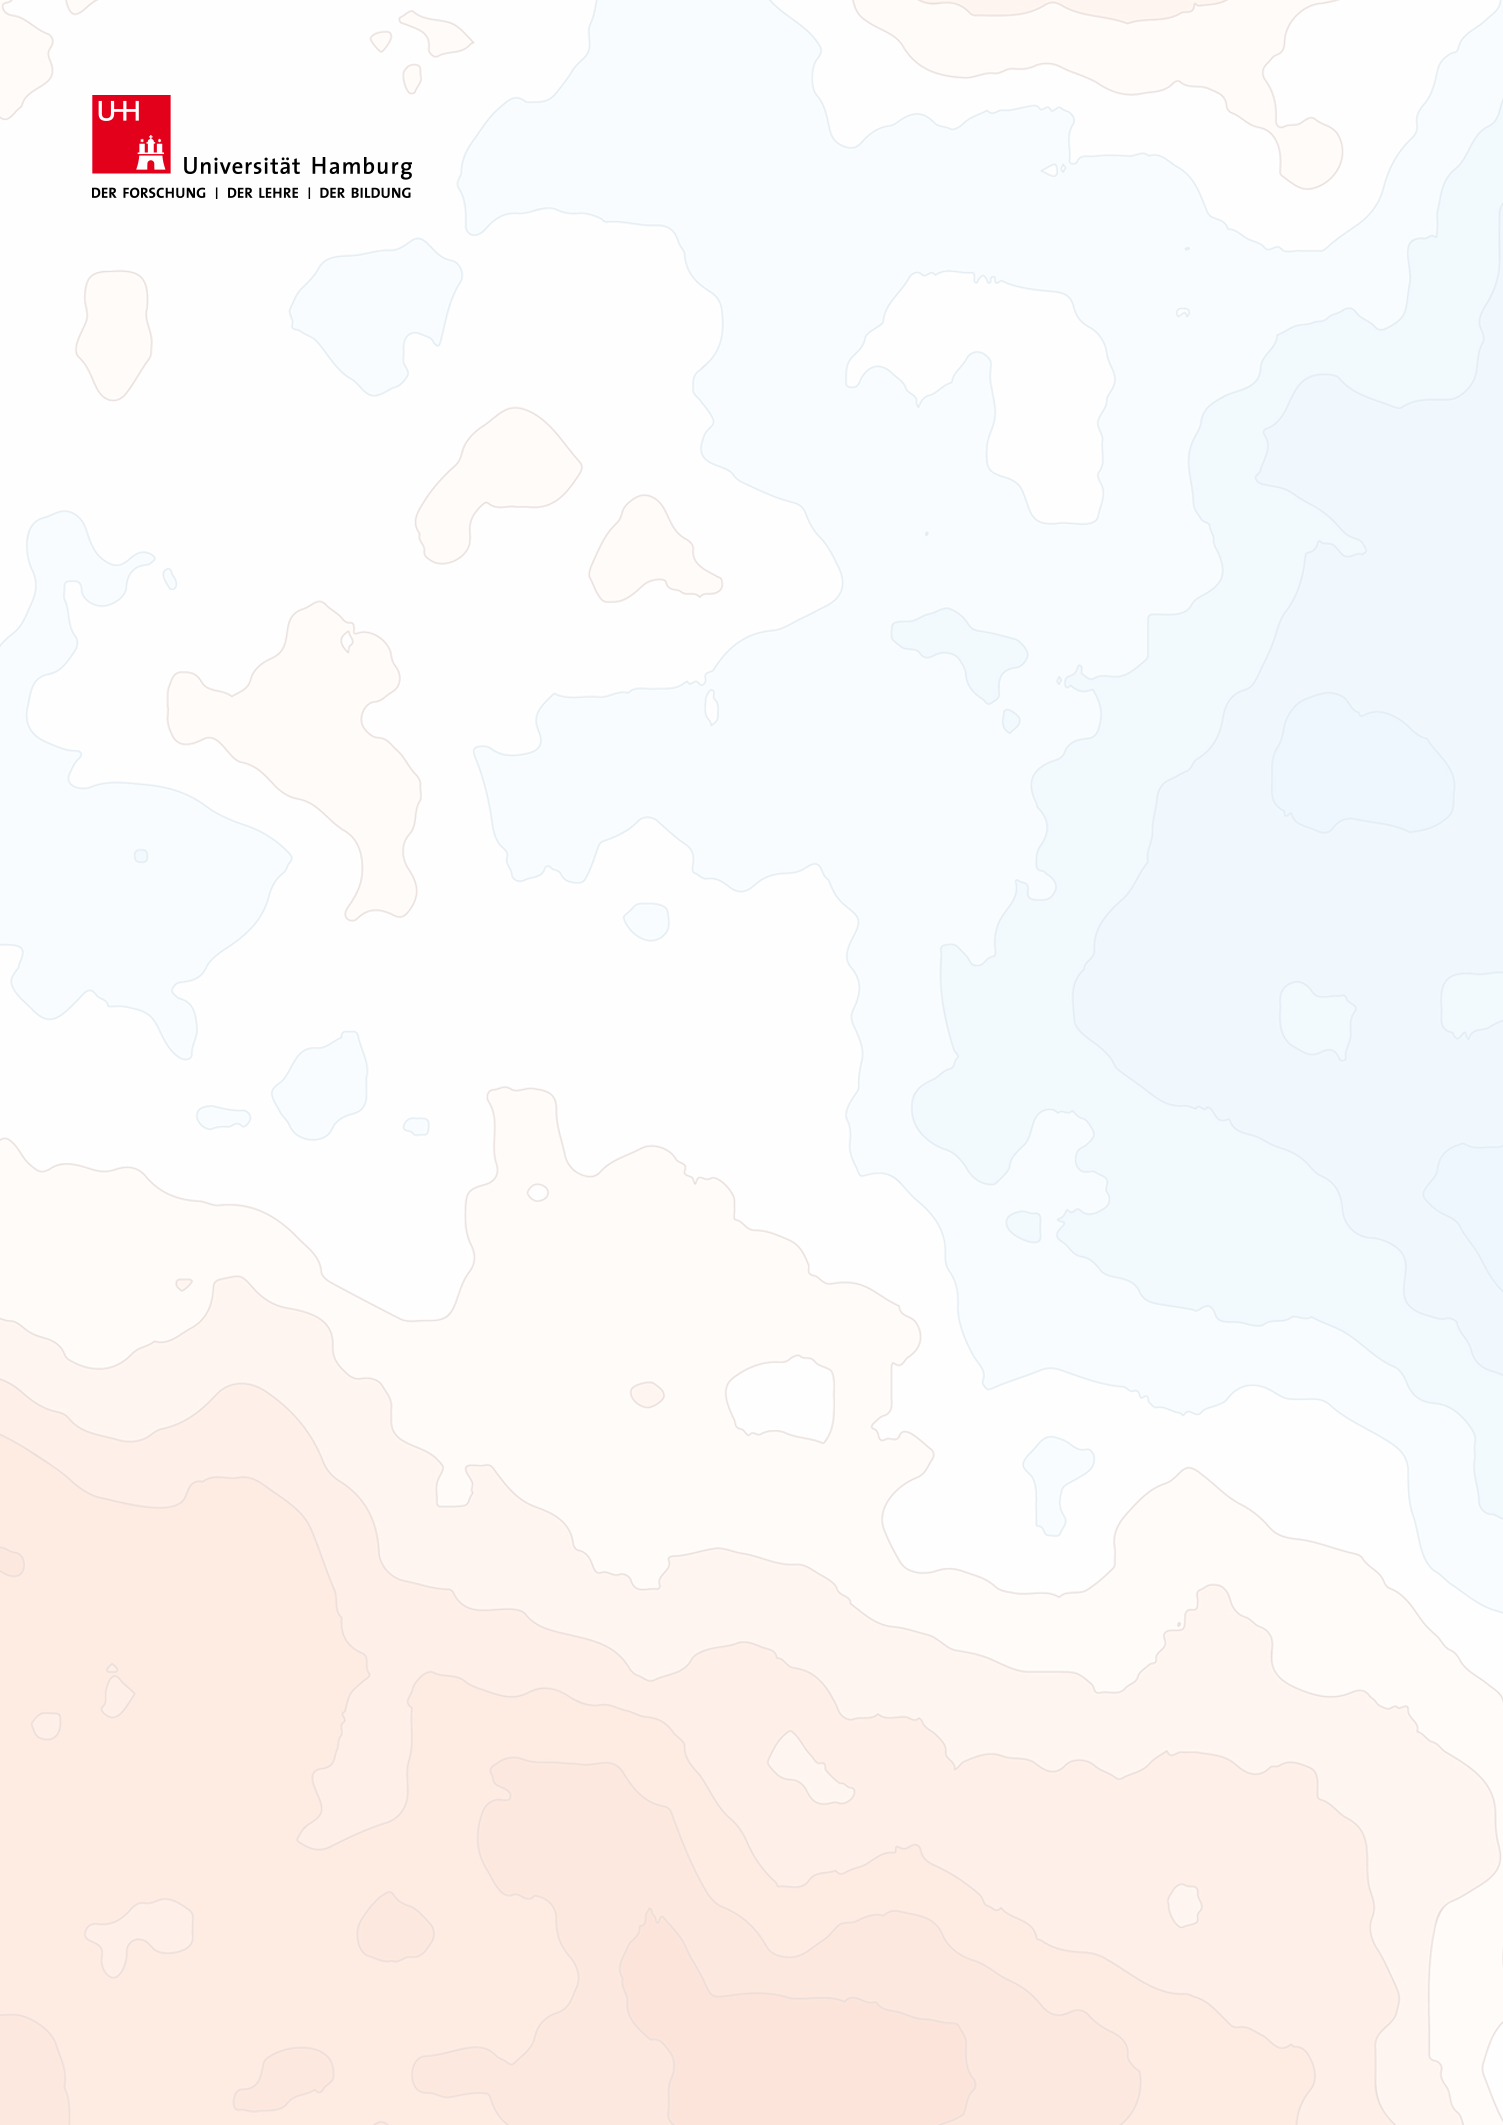
\includegraphics[width=\paperwidth,height=\paperheight,%
keepaspectratio]{resources/images/deckblatt.png}%
\vfill
}}}

\makeatletter
\newcommand*{\germanTitle}[1]{\gdef\@germanTitle{#1}}
\newcommand*{\englishTitle}[1]{\gdef\@englishTitle{#1}}
\newcommand*{\gradeType}[1]{\gdef\@gradeType{#1}}
\newcommand*{\firstExaminer}[1]{\gdef\@firstExaminer{#1}}
\newcommand*{\secondExaminer}[1]{\gdef\@secondExaminer{#1}}
\newcommand*{\matrikelnr}[1]{\gdef\@matrikelnr{#1}}
\newcommand*{\authorBirthplace}[1]{\gdef\@authorBirthplace{#1}}
\newcommand*{\submitDate}[1]{\gdef\@submitDate{#1}}
\newcommand*{\discipline}[1]{\gdef\@discipline{#1}}
\newcommand*{\courseOfStudies}[1]{\gdef\@courseOfStudies{#1}}
\newcommand*{\authorLastname}[1]{\gdef\@authorLastname{#1}}
\newcommand*{\authorFirstname}[1]{\gdef\@authorFirstname{#1}}

\renewcommand*{\maketitle}{
	\begin{titlepage}
		\newgeometry{left=3.8cm,right=2.5cm,top=4.6cm,bottom=2.5cm}
			\begingroup
				\fontsize{32pt}{32pt}\selectfont
				{\bfseries Bachelor Thesis}
			\endgroup

			\vskip 1.44cm

			\begingroup
			\fontsize{8pt}{6pt}\selectfont
			Title of the Thesis // Titel der Arbeit
			\endgroup

			\vskip -0.02cm

			\begingroup
			\fontsize{14pt}{14pt}\selectfont
			{\bfseries \@englishTitle\par}
			\vspace{0.3cm} % Add vertical space between German and English title
			{\@germanTitle\par}
			\endgroup
			\vskip -0.1cm

			\noindent\rule{15cm}{0.4pt}
			
			\vskip 0.05cm

			\begingroup
			\fontsize{8pt}{6pt}\selectfont
			Academic Degree // Akademischer Grad
			\endgroup

			\vskip -0.15cm

			\begingroup
			\fontsize{12pt}{14pt}\selectfont
				{\@gradeType}
			\endgroup
			\vskip -0.15cm

			\noindent\rule{15cm}{0.4pt}
			
			\vskip 0.05cm

			\begingroup
			\fontsize{8pt}{6pt}\selectfont
			Author's Name, Place of Birth // Name der Autorin/des Autors, Geburtsort
			\endgroup

			\vskip -0.15cm

			\begingroup
			\fontsize{12pt}{14pt}\selectfont
				{\@authorFirstname} {\@authorLastname}, {\@authorBirthplace}
			\endgroup
			\vskip -0.15cm

			\noindent\rule{15cm}{0.4pt}
			
			\vskip 0.05cm

			\begingroup
			\fontsize{8pt}{6pt}\selectfont
			Field of Study // Studiengang
			\endgroup

			\vskip -0.15cm

			\begingroup
			\fontsize{12pt}{14pt}\selectfont
				{\@courseOfStudies}
			\endgroup
			\vskip -0.15cm

			\noindent\rule{15cm}{0.4pt}
			
			\vskip 0.05cm

			\begingroup
			\fontsize{8pt}{6pt}\selectfont
			Department // Fachbereich
			\endgroup

			\vskip -0.15cm

			\begingroup
			\fontsize{12pt}{14pt}\selectfont
				{\@discipline}
			\endgroup
			\vskip -0.15cm

			\noindent\rule{15cm}{0.4pt}
			
			\vskip 0.05cm

			\begingroup
			\fontsize{8pt}{6pt}\selectfont
			First Examiner // Erstprüferin/Erstprüfer
			\endgroup

			\vskip -0.15cm

			\begingroup
			\fontsize{12pt}{14pt}\selectfont
				{\@firstExaminer}
			\endgroup
			\vskip -0.15cm

			\noindent\rule{15cm}{0.4pt}
			
			\vskip 0.05cm

			\begingroup
			\fontsize{8pt}{6pt}\selectfont
			Second Examiner // Zweitprüferin/Zweitprüfer
			\endgroup

			\vskip -0.15cm

			\begingroup
			\fontsize{12pt}{14pt}\selectfont
				{\@secondExaminer}
			\endgroup
			\vskip -0.15cm

			\noindent\rule{15cm}{0.4pt}
			
			\vskip 0.05cm

			\begingroup
			\fontsize{8pt}{6pt}\selectfont
			Matriculation Number // Matrikelnummer
			\endgroup

			\vskip -0.15cm

			\begingroup
			\fontsize{12pt}{14pt}\selectfont
				{\@matrikelnr}
			\endgroup
			\vskip -0.15cm

			\noindent\rule{15cm}{0.4pt}

			\vskip 0.05cm

			\begingroup
			\fontsize{8pt}{6pt}\selectfont
			Date of Submission // Abgabedatum
			\endgroup

			\vskip -0.15cm

			\begingroup
			\fontsize{12pt}{14pt}\selectfont
				{\@submitDate}
			\endgroup
			\vskip -0.15cm

			\noindent\rule{15cm}{0.4pt}
		\restoregeometry
	\end{titlepage}
}
\makeatother

% Variablen für das Deckblatt
\gradeType{Bachelor of Science (B.Sc.)}
\germanTitle{Wissenschaftliche Softwareentwicklung eines Convolutional Neuronal Networks für die Rekonstruktion fehlender Daten einer Wettermessstation unter Verwendung von Numerischen Modelldaten}
\englishTitle{Scientific software development of a Convolutional Neural Network for the reconstruction of missing data from a weather measurement station using numerical model data.}
\authorFirstname{Timo}
\authorLastname{Wacke}
\authorBirthplace{Hamburg}
\discipline{Computer Science // Informatik}
\courseOfStudies{Computing in Science (Physics Specialization)}
\matrikelnr{7434883}
\submitDate{10.06.2024}
\firstExaminer{Prof. Dr. Thomas Ludwig}
\secondExaminer{Dr. Christopher Kadow}


\makeatletter

\newcommand*{\place}[1]{\gdef\@place{#1}}

\newcommand*{\makeeidesstatt}{
	\begin{titlepage}
		\newgeometry{left=3.8cm,right=2.5cm,top=8cm,bottom=2.5cm}
			\begingroup
			\fontsize{18pt}{20pt}\selectfont
			{\bfseries Eidesstattliche Versicherung}
			\endgroup

			\vskip 0.8cm

			\begingroup
			\fontsize{12pt}{14pt}\selectfont
				{\@authorLastname} {\@authorFirstname}
			\endgroup

			\vskip -0.5cm

			\noindent\rule{15cm}{0.4pt}

			\vskip -0.4cm

			\begingroup
			\fontsize{8pt}{6pt}\selectfont
			Last Name, First Name // Name, Vorname
			\endgroup

			\vskip 0.6cm
			\begingroup
			\fontsize{10.5pt}{11.5pt}\selectfont
   
			„Hiermit versichere ich an Eides statt, dass ich die vorliegende Arbeit mit dem Titel
			\endgroup

			\begingroup
			\fontsize{16pt}{18pt}\selectfont
			{\bfseries \@germanTitle}
			\endgroup

			\begingroup
			\fontsize{10.5pt}{11.5pt}\selectfont
			im Bachelorstudiengang \@courseOfStudies selbstständig verfasst und keine anderen als die angegebenen Hilfsmittel – insbesondere keine im Quellenverzeichnis nicht benannten Internet-Quellen – benutzt habe. Alle Stellen, die wörtlich oder sinngemäß aus Veröffentlichungen entnommen wurden, sind als solche kenntlich gemacht. Ich versichere weiterhin, dass ich die Arbeit vorher nicht in einem anderen Prüfungsverfahren eingereicht habe.
			\endgroup

			\vskip 0.8cm

			{
			\fontsize{12pt}{14pt}\selectfont
			{\@place}, den {\today}
			}

			\vskip -0.5cm

			\noindent\rule{15cm}{0.4pt}

			\vskip -0.3cm

			\begingroup
			\fontsize{8pt}{6pt}\selectfont
			Place, Date, Signature // Ort, Datum, Unterschrift
			\endgroup


		\restoregeometry
	\end{titlepage}}
\makeatother

\place{Hamburg}


\lstset{literate=%
  {Ö}{{\"O}}1
  {Ä}{{\"A}}1
  {Ü}{{\"U}}1
  {ß}{{\ss}}1
  {ü}{{\"u}}1
  {ä}{{\"a}}1
  {ö}{{\"o}}1
}

% Javascript als Sprache für die lstings
\lstdefinelanguage{JavaScript}{
  keywords={typeof, new, true, false, catch, function, return, null, catch, switch, var, if, in, while, do, else, case, break, that, globals, let, const},
  keywordstyle=\color{blue}\bfseries,
  ndkeywords={class, export, boolean, throw, implements, import, this},
  ndkeywordstyle=\color{darkgray}\bfseries,
  identifierstyle=\color{black},
  sensitive=false,
  comment=[l]{//},
  morecomment=[s]{/*}{*/},
  commentstyle=\color{gray}\ttfamily,
  stringstyle=\color{red}\ttfamily,
  morestring=[b]',
  morestring=[b]"
}
\lstset{
    language=JavaScript,
    numbers=none,
    frame=leftline,
    tabsize=2,
    rulesepcolor=\color{gray},
    rulecolor=\color{black},
    captionpos=b,
    breaklines=true,
    breakatwhitespace=false,
}

\lstdefinelanguage{Python}{
    keywords={self, def, class, import, from, if, else, elif, for, while, return, True, False, None},
    keywordstyle=\color{blue}\bfseries,
    ndkeywords={},
    ndkeywordstyle=\color{darkgray}\bfseries,
    identifierstyle=\color{black},
    sensitive=true,
    comment=[l]{\#},
    morecomment=[s]{"""}{"""},
    commentstyle=\color{gray}\ttfamily,
    stringstyle=\color{orange}\ttfamily,
    morestring=[b]',
    morestring=[b]"
}

\lstset{
    language=Python,
    numbers=none,
    frame=leftline,
    tabsize=2,
    rulesepcolor=\color{gray},
    rulecolor=\color{black},
    captionpos=b,
    breaklines=true,
    breakatwhitespace=false,
}

\newcommand{\subsubsubsection}[1]{\paragraph{#1}\mbox{}\\}
\setcounter{secnumdepth}{4}
\setcounter{tocdepth}{4}
\begin{document}

% Entfernen der Seitenzahlen und BackroundPic als Hintergrund nutzen
\pagenumbering{gobble}
\AddToShipoutPicture{\BackgroundPic}

% Titelblatt erzeugen
\maketitle
\newpage

% Eidesstattliche Erklärung erzeugen
\makeeidesstatt
\thispagestyle{empty}

% Abstract und Inhaltsverzeichnisse einfügen (Numerierung römisch ab Inhaltsverzeichnis)
\section*{Abstract}
\label{sec:abstract}
\section*{Zusammenfassung}

\ClearShipoutPicture
\thispagestyle{empty}
\newpage
\pagenumbering{Roman}
\tableofcontents
\newpage
\listoffigures
\newpage

% Kapitel einfügen
\pagenumbering{arabic}
\section{Introduction}
\label{sec:introduction}

% Weather stations are sparse in some regions

Weather station density varies greatly across the globe, depending on population density, economic development, and access to nearby infrastructure \cite{ortizbobea2021}. While any weather station can experience downtime, the reliability of weather stations in regions with low station density is often low as well \cite{Mistry2022GlobalWeatherStations}. So not only is downtime in regions where data is limited more likely but also more impactful because there are fewer neighboring stations to help compensate for the missing data.

A denser, more reliable network would benefit weather forecasting, helping to evacuate populations timely before natural disasters \cite{muita2021} and from a global perspective aiding climate research. For example in East Africa, the weather station density is very low, but the region would be of great interest to the El Niño Southern Oscillation (ENSO) research. The irregular fluctuation between El Niño and La Niña phases affects the climate from the tropics to even higher-latitude regions through teleconnections \cite{marchant2007, muita2021}.  An innovative approach to increase the density of weather stations could be to use low-cost weather stations that could be 3D-printed and assembled by the local population \cite{muita2021}. Either way, low-cost weather stations have reliability issues and are prone to downtime, as outlined in section \ref{sec:3d_printed_stations}.

% Let's connect aerial data with local measurements

In light of the challenges posed by sparse weather station coverage, novel methodologies are required to address the reconstruction of missing weather data. One promising approach is to apply machine learning techniques, which offer a departure from traditional numerical reconstruction methods such as kriging, that rely on neighboring station data and are often computationally intensive \cite{chung2019kriging}. The application of machine learning, in this case, would be to relate coarse-resolution numerical reanalysis data, which in itself can not accurately describe the local characteristics, to the local patterns at the weather station. This would allow for independent operation, without relying on neighboring stations or additional data sources. It can directly utilize the global reanalysis data as input, outperforming numerical methods in terms of computational resource requirements by orders of magnitude \cite{kurth2023MLperformance,bi2023MLperformance,lam2023MLperformance} as the application of the trained machine-learning model. By leveraging available local data, these techniques, such as Convolutional Neural Networks (CNNs), can be trained to estimate weather conditions at a designated time by assimilating global numerical weather model data. Despite the inherent blurriness of aerial data provided in grid cells, these models are anticipated to discern and adapt to local weather patterns such that they become capable of transferring knowledge from the meta situation to the local situation. This paper aims to achieve reconstruction using that approach which will be further explained in \autoref{sec: design}.

% ERA5 0.25 hourly everywhere

The reanalysis of choice in this endeavor is the ECMWF Reanalysis v5 (ERA5), which covers the globe in grid cells of 0.25° x 0.25°. The data is available in hourly timesteps from 1940 to the present and contains a wide range of variables, such as temperature, precipitation, wind speed, and many more. \cite{era5}

% Let's go with the temperature

To prove the concept it's likely easiest to start with temperature data, meaning the 2m temperature variable from the ERA5 reanalysis will be used as input to the neural net.
%, one hour at a time, and the expected output will be the temperature at the weather station, during the same hour.
\section{3D printed Weather Stations}
\label{sec:3d_printed_stations}

3D-Printed automated weather stations (3D-PAWS) are low-cost, compact automatic weather stations designed to expand meteorological observation networks, especially in data-sparse regions. They are equipped with sensors to measure various meteorological parameters like temperature, humidity, wind speed/direction, rainfall, and surface pressure. The station components (housing, sensor mounts, etc.) are 3D printed using durable plastic materials, making them lightweight and easy to deploy \cite{mwangi2017paws}.

% Comparison with Traditional Stations

The study compared data from a 3D-PAWS unit co-located with a manual synoptic weather station and a TAHMO automatic station in Kenya. Strong correlations were found between 3D-PAWS and the manual station for maximum temperature (r=0.59) and surface pressure (r=0.65). However, 3D-PAWS showed a high positive bias (~10°C) for minimum temperature readings, likely due to battery issues during non-daylight hours. Correlations were weaker for wind speed, wind direction, and rainfall between 3D-PAWS and the other stations \cite{mwangi2017paws}.

% Advantages and Challenges

3D-PAWS offer a cost-effective way to densify weather observation networks, especially in regions with limited resources. Their compact size and 3D-printed construction make them easy to transport and install in remote locations. Continuous monitoring and maintenance are crucial to ensure consistent data quality, as issues like battery failure can introduce biases. Further calibration and validation studies are needed to establish the reliability of 3D-PAWS data for various meteorological applications \cite{mwangi2017paws}.

In summary, 3D-PAWS represent an innovative approach to expanding weather monitoring capabilities using additive manufacturing technology. While showing promise, ongoing efforts are required to improve their data quality and reliability for widespread adoption \cite{mwangi2017paws}.

\section{Conceptual Framework}
\label{sec:design}

\subsection{Concept}

\begin{figure}
    \centering
    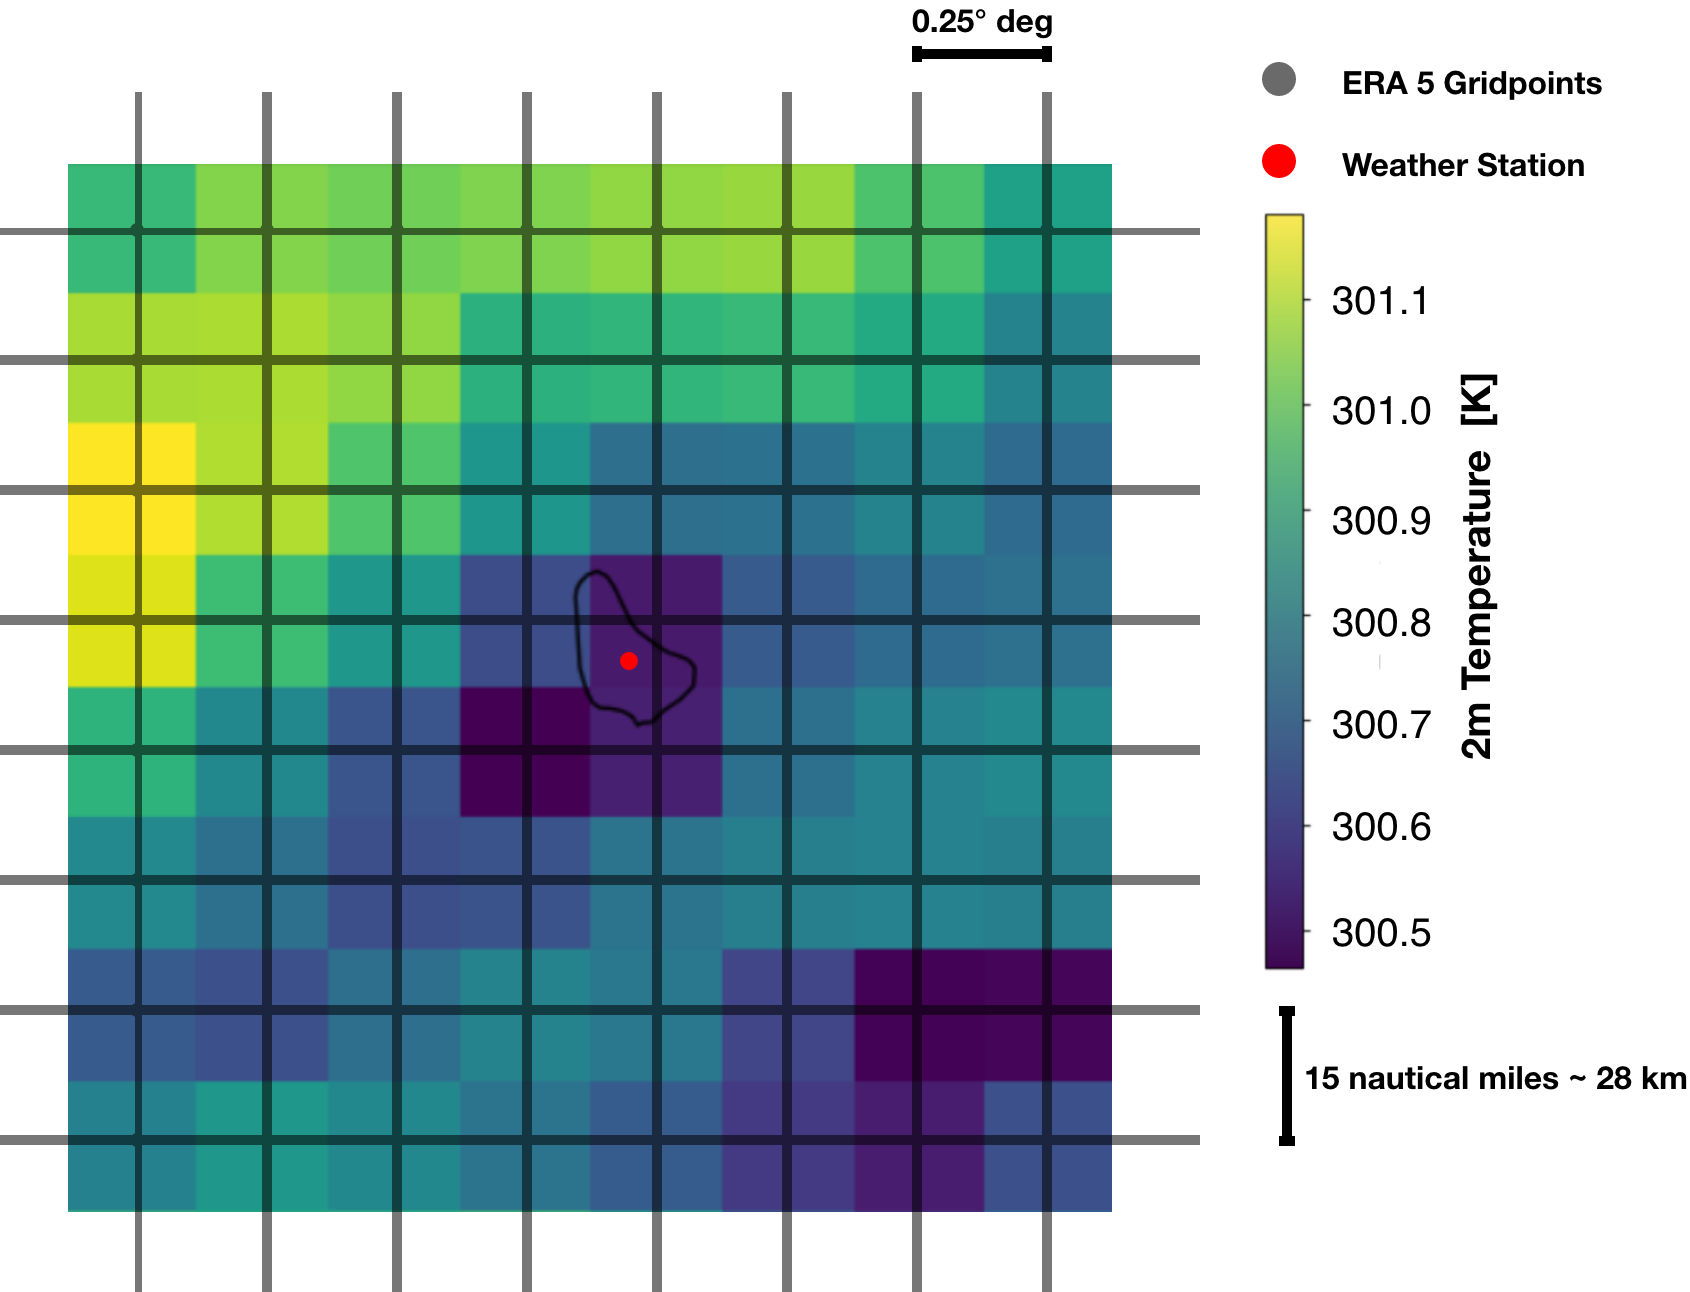
\includegraphics[width=\textwidth]{resources/images/ERA5_tas_around_barbados.png}
    \caption{8x8 grid-points of ERA5 with 2m temperature 
    for 2020-06-23 19:00 UTC  in the area of a weather station on Barbados}    
    \label{fig:barbados}
\end{figure}

\begin{figure}
    \centering
    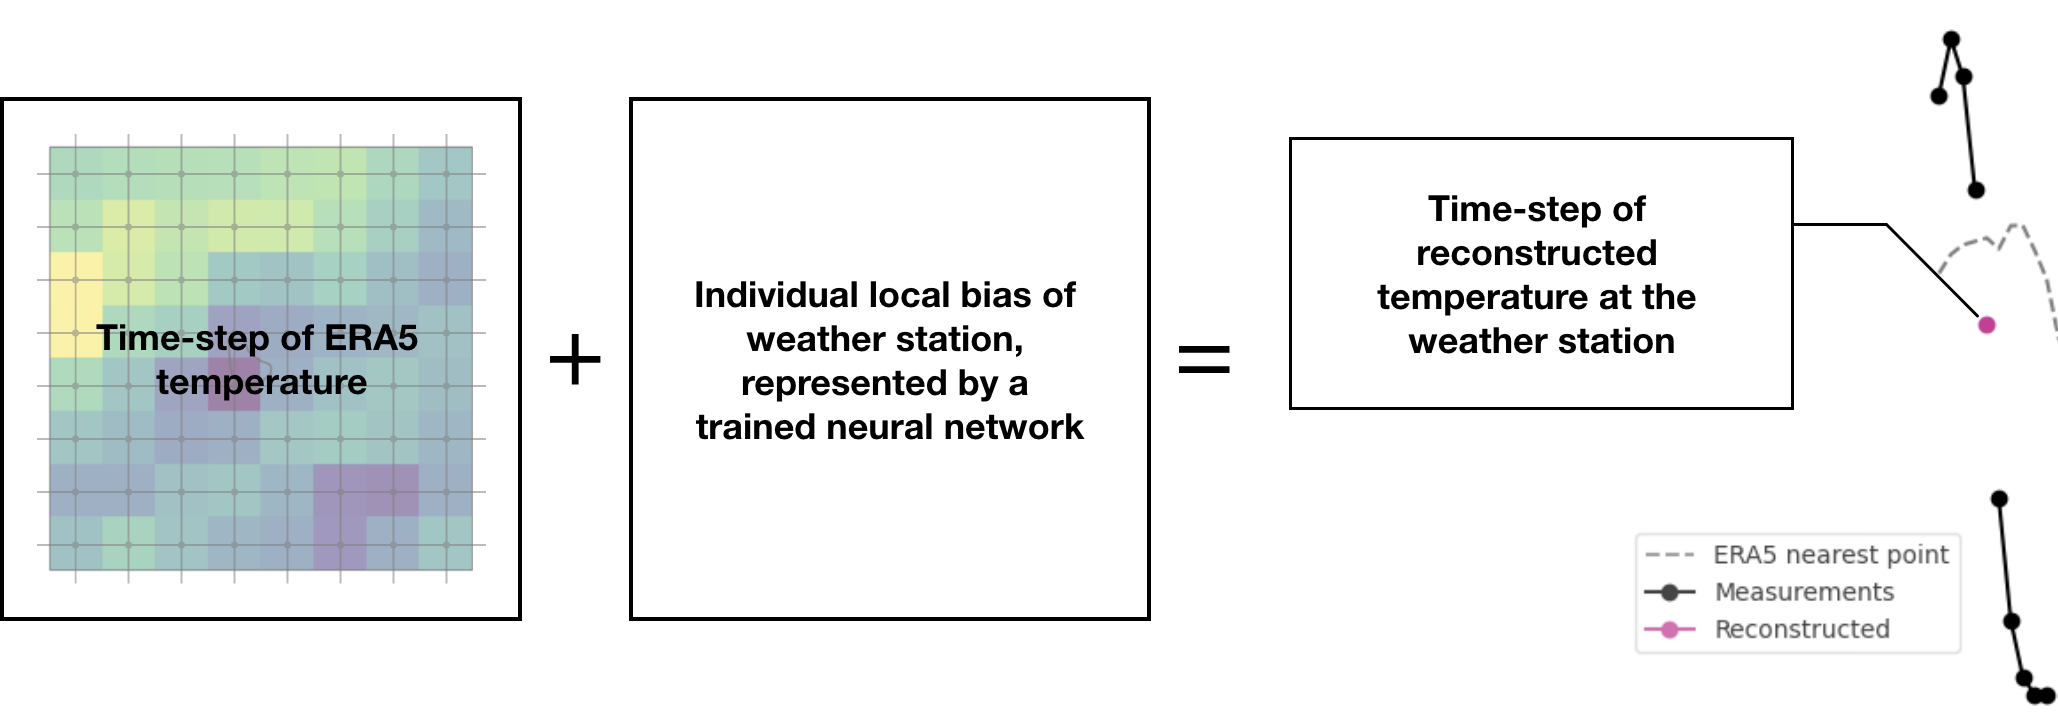
\includegraphics[width=450pt]{resources/images/digitaltwin_schema.png}
    \caption{Conceptual Framework of the proposed method}    
    \label{fig:concept}
\end{figure}

The conceptual framework of the proposed method is illustrated in \autoref{fig:concept}. Applying the local bias of the weather station against ERA5 on top of ERA5 would reconstruct the temperature data at the station. The idea is that a Convolutional Neural Network would learn the complex behaviour of the bias depending on the arial situation, if you train it with enough available measurments. Once the CNN is trained as a model that represents the local bias of the weather station vs the ERA5 data, applying it to the ERA5 data allows for the reconstruction of missing temperature values at the weather station just by providing the data of the ERA5 temperature in the regional cutout at that timestamp used in training as an input. To illustrate what such a bias could be: In the case of Barbados for example the grid cells of the ERA5 data all lay primarly in the ocean, meaning the diurnal cycle has a much lower amplitude than at the weather station that is placed on land, the neural network would need to learn how to detect based on the 64 grid points in which phase of the diurnal cycle the weather station is and then adjust the temperature values accordingly. Besides this obvious difference between ERA5 and the measurmenets at Barbados there are most likely many more local effects to master.

Since the ERA5 data is available everywhere and for any timestep, for any hour without measurements at the weather station that the model is trained for could be reconstructed. To train the model, a supvervised learning approach would be used, meaning that the input will be ERA5 data at times where measurements are available and the expected output should be the measurements at the weather station. The model would be trained to minimize the difference between the expected output and the model's prediction through backpropagation. To allow for flexibility in application and simplicity in training, the training has to be done hour by hour, meaning the model is passed during training one timestep at a time and the weights are updated between iterations. When reconstructing missed data, hence the model is applied to the ERA5 data hour by hour as well and the result is a series of hourly predictions that are not connected in time.

% In \autoref{fig:barbados} ERA5 grid points around a weather station on Barbados are shown along with their corresponding temperature two meters above the surface. The graph is for the hour 19:00 UTC on the 23rd of June 2020. Along the latitude and longitude lines 8 grid points are selected in each dimension, such that the weather station is centered, meaning it lays between the 4th and 5th grid point in each dimension. The available longitudes and latitudes in the ERA5 model are spaced by 0.25° along the latitude and longitude from each other, which means an almost fixed distance along the latitude while the width along the longitude varies depending on how close to the poles/equator the grid points are, obviously going close to zero neat the poles. In the case of Barbados at a latitude of 13 deg the distance between 2 gridpoints along the longitude is still about 27 km.

\subsection{Data Acquisition and Preprocessing}
\label{subsec:data_preprocessing}
Upon obtaining a dataset from a weather station, it is determined where temperature data is missing. While the weather station dataset is minute-based, data could be missing only for a few minutes within an hour instead of the full hour. This would raise the question of how many missing values are acceptable to not mark the hour as missing. Sure is, that if all temperature values are missing during an hour, the hour is marked as missing.
The ERA5 data then needs to be cropped to the neighboring 8x8 grid cells, while centering the cutout as close to the weather station as possible. The available longitudes and latitudes in the ERA5 model are spaced by 0.25° along the latitude and longitude from each other, when 8x8 grid cells are selected it needs to be assured that the grid points are such selected that the coordinates of the weather station are between the 4th and 5th grid point in each dimension. 
After cropping the ERA5 dataset geographically, the data needs to be cut and divided along the time axis to match the weather station data, leading to two datasets: one with all the hours marked as missing and one with all the hours marked as present. Until the model is trained, only the dataset with all the hours marked as present will be used. 

As a result we have a dataset pair of weather station measurements and ERA5 data, that are coherant in time and space.

To determine after the training if and to which extent the model learned to reconstruct the missing data, the dataset pair is split again alogn the timeaxis into a pair of station with ERA5 data for training and oair of station with ERA5 data for validation. Thus we can later let the model reconstruct values that have actually been measured but haven't been included in the training so we then can validate how successful the reconstruction is. With the datasets prepared, the next phase involves configuring and training the Convolutional Neural Network (CNN) for the temperature reconstruction task. The CNN architecture is tailored to accept input in the form of 8x8 grid cells centered around the weather station's location. Employing a supervised learning approach, the CNN is trained using pairs of hourly temperature data from the weather station and corresponding grid cell data from ERA5. The training process iteratively feeds batches of data into the CNN, fine-tuning its parameters to minimize prediction errors and optimize accuracy in reconstructing missing temperature values.


\subsection{Model Evaluation}
Following the training phase, the CNN's performance is evaluated using the validation set. The model's capacity to accurately reconstruct missing temperature data at the weather station is scrutinized against ground truth values. This evaluation step serves to gauge the CNN's proficiency in capturing intricate weather patterns and producing precise temperature estimations. For that, the root mean squared error (RMSE) and the correlation coefficient are calculated. The RMSE is a measure of the differences between predicted and observed values, while the correlation coefficient quantifies the strength and direction of the linear relationship between the two datasets. An obvious choice as timerange for the evaluation would be to cut out one complete year so that the model can be evaluated over the full range of seasons and weather conditions. 

\subsection{Application to New Data}
Upon successful training and validation, the model is trained again with the measurements that have been exluded before in the benefit of validation. After training on the full data the CNN can be used to fill gaps. Fundamentally any list of timesteps that the model should applied for can be requested and then the ERA5 data for the respective timesteps is optained, cropped in the same way to the geographical region as before and then the model is applied to the data. The result is a list of temperature values that are not connected in time, but are the model's prediction for the temperature at the weather station at the respective time. Since in \ref{subsec:data_preprocessing} we split the ERA5 dataset already into two datasets, one with all hours marked as missing and one with all hours marked as present, the model can be applied to the dataset with all hours marked as missing and then directly infilled into the original measurements dataset.
\section{Theoretical Background}
\label{sec:theory}

\subsection{Convolutional Neural Networks}
\label{subsec:cnn}

Convolutional neural networks (CNNs) have excelled at extracting patterns and features from spatial data such as satellite imagery, radar data, and climate model outputs. This capability has enabled researchers to better understand and predict complex atmospheric and oceanic phenomena. For instance, CNNs have been employed to detect and localize extreme weather events from satellite data, enhancing early warning systems and disaster response efforts. Furthermore, CNNs have improved the ability to identify forced climate patterns and disentangle natural variability from human-induced climate change signals, advancing our understanding of climate dynamics and informing mitigation strategies.


CNNs are a type of deep learning architecture inspired by the visual cortex of animals. They are designed to efficiently capture spatial and temporal dependencies in data through the use of learnable filters and hierarchical feature representations. Through the use of convolutional layers instead of fully connected layers, the architecture is able to preserve the spatial structure of the input data, making it particularly well-suited for image and video data. This approach not only simplifies pattern detection but also implies a reduction in the number of parameters, which minimizes the necessary computational resources.

Application of CNNs in climate science has yielded several notable contributions, including the reconstruction of the El Nino event of 1877 by Kadow et al. despite extremely limited data availability. \cite{kadow2020}

In the context of this work an architecture introduced by (\cite{ronneberger2015}) is used, which consists of an encoder and a decoder part as seen in \autoref{fig:u_net}. Due to it's shape it is called U-Net. The encoder part consists of convolutional layers and pooling layers, while the decoder part consists of upscaling layers and in this case, skip connections as proposed by \cite{liu2018inpaining}.

\subsubsection*{Convolutional Layer}
\begin{figure}
    \centering
    \animategraphics[loop,autoplay,width=400pt]{1}{resources/images/convolution_gif/convolution_kernel-}{0}{15}
    \caption{How a convolution operation works. \cite{datahacker}}
    \label{fig:convolution_operation}
\end{figure}

The convolutional layer is the driver for feature mapping in a CNN. It applies a convolution operation shown in \autoref{fig:convolution_operation} to the input data. The operation is done element by element while sliding a filter (also called kernel) over the input data such that situations, where the filter overflows the input data ranges, are avoided or taken care of. On each step, the Frobenius Product between the kernel and the submatrix given by the current position and the kernel dimension is calculated and noted in the output matrix. The parameters in the kernel matrix are chosen in such a way that the Frobenius Product is maximized when the kernel is over a feature that the kernel is supposed to detect. In \autoref{fig:convolution_operation} the kernel for example is a vertical edge detector, meaning it will output a high amount (positive or negative) when the horizontal gradient in the input data submatrix has a high absolute value. This result is rather trivial, as a positive horizontal gradient as seen in the upper-left 3x3 submatrix of the example leads to a right column that when negatively weighted overweights the positive-weighted left column and thus the output for the upper-left 3x3 submatrix is negative. Conversely, a Fresenius product of the upper-right 3x3 submatrix with the kernel returns a positive value, hinting at a negative horizontal gradient in the input data. The result of such a convolution can be observed in \autoref{fig:edge_detection}.

In the context of weather data, the convolutional layer can be used to detect any weather patterns not just edges and the kernel itself can be learned by the network.

\begin{figure}
    \centering
    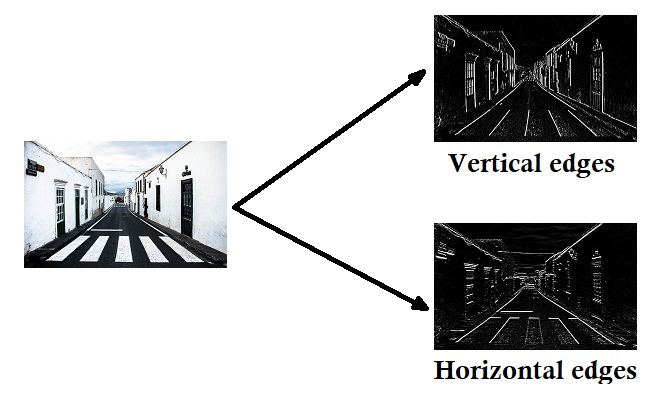
\includegraphics[width=250px]{resources/images/edge_detection.jpeg}
    \caption{Example of edge detection with a convolutional kernel. \cite{datahacker}}
    \label{fig:edge_detection}
\end{figure}

\subsubsection*{Activation Function}

To map the output of the convolutional layer to a meaningful space, and to avoid negative values, an activation function is applied. This introduces non-linearity into the network. The simplest activation function is the ReLU function, which returns the input if it is positive and zero otherwise. It is defined as $f(x) = max(0, x)$. The ReLu function is the activation function used in this work after each convolutional operation.

\subsubsection*{Pooling Layer}

The exact position of a low-level feature in the input data is not so important when it comes to detecting high-level features,
it is more important to recognize if a feature is present at all in certain spatial areas of the input data or not.
Thus scaling down the resolution of the matrix by combining every 2x2 submatrix into one value can be beneficial.
It is most commonly aggregated by taking the maximum value of the submatrix because it works for the mentioned purpose to detect if a feature is present in the area of the submatrix or not. While the convolution layer depending on how the convolution is processed near the borders of the input data reduces the dimensionality of the input data just slightly or not at all, the pooling reduces the dimensionality drastically. So after a 2x2 pooling operation, the output matrix is only a quarter of the size of the input matrix.

\begin{figure}
    \begin{subfigure}{1\textwidth}
        \centering
        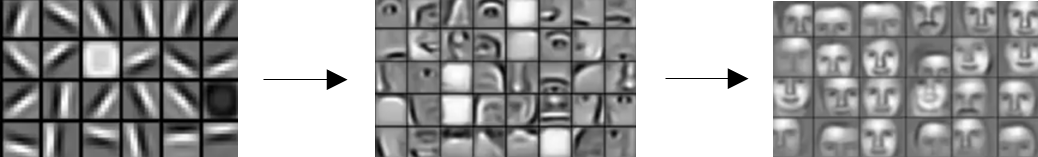
\includegraphics[width=0.9\textwidth]{resources/images/abstraction.png}
        \caption{Low-level features are combined into high-level features.}
        \label{fig:abstraction}
    \end{subfigure}
    \vspace{0.5cm}
    \begin{subfigure}{0.65\textwidth}
        \centering
        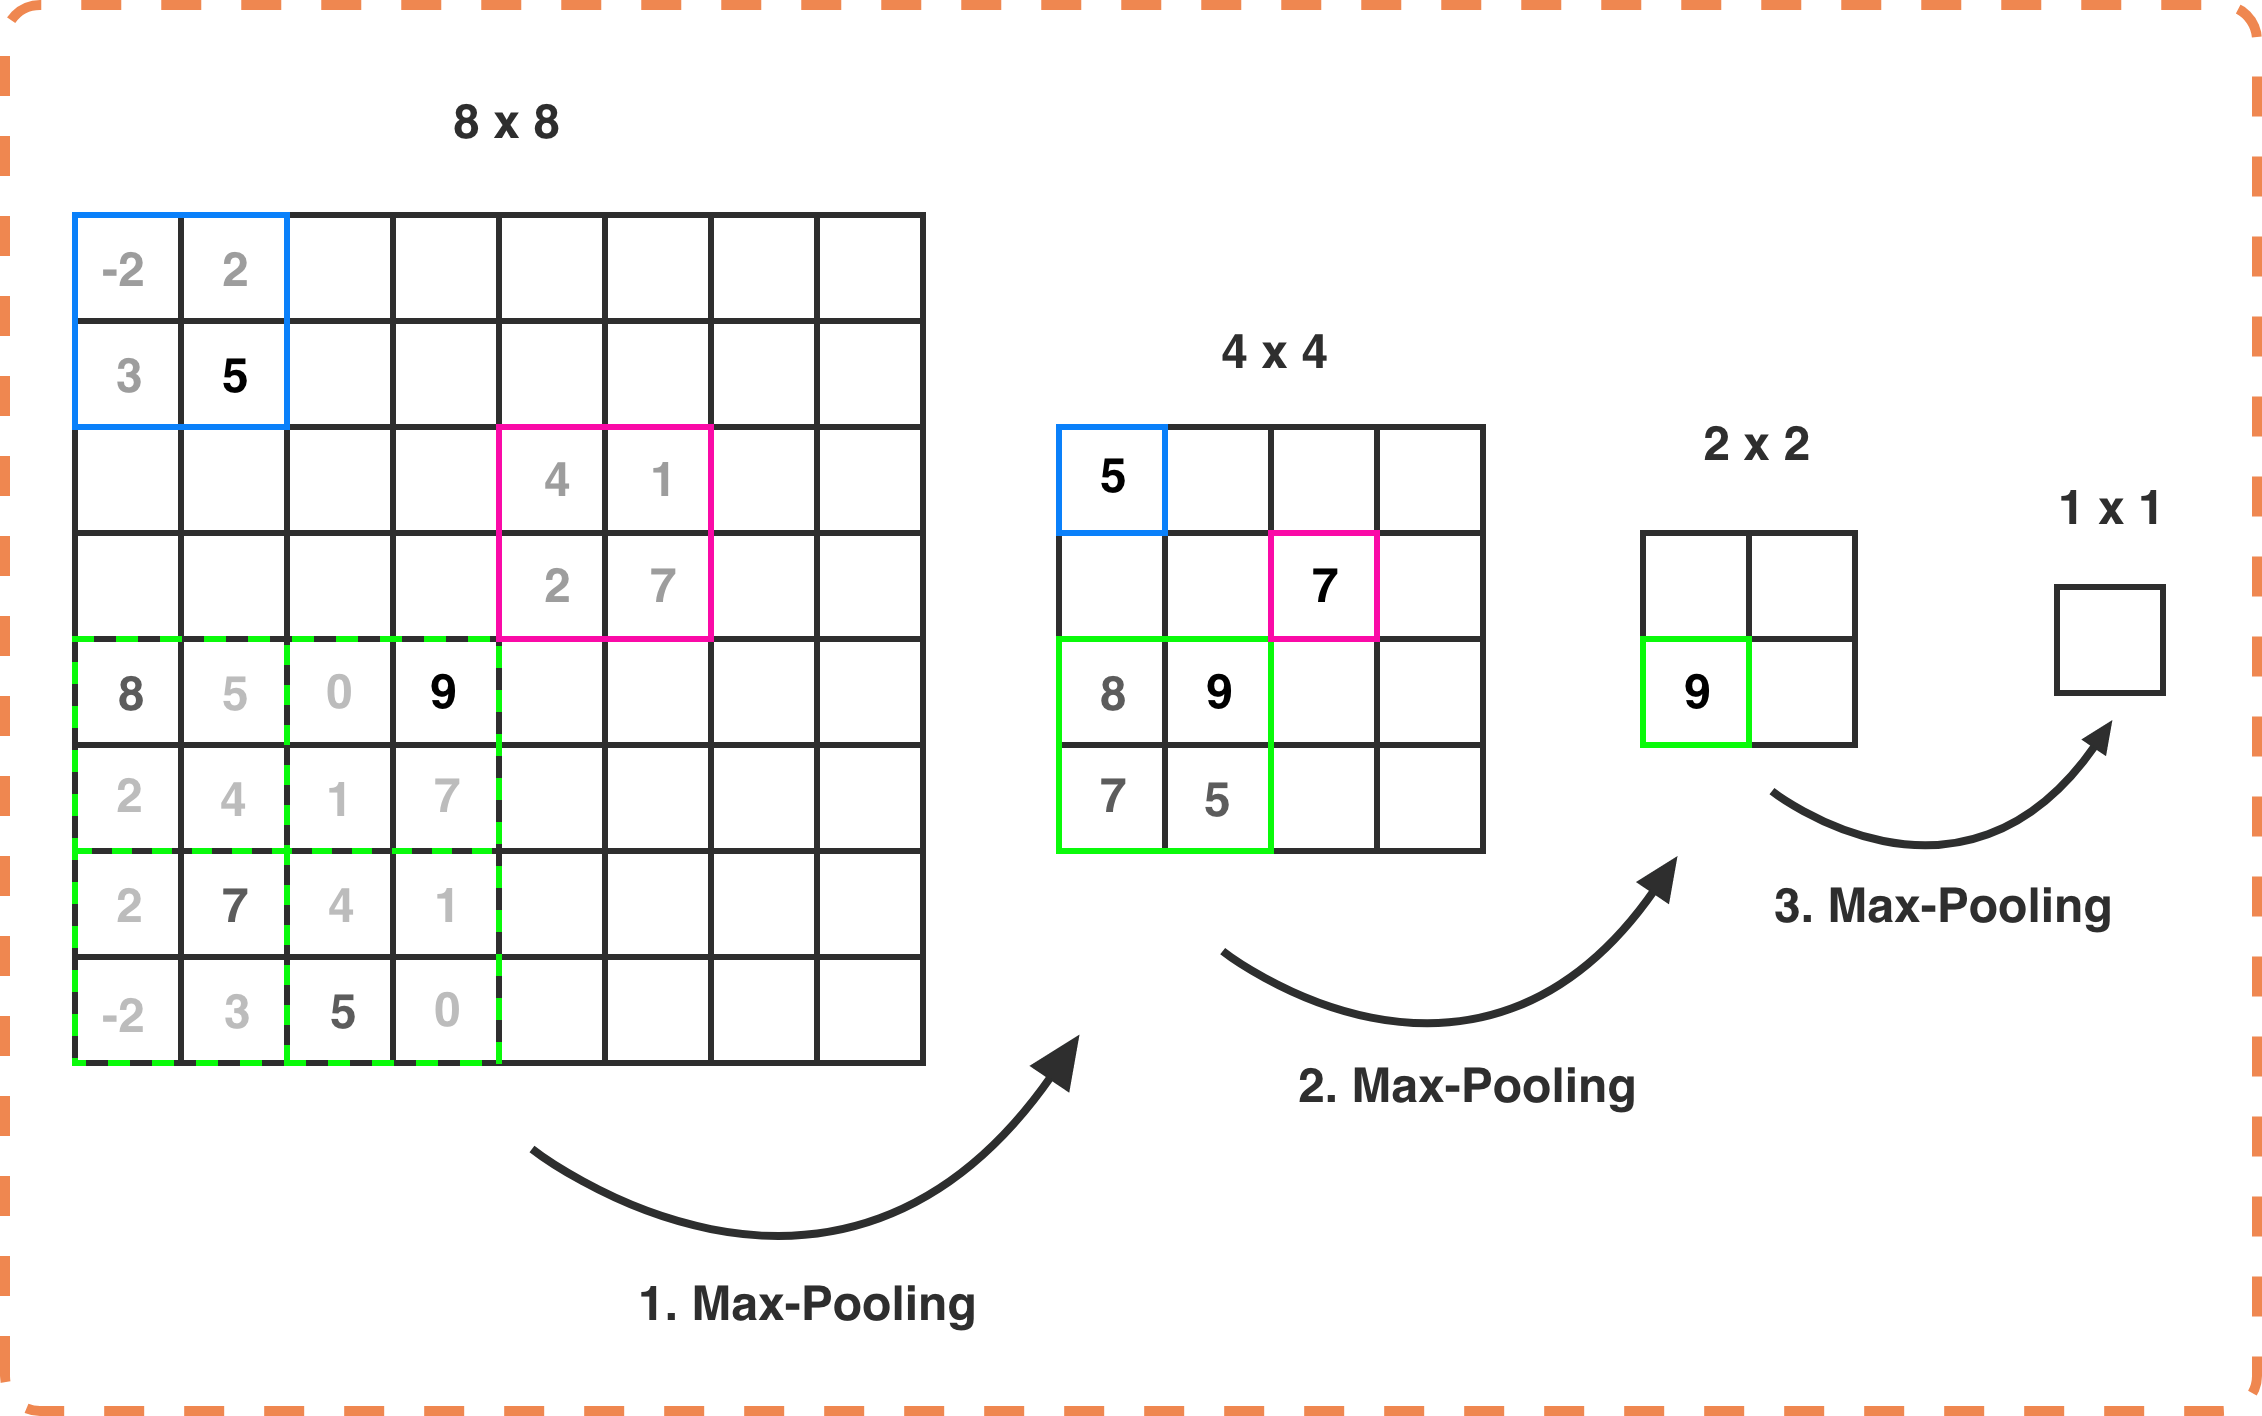
\includegraphics[width=\textwidth]{resources/images/max_pooling.png}
        \caption{Illustration of 3 max pooling operations}
        \label{fig:max_pooling}
    \end{subfigure}
    \begin{subfigure}{0.30\textwidth}
        \centering
        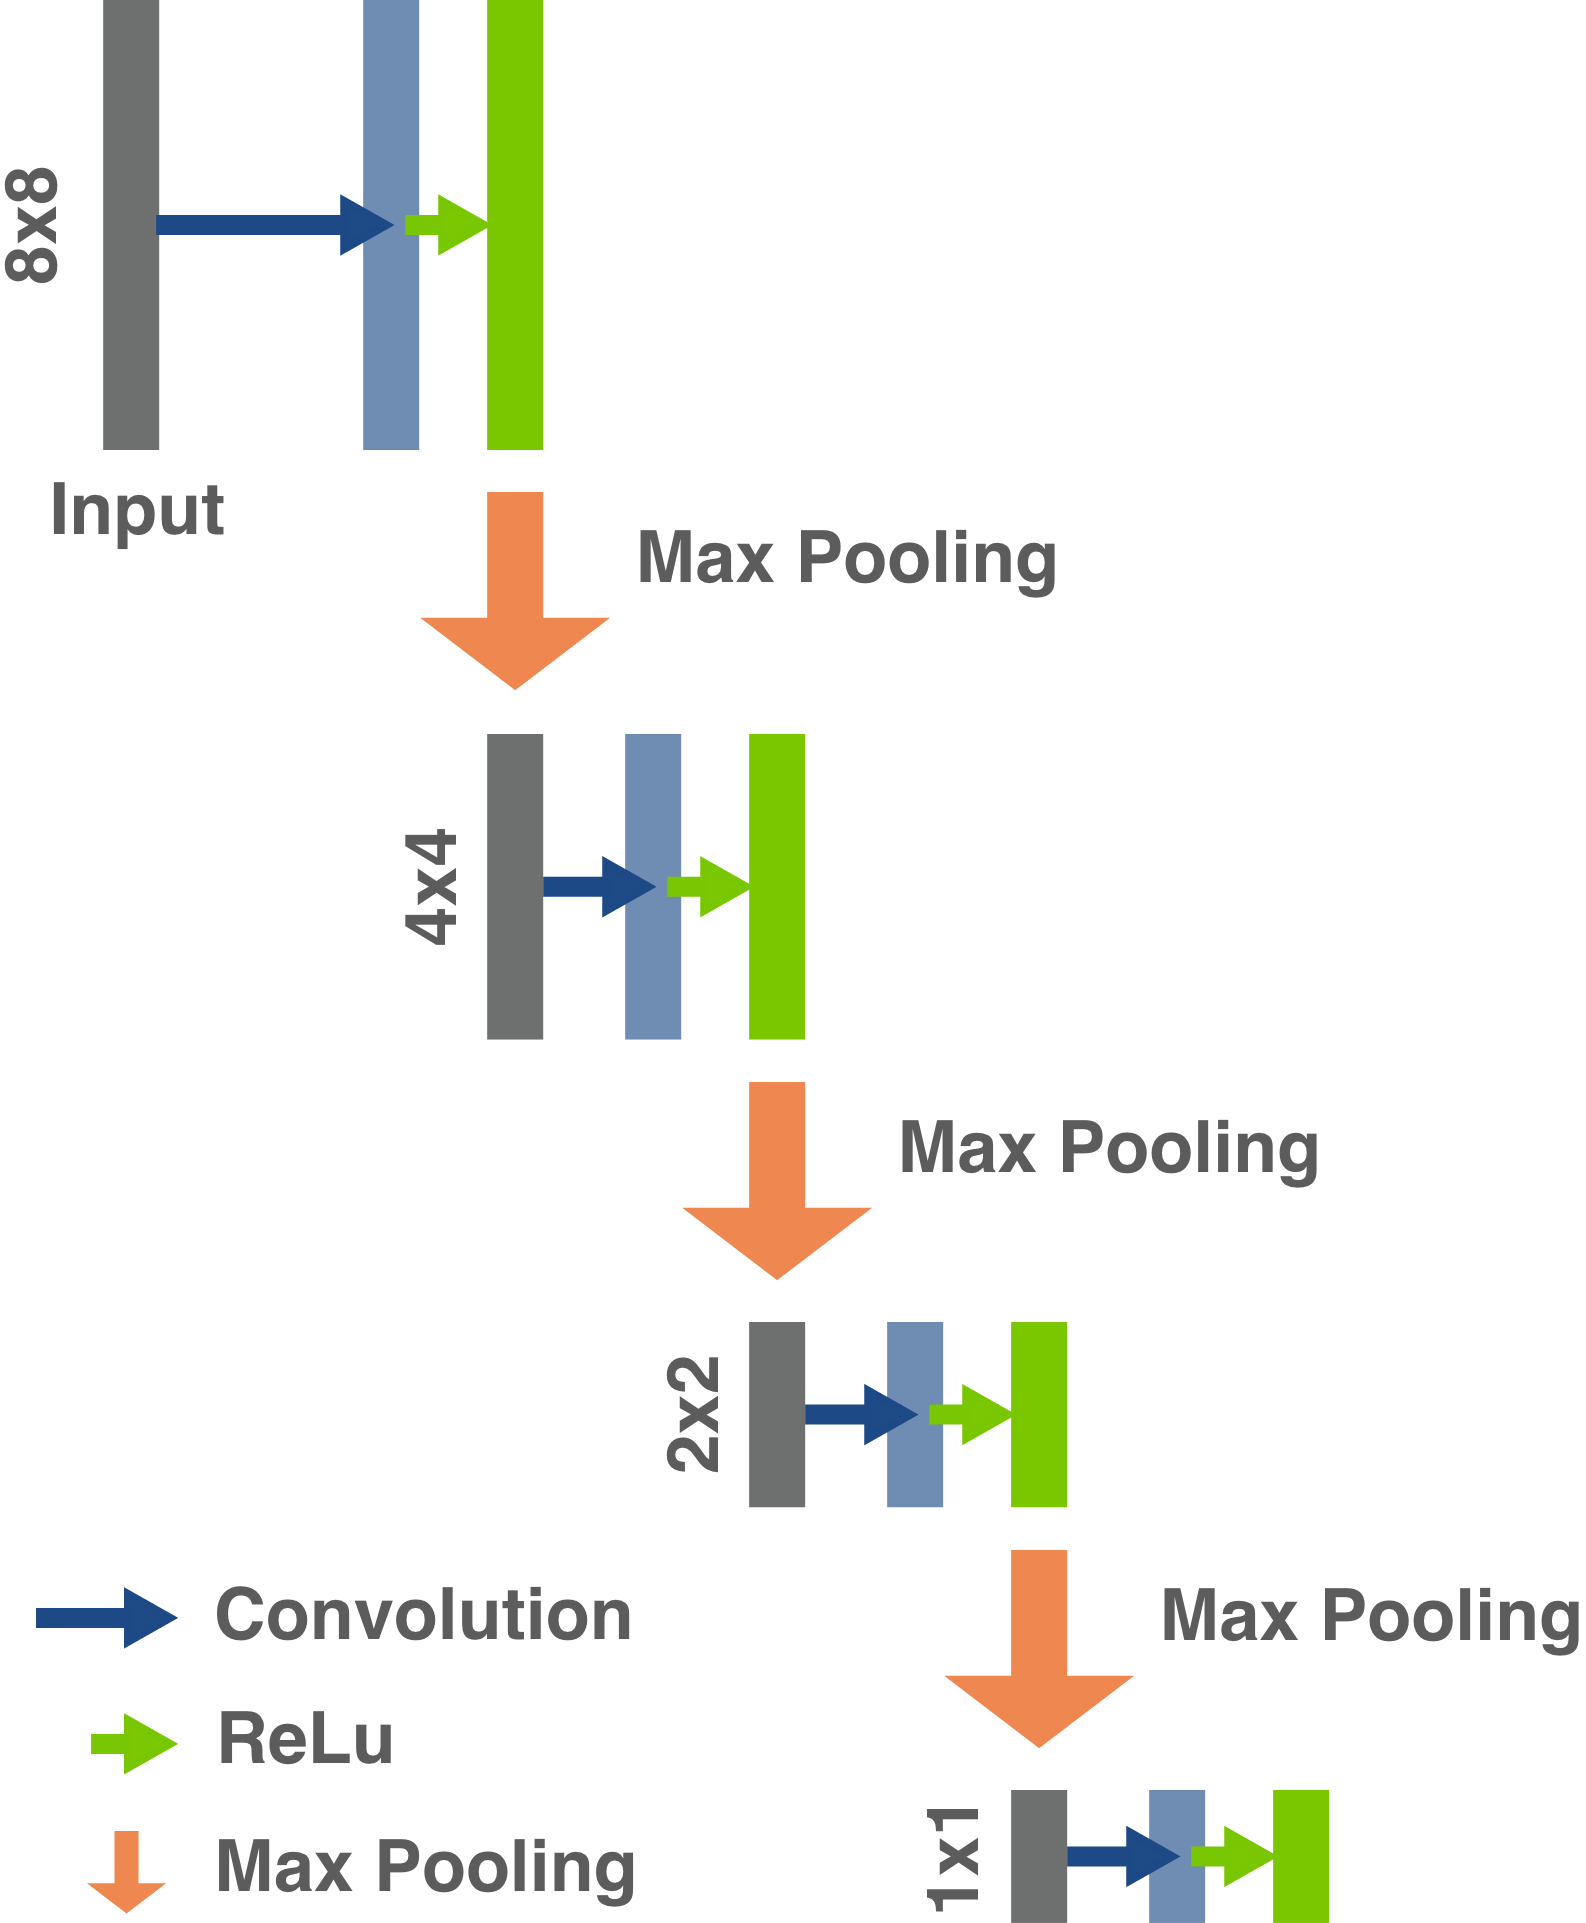
\includegraphics[width=\textwidth]{resources/images/encoder_architecture.png}
        \caption{Alternation of convolutional and pooling}
        \label{fig:encoder_architecture}
    \end{subfigure}
    \caption{Abstraction in the encoding part of a CNN.}
\end{figure}


For the 8x8 grid cells of the ERA5 data, that is used as input in the laid out approach (see \autoref{subsec:data_preprocessing}), the architecture of the CNN could include a maximum of 3 pooling layers, reducing the input data to a 1x1 matrix as seen in \autoref{fig:max_pooling}. \autoref{fig:max_pooling} just illustrates the downsampling of the data, in the actual architecture pooling layers always follow convolutional layers and are never applied directly after each other as seen in \autoref{fig:encoder_architecture}. 


\begin{figure}
    \centering
    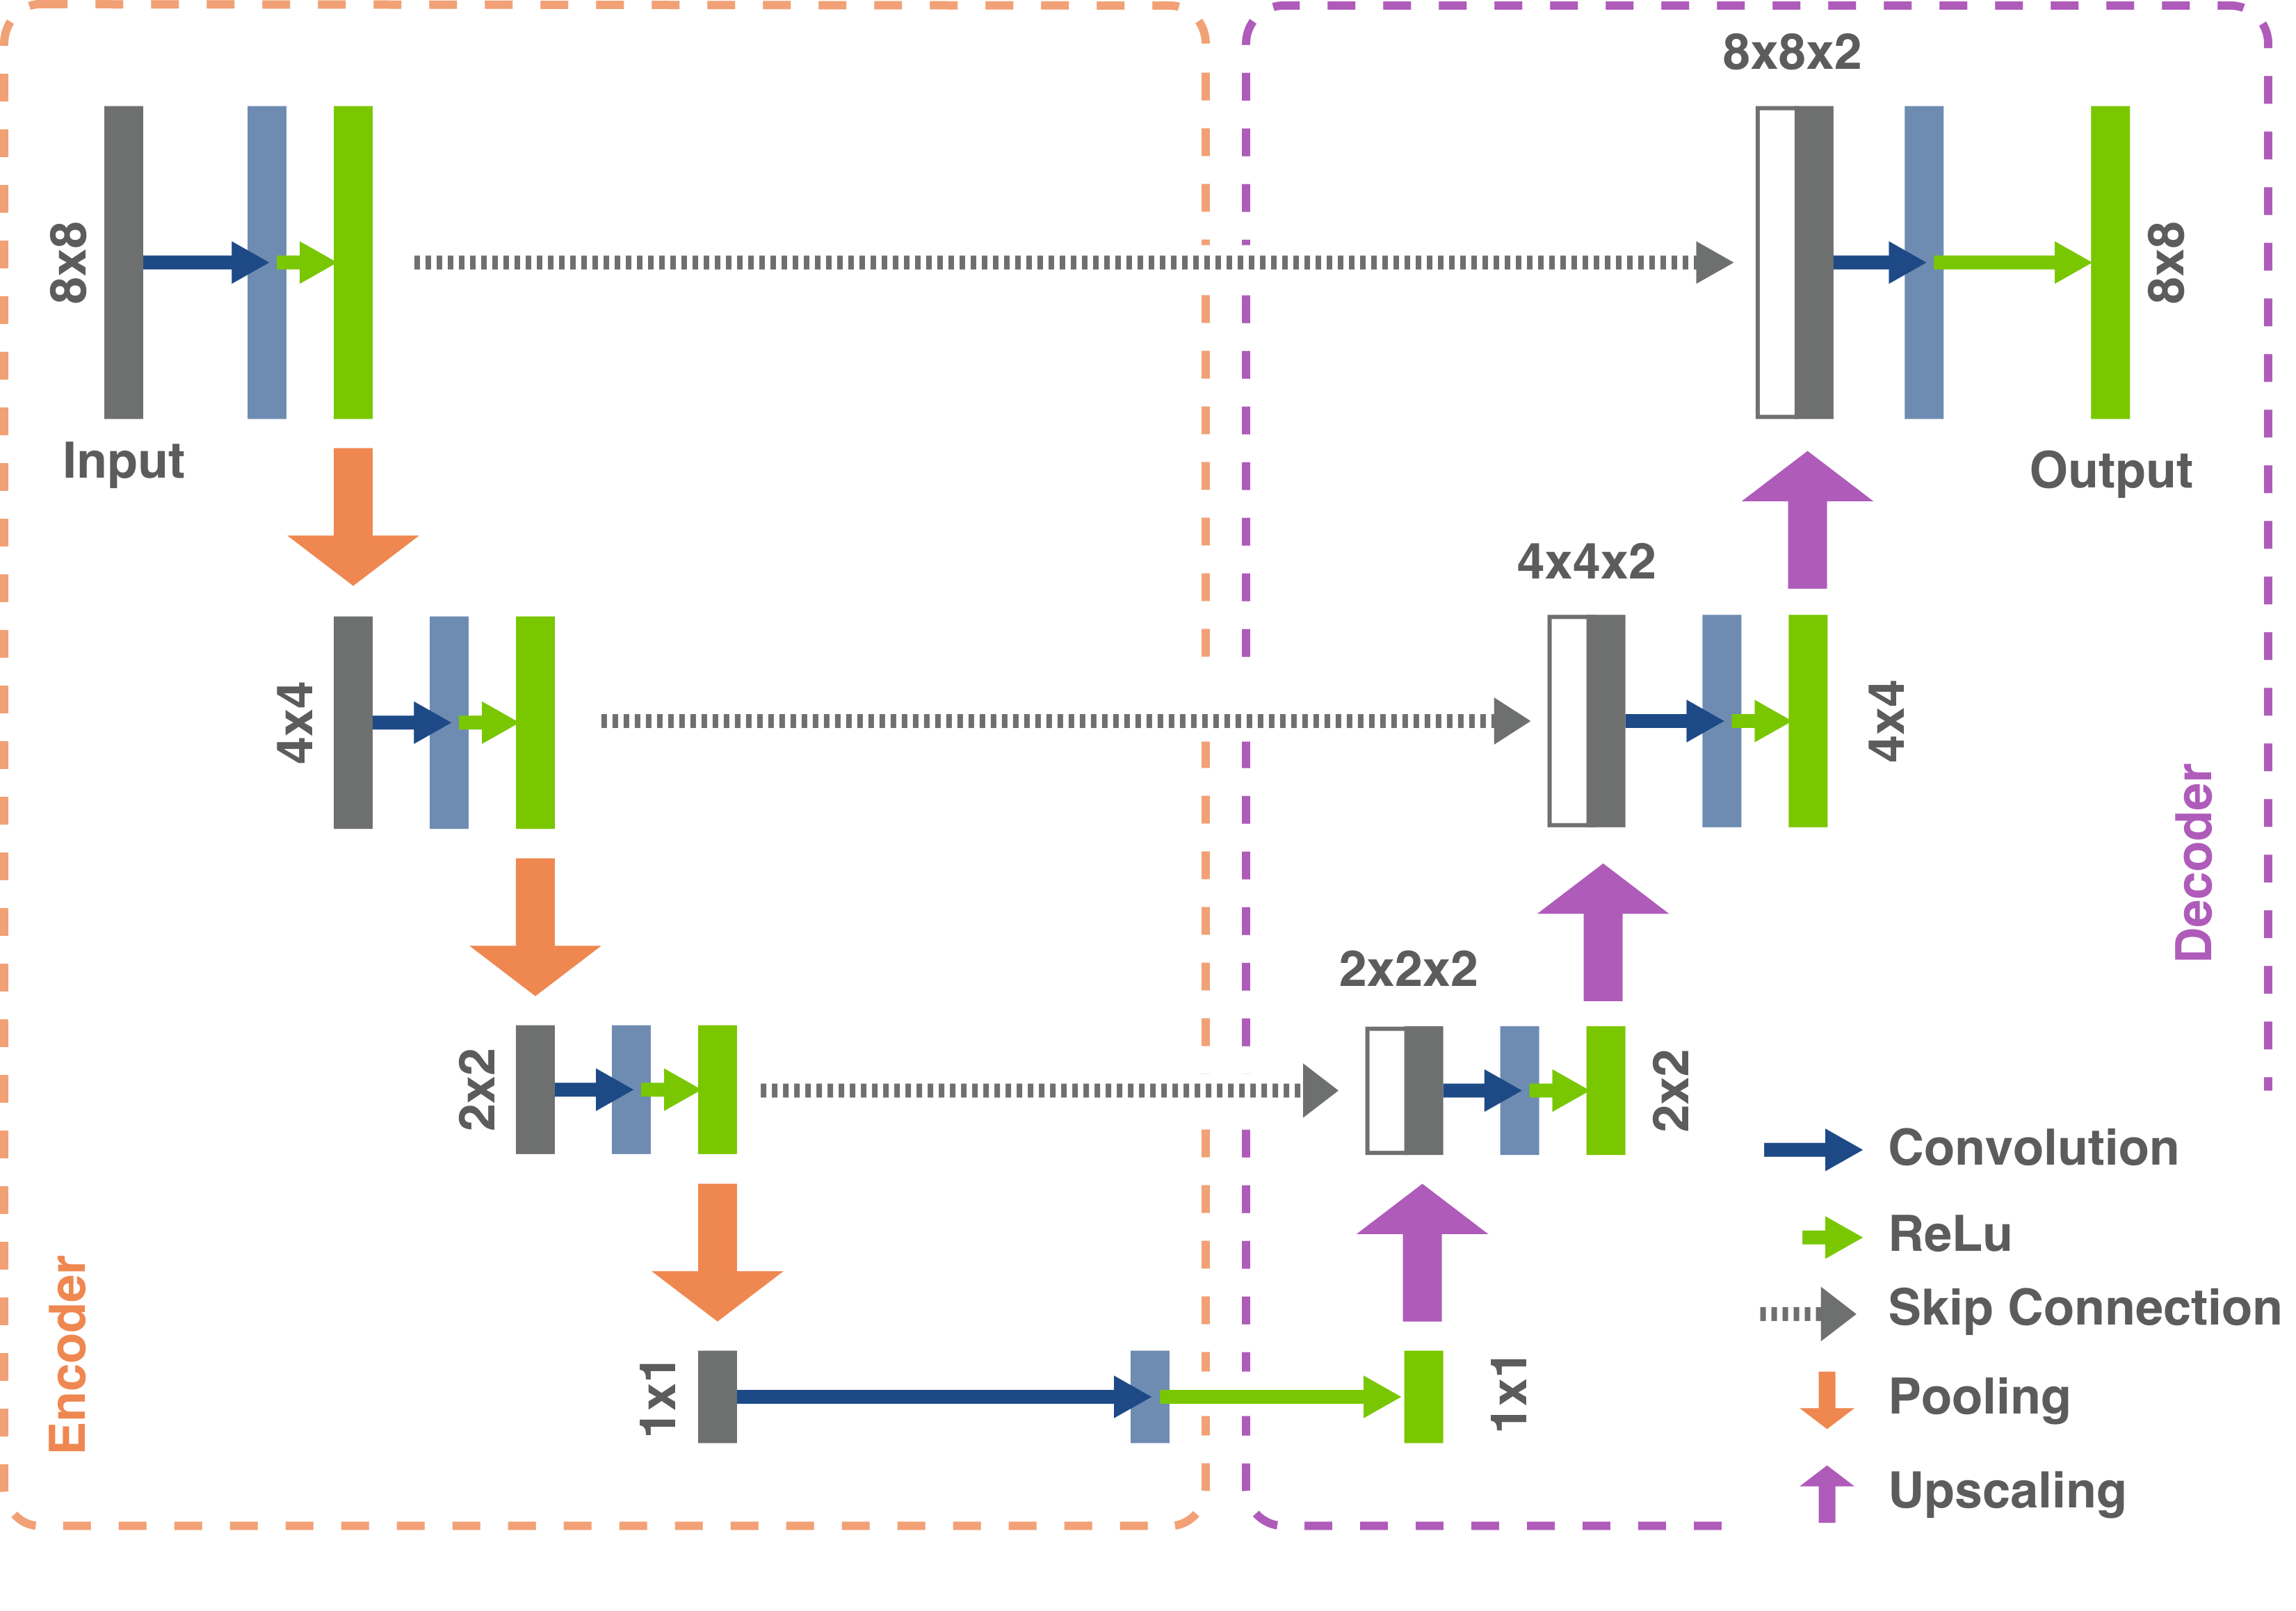
\includegraphics[width=0.9\textwidth]{resources/images/u_net.png}
    \caption{Encoder Decoder Architecture in the U-Net.}
    \label{fig:u_net}
\end{figure}

\subsubsection*{Upscaling Layer}

In the decoding part of the U-Net, the shape of the data is restored by upscaling the encoded layers with the detected feature again. This is simply done through Gaussian interpolation.

?? Question: What else can I explain here?

A very important part of the decoder is the usage of skip connections (\cite{liu2018inpaining}). 

\subsubsection*{Skip Connections}

??? Question is this even helpful when not infilling but using "target" data as input?

For the skip connections, the outputs on each layer of the encoding part are copied over and directly factored into the decoding part. This helps the network to remember the context of the input data, helping to preserve the context of the input data, which is especially important in spatial infilling tasks, where the reconstruction needs to match the available data around the missing data. To combine the data from the skip connections with the data from the upscaling layers, a specialized convolution is used... 

?? Question: Is this correct? Or Convolution->ReLU + Pooling? How is the dimensionality halved again?

The now-explained steps used in the architecture combined will return for any input data a prediction of the same shape as the input data, where the values are the predicted values for the missing data. What the values exactly will be is completely dependent on the parameters used in the convolution kernels.


?? Question: What else weights are there? The architecture does not have fully connected layers, does it? So no weights there. What about the pooling and upscaling layers? Are there weights in the activation function?

With the correct weights found the prediciton should be ideally the same as the target data. This is what the training process is for which is supervised based on the available measurements, the ground truth (see \autoref{fig:supervised_learning}). 

\subsubsection*{Backpropagation and Loss Function}

??? I am using Loss Function 3, what should I explain here in the context of a bachelor thesis about it?

To minimize any differences between ground through and prediction, the differences first need to be quantified in a loss function. Then the partial gradient of the loss function concerning each weight in the network is calculated. This is done through backpropagation, recursively applying the chain rule of calculus. The weights are then updated in the opposite direction of the gradient, such that the loss function is minimized. The learning rate determines how big the adjustments are made and is a crucial hyperparameter in the training process. 


\begin{figure}
    \centering
    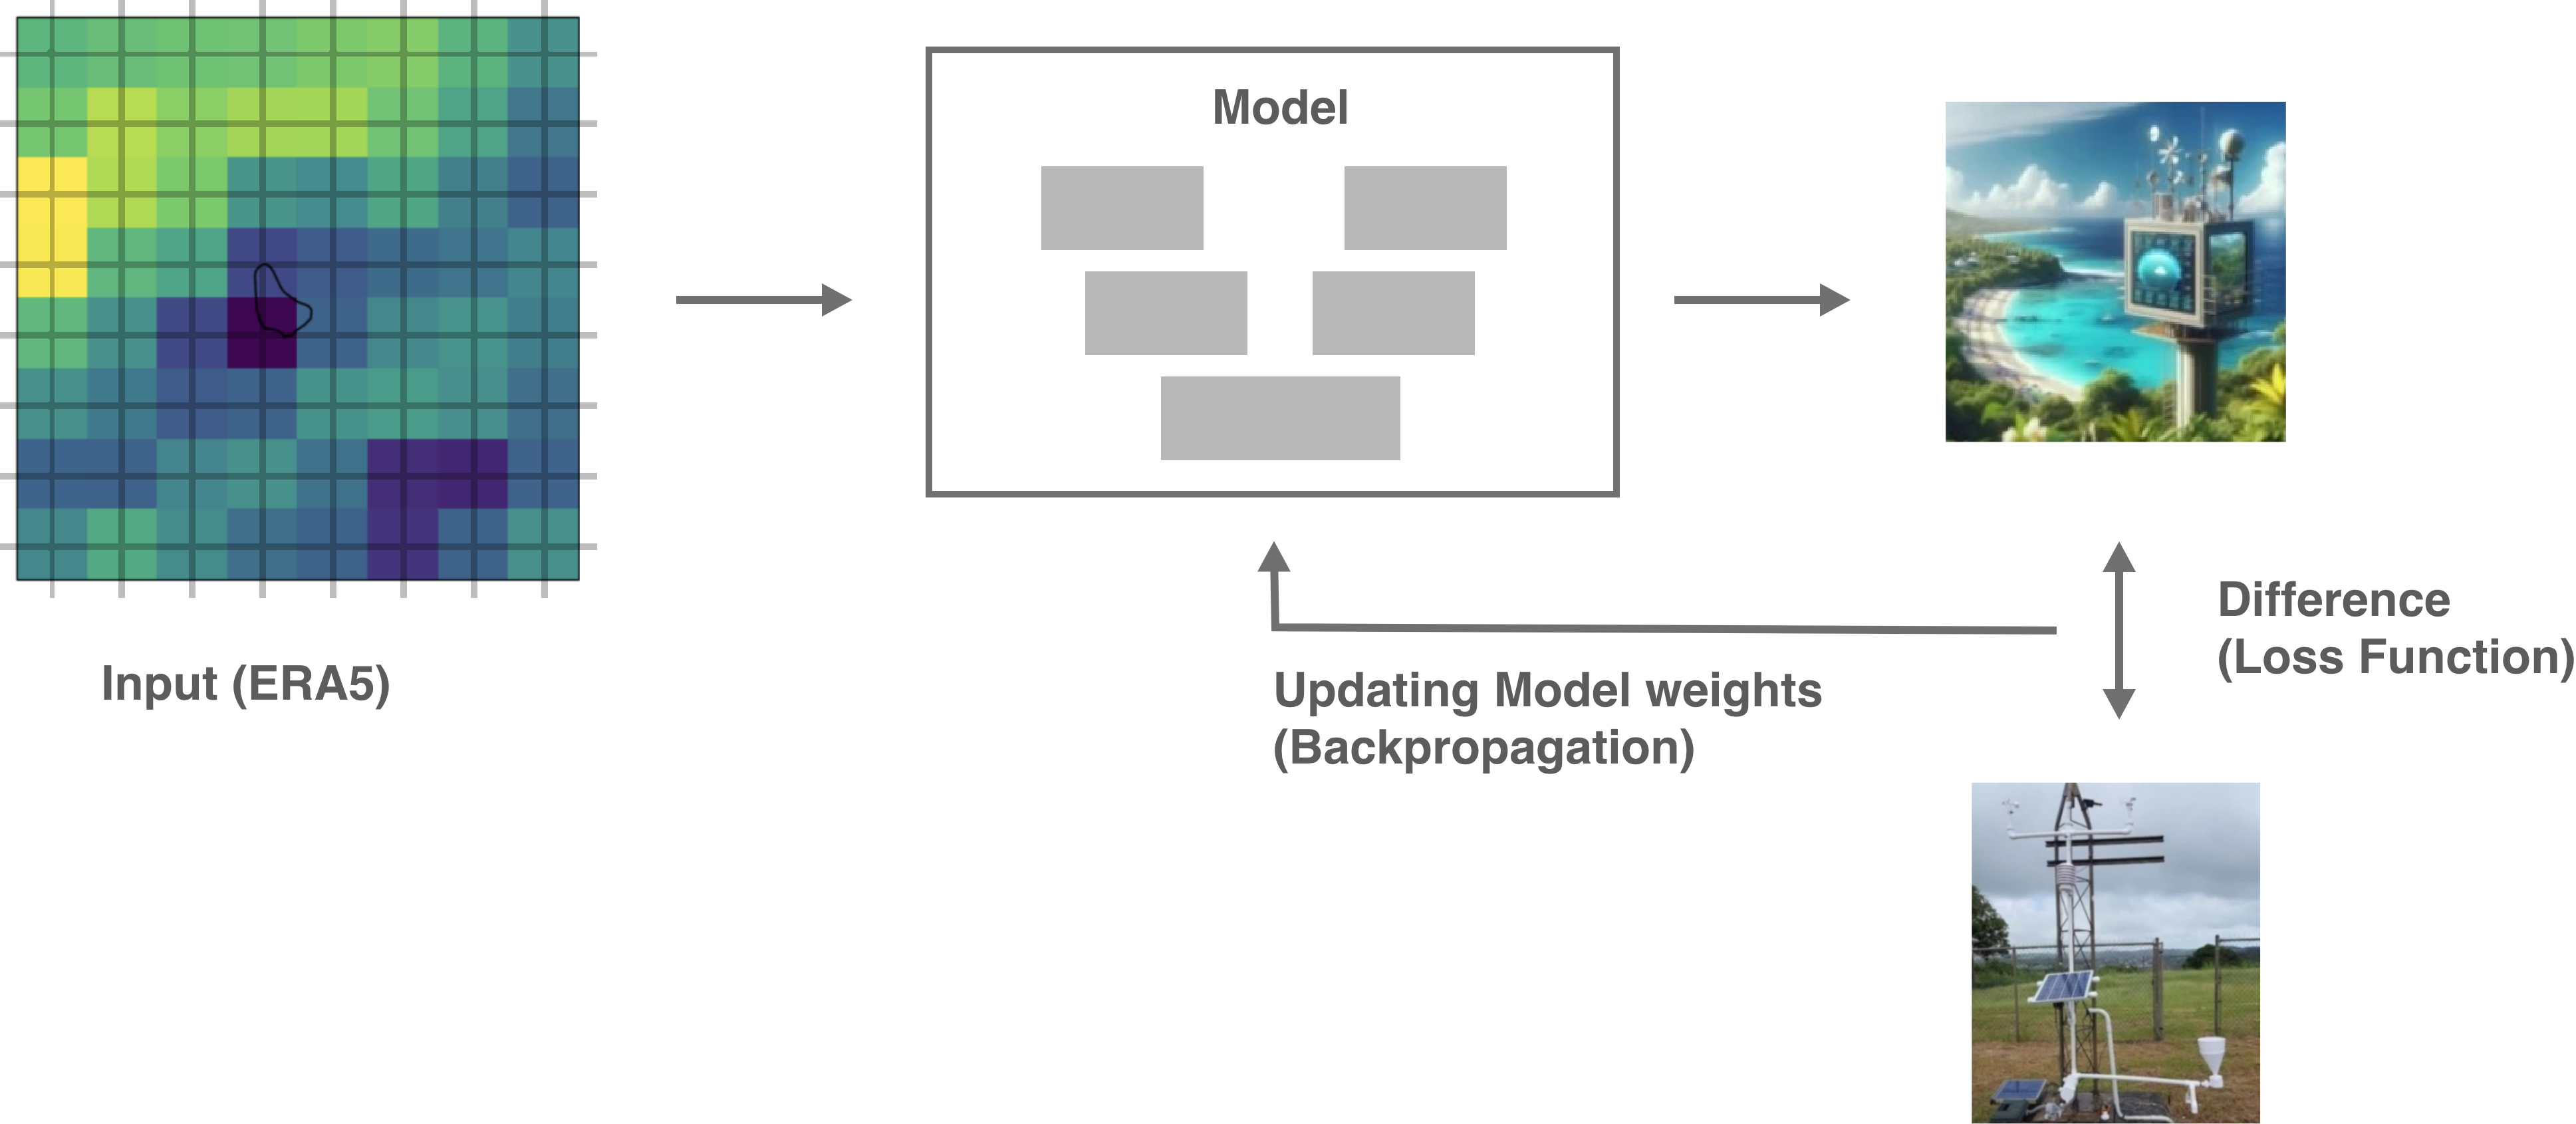
\includegraphics[width=0.9\textwidth]{resources/images/supervised_learning.png}
    \caption{Schema of supervised learning.}
    \label{fig:supervised_learning}
\end{figure}


\subsection{Reanalysis - ERA5}

Atmospheric reanalysis is an effort to combine measurements with numerical models to estimate the state of the atmosphere at any given time, opposing missing measurements. The method is based on a complex numerical model, simulating the physical rules of the atmosphere. As with any numerical model, degrees of freedom, allow for adjustments of parameters, which are chosen in such a way that the model output matches the actual measurements wherever they are available in space and time. 

The ERA5 reanalysis is a product of the European Centre for Medium-Range Weather Forecasts (ECMWF) and is the fifth generation of the ERA reanalysis series. It is the most complete and accurate data assimilation project available \cite{Hersbach2020ERA5quality}. Which makes it the best choice as input data in this approach. As it is the best available data in remote locations such as in East Africa \cite{Gleixner2020ERA5africa}, where the 3D printed weather stations are specifically supposed to make an impact it can be used as a type of benchmark to compare the results of the infilling approach to.

As mentioned above the data is available in grid cells of 0.25° x 0.25°, which is approximately 28 km x 28 km at the equator. The data assimilation takes place in 4 dimensions, as not only the latitude and longitude over time are taken into account but also multiple pressure levels in the atmosphere. This gives the techniques used for ERA5 the name 4D-Var \cite{era5}
The available variables in the ERA5 reanalysis are numerous, but for this work, only the 2m temperature is used as input to the neural network. Which is the temperature weather stations aim to measure. However, for similar approaches or extended approaches, other variables such as different wind-(component) speeds, precipitation, or humidity and solar radiation could be used as well.
% Praktischer Teil
\section{Results}
\label{sec: results}

\subsection{Included Weather Stations}

From the 3D-Paws project (see \autoref{sec: 3d_printed_stations}), measurements from three different weather stations in recent years were obtained. The stations are located in Marshall, Colorado; Vienna, Austria; and Barbados, Caribbean.

% 3 images side by side with available weather stations
\begin{figure}
\centering
\begin{subfigure}{0.672\textwidth}
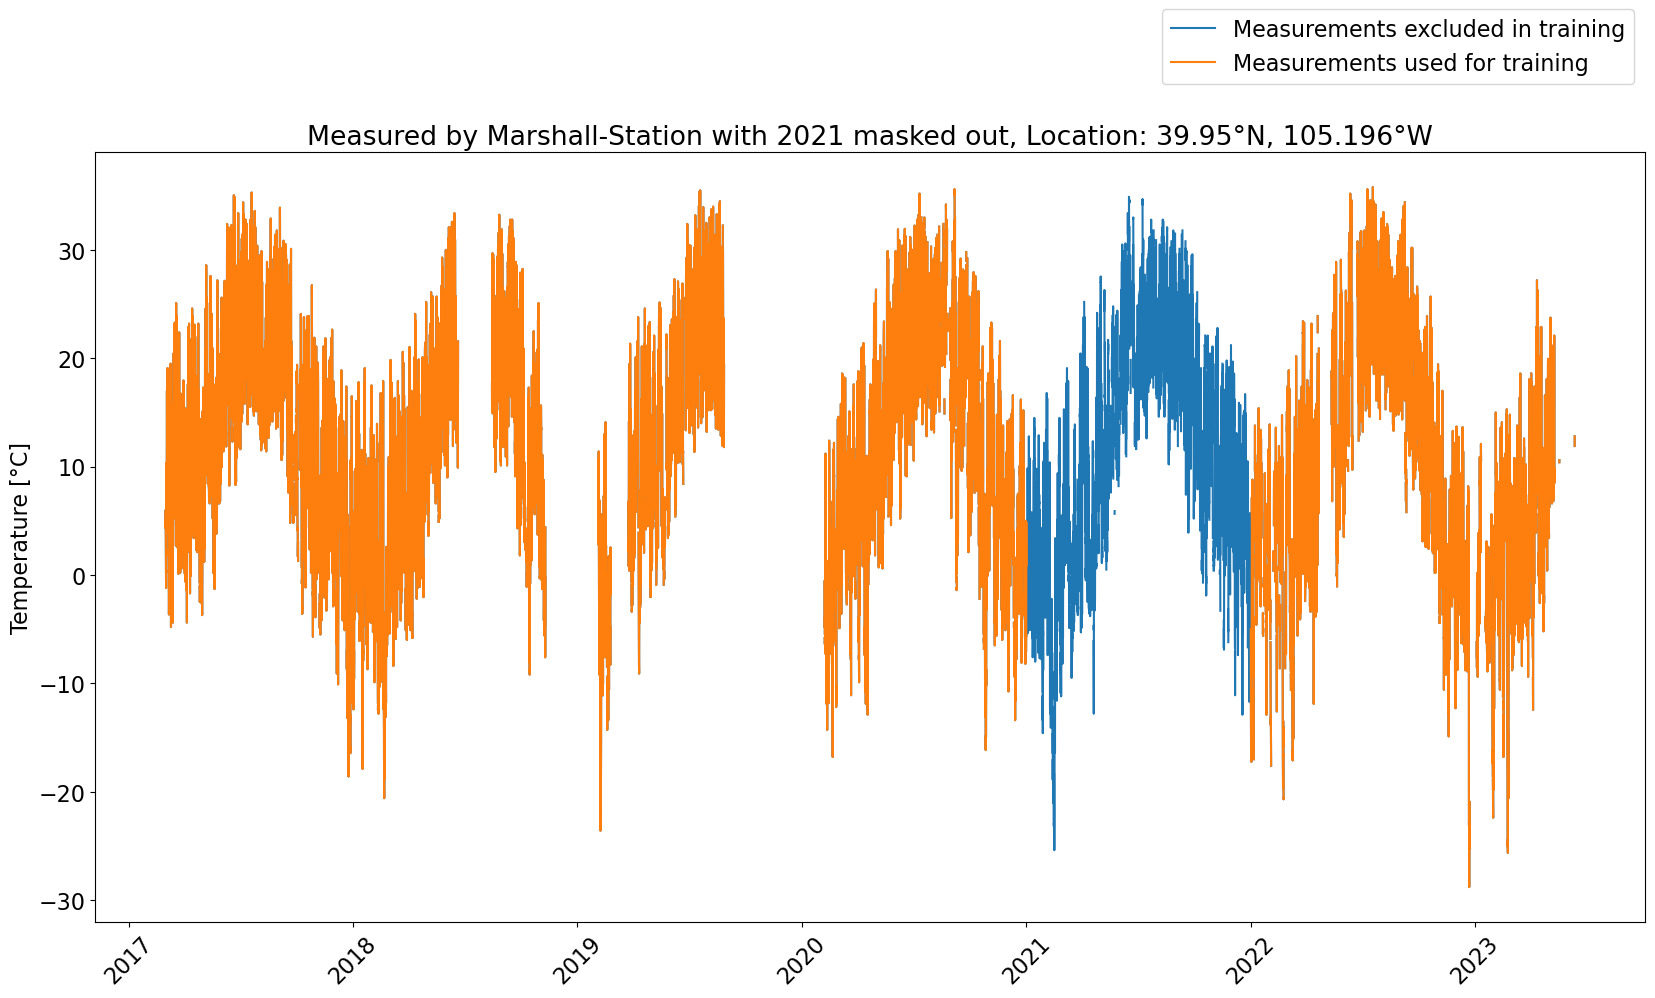
\includegraphics[width=\textwidth]{resources/images/charts/marshall_available_measurements.png}
\caption{Station in Marshall, Colorado, USA}
\label{fig: available_measurements_marshall}
\end{subfigure}
\begin{subfigure}{0.672\textwidth}
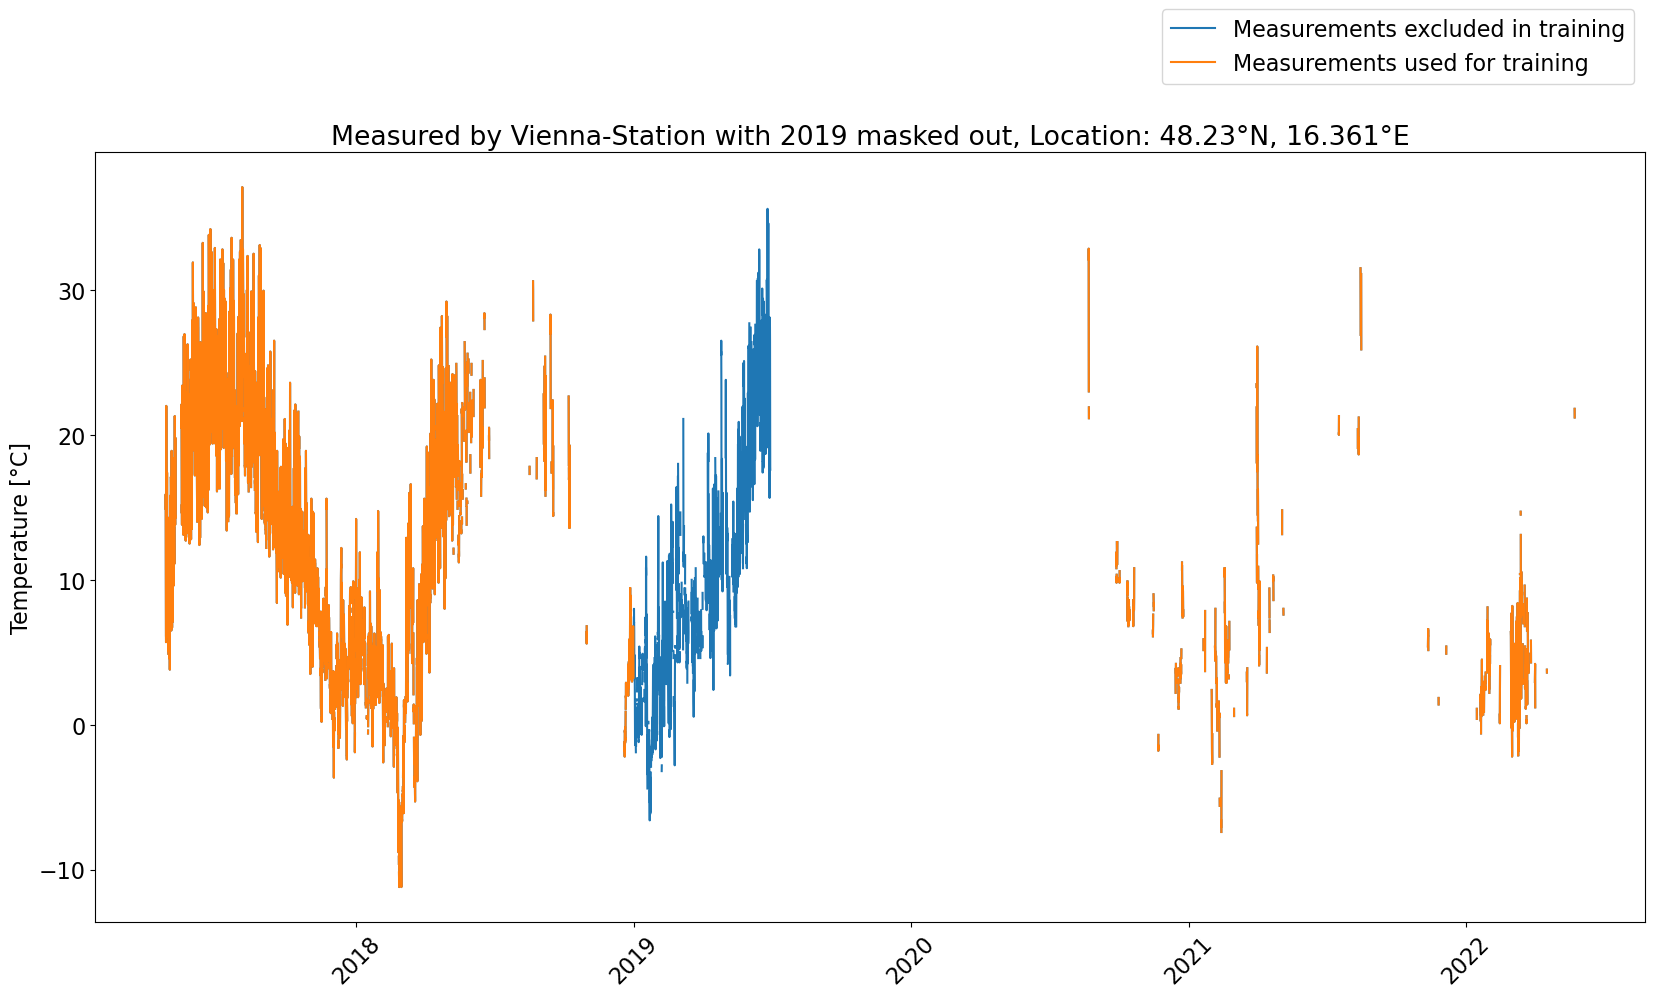
\includegraphics[width=\textwidth]{resources/images/charts/vienna_available_measurements.png}
\caption{Station in Vienna, Austria}
\label{fig: available_measurements_vienna}
\end{subfigure}
\begin{subfigure}{0.672\textwidth}
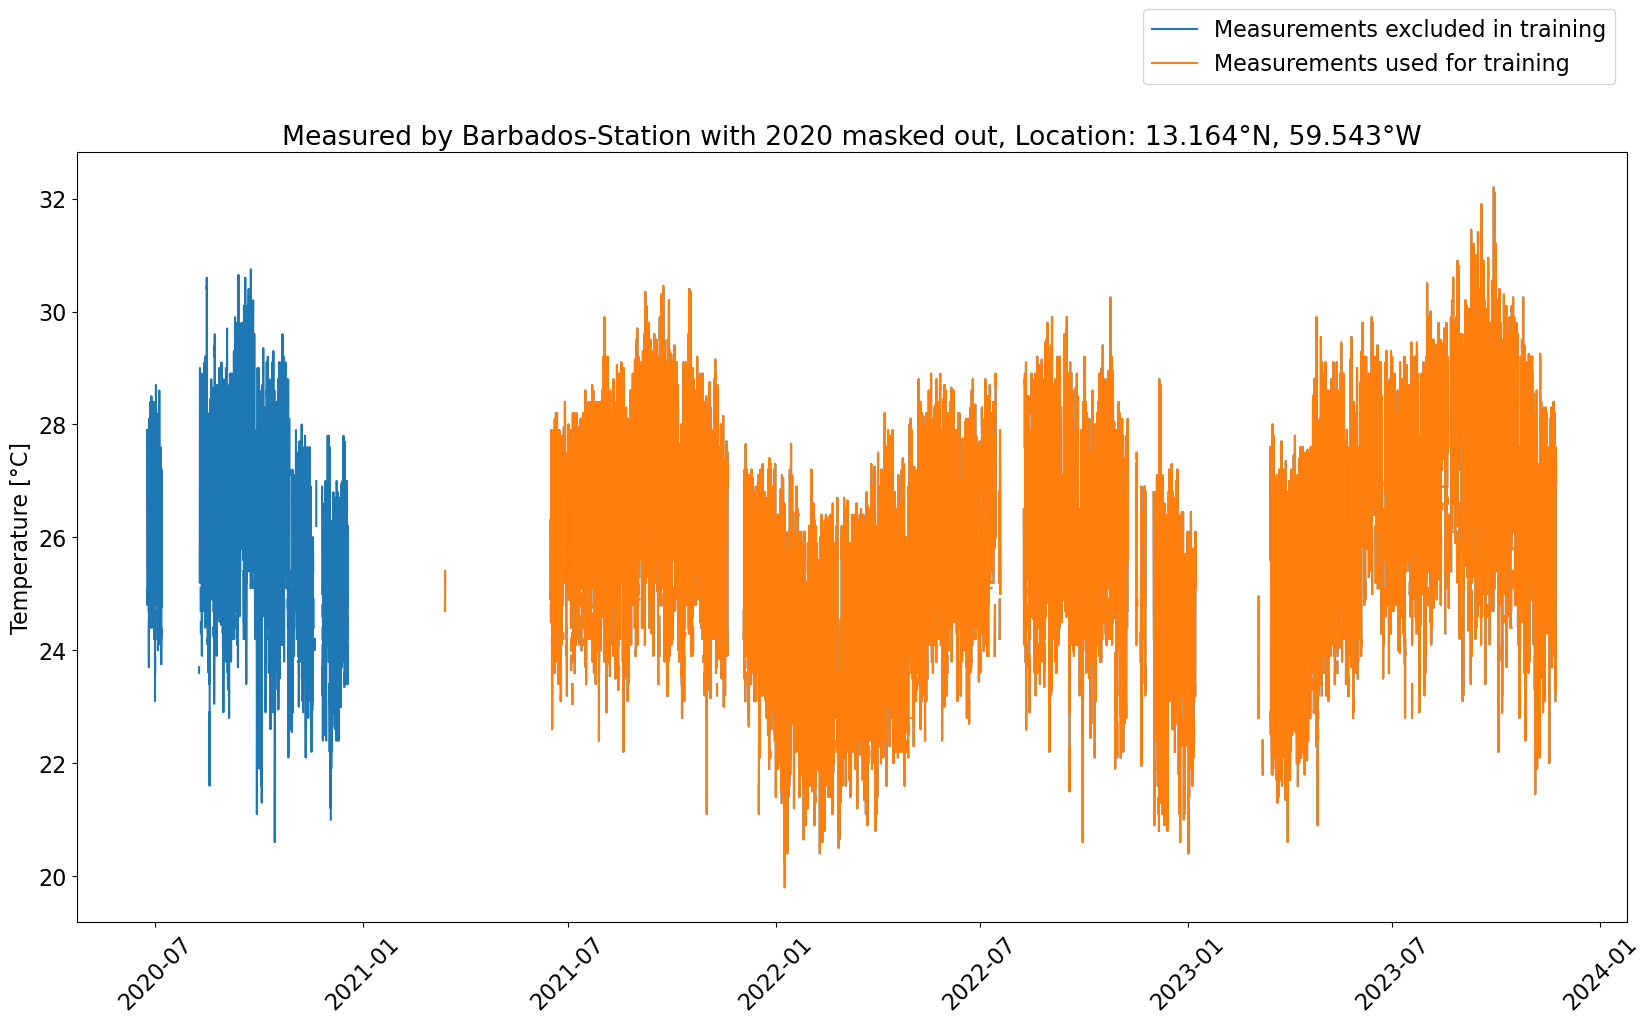
\includegraphics[width=\textwidth]{resources/images/charts/barbados_available_measurements.png}
\caption{Station in Barbados, Caribbean}
\label{fig: available_measurements_barbados}
\end{subfigure}
\caption{Available data from 3D printed Weather stations}
\label{fig: weather_stations}
\end{figure}

\begin{wrapfigure}[15]{r}{0.40\textwidth}
\centering
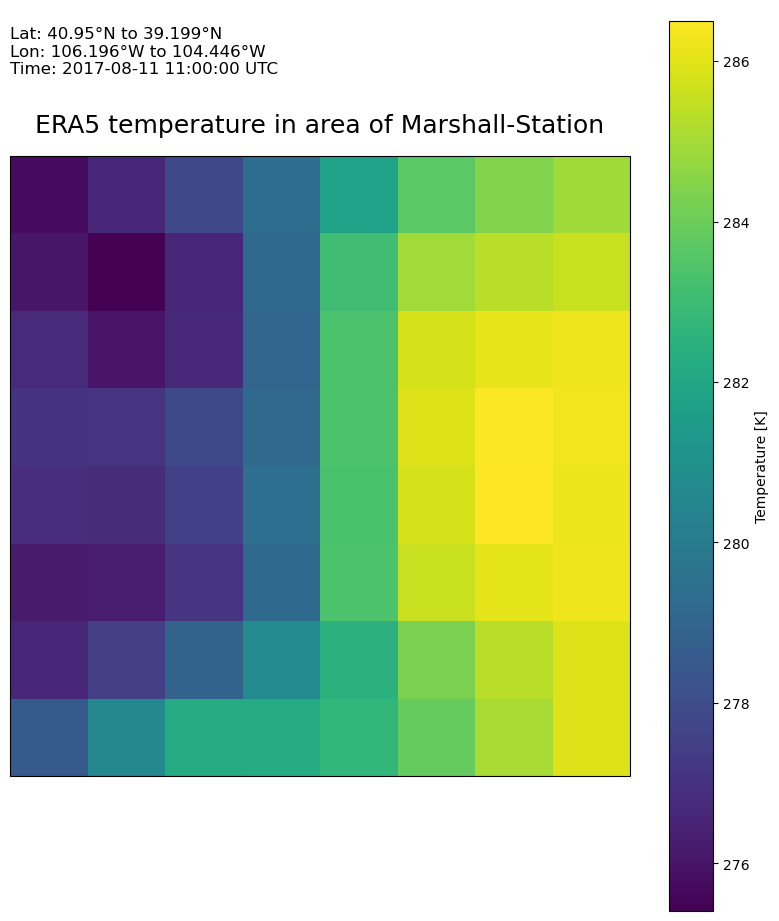
\includegraphics[width=0.38\textwidth]{resources/images/Marshall_era5.png}
\caption{ERA5 Area of the station in Marshall, Colorado}
\label{fig: era5_marshall}
\end{wrapfigure}

The station in Marshall is located between Boulder and Denver, next to Marshall Lake, at an elevation of 1,743 meters. It is less than 10 km east of South Boulder Peak, which exceeds 2,600 meters in elevation \cite{southboulderpeak}.
Further, the station is situated only about 30 km east of the Colorado Front Range, where the Rocky Mountains range in altitude between 3,250 and 4,000 meters \cite{Williams1996}.
This topographical context is visible in the ERA5 data (\autoref{fig: era5_marshall}).

Vienna lies to the west within the Vienna Basin, at a relatively low altitude just beyond the Alpine region. The Alps, which rise moderately to the west of Vienna, reach heights of up to 2,000 meters above sea level within approximately 100 km.
The ERA5 resolution is sufficient to differentiate atmospheric conditions and topographical features in this region.
The station itself resides in the north of the city on university grounds at an altitude of 159 meters.
East of it is the urban Danube Canal, separated from the station by only a main road and a railway line.

The station in Barbados stands in the parish of St. George at an altitude of 274 meters. The island is relatively flat, with its highest point being Mount Hillaby at 340 meters.
The island's size, approximately 34 km long and 23 km wide, is similar to the size of an ERA5 grid cell.
As observed in \autoref{fig: barbados}, surrounding grid cells are predominantly oceanic.
This means the ERA5 data cannot accurately capture the diurnal cycle of the station, which is influenced by its land location, while surrounding cells are mostly oceanic.

\subsection{Data Availability}

The measurements span up to late 2023, with the quantity of available temperature data varying significantly between stations. The station in Marshall, one of the oldest in the 3D-Paws project, has the most available measurements among the three stations. The weather station in Vienna has data dating back to 2017, but it has been almost entirely offline since mid-2019. The weather station in Barbados began recording in mid-2020.

\autoref{fig: weather_stations} shows the measurements from the three stations after data cleansing and conversion to an hourly basis. The measurements were provided by the US National Center for Atmospheric Research (NCAR), with most invalid values already marked. However, especially in Barbados, the sensors had more noise and occasional invalid measurements, requiring extra cleansing. Temperatures near zero and below were excluded. The conversion from minute to hourly data was done by averaging all minute values in each hour, provided there were more than 20 values available and they were not all the same. It was observed that the sensors sometimes got stuck, delivering the same value for extended periods.

The dataset for the Marshall station spans from 2017 to 2023, comprising 41,883 data points. These measurements reveal three significant data gaps, with larger intervals without data occurring in the midsummer period of 2018, late 2019 to early 2020, and the most extensive gap from September 2019 to January 2020.

For the Vienna station, measurements are available for only 12,477 hours, less than a third compared to Marshall. This is primarily due to extended downtimes starting from mid-2018, with few to no measurements except for a brief period from late 2018 to July 2019. After that, there were only sporadic data collection instances, before the station went offline in April 2022.

The Barbados station had two significant downtimes longer than a month, the largest being the first half of 2021 and the second being the first quarter of 2023. In total, the station has 17,315 hours of measurements, still less than half of the Marshall station.

\subsubsection*{Splitting into Training and Validation Data}

As explained in \autoref{sec: design}, the measurements are split into a training and validation dataset. The training dataset is used to train the model, while the validation dataset will be kept aside to compare it to what the model predicts after the training to validate if and to which extent the model learned to reconstruct the missing data. If the validation data would be included in the training data, the model would be able to predict the values it has already seen, but it would be impossible to tell if the model learned to generalize the local weather patterns.
Starting with the Marshall station, the data was sufficient to extract an entire year as validation data. Excluding a consecutive year from the training data not only allows for a comprehensive analysis of a full yearly cycle but also ensures that the model relies solely on the general weather patterns it learned from the training data to predict the values of the validation data. This approach prevents the model from potentially "cheating" by accessing information from nearby training data points, which could compromise the integrity of the validation process. It is a common practice in the machine learning field to validate data as a contiguous set, as it helps to maintain the independence and integrity of the validation process. 2021 highlighted in blue in \ref{fig: available_measurements_marshall} was the most complete year in the Marshall dataset thus it was chosen as the validation data. With the mask of 2021 applied the training data for Marshall consists of 34,188 hours of measurements which is about 82\% of the total data.

For the Vienna station, the data was split into training and validation data based on the availability of the data. The training data consists of all available data up to 2019, while the validation data is the year 2019. Resulting in 9,593 hours of measurements used as training data, which is about 77\% of the total data. The limited availability of measurements didn't allow for a full year of validation data.

The Barbados station also only had 2022 and 2023 as a complete available years, so that the decision to use the available data of 2020 as a training was a result of the lack of data as well. With the mask applied, the training data consists of 14,576 hours of measurements, which is about 84\% of the total data.


% Marshall 41883, 34188 without 2021 -> gives a ratio for validation data of 0.18

% Barbados 17315, 14576 without 2020 -> gives a ratio for validation data of 0.16

% Vienna 12477, 9593 without 2019 -> gives a ratio for validation data of 0.23

%Table with the data availability and the split into training and validation data

\begin{table}
\centering
\begin{tabular}{|c|c|c|c|c|}
\hline
Station & Total Data & Training Data & Validation Data & Validation Ratio \\
\hline
Marshall & 41,883 & 34,188 & 7,695 & 0.18 \\
Barbados & 17,315 & 14,576 & 2,739 & 0.16 \\
Vienna & 12,477 & 9,593 & 2,884 & 0.23 \\
\hline
\end{tabular}
\caption{Data availability and split into training and validation data}
\label{tab:data_split}
\end{table}

\subsubsection*{Execution of Training}

For the training and validation data, the corresponding temperature data of the 64 ERA5 grid cells in the regions of each station was obtained.
The 8x8 grid cells were chosen to be centered as well as possible around each weather station, given the specific ERA5 coordinates.
The ERA5 data was also preprocessed using the code pipeline described in \autoref{sec: implementation}.
Then, the CNN with the architecture described in \autoref{subsec:cnn} was trained on the training data. The training was done in batches of 4 data points, which are, in hour case, the hourly steps at a time. The model was trained for up to 300,000 iterations, which, therefore, depend on the dataset size between 8 and 31 epochs. The training was done on the Supercomputer "Levante" of the German Climate Computing Center, which made it possible to complete training runs in just a few hours. However, the training can be done in the same way on almost any machine. During the training, in the scientific process, where the approach is un-proven to work, it is especially important to validate multiple times during the training to calculate not only the loss function over the model for the training data, but over the validation data. This is done to prevent overfitting, a so-called phenomenon where the model in the aim to minimize the loss for the training data, which is what training using backpropagation is exactly at it is core, starts to learn the noise and any potential specifics of the training data so well, that it loses it is ability to generalize and the loss for the validation data starts to increase. This is a sign that the model is overfitting and the training should be stopped. The model that is then chosen is the one that performed best on the validation data. To allow for that, not only was the ERA5 data for the training data provided to the machine learning architecture but the validation ERA5 data was also paired with the expected output for these, the masked measurements of the weather station.

Training runs have been completed for all stations with up to 1 million iterations, but the best models were in most cases, already found between 300 and 500 thousand iterations. The models were then applied to the ERA5 data at all the hours in the validation data set of each station, to analyze the performance of the model for each station. 

\subsection{Validation Methods}

As numerical measures of quality, the Root Mean Squared Error (RMSE) and the correlation coefficient were calculated.
RMSE quantifies proximity between two series in terms of distance (refer to \autoref*{fig: low_rmse}), yet it lacks insight into their trend relationship.
Conversely, the correlation coefficient gauges the model's fidelity to the overall trend of the observed data (as depicted in \autoref*{fig: high_corr}).
Notably, high correlation can coexist with significant distance between series.

\begin{figure}
    \centering
    \begin{subfigure}{0.35\textwidth}
        \centering
        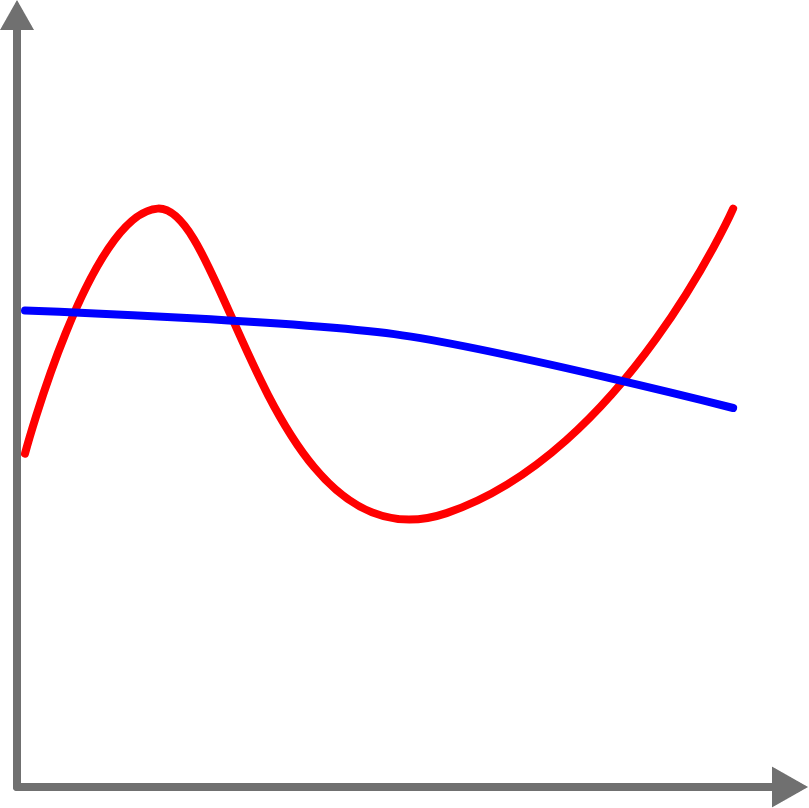
\includegraphics[width=0.7\textwidth]{resources/images/low_rmse.png}
        \caption{Low RMSE, low Correlation Coefficient}
        \label{fig: low_rmse}
    \end{subfigure}
    \hspace{0.5cm}
    \begin{subfigure}{0.35\textwidth}
        \centering
        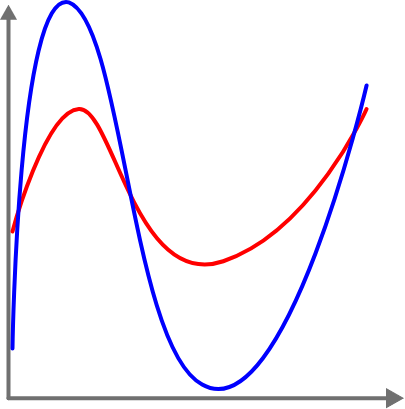
\includegraphics[width=0.7\textwidth]{resources/images/high_corr.png}
        \caption{High Correlation Coefficient, high RMSE}
        \label{fig: high_corr}
    \end{subfigure}
    \caption{Comparison of the RMSE and Correlation Coefficient}
\end{figure}

\subsubsection*{Root Mean Squared Error (RMSE)}

To quantify how far apart the reconstructed temperature series $\hat{y}$ is from the measured temperature series $y$, where both series have $n$ different timesteps and thus can be seen as vectors, most commonly the root mean squared error (RMSE) comes to help, which is strongly connected to the Euclidean norm of the difference between both vectors $\hat{y} - y$. However, a simple mean absolute error (MAE), also called the Manhattan norm, could seem most intuitive and easiest to understand. It would be calculated just by adding all absolute differences up before dividing it by the length of the series. The RMSE is favored in machine learning and statistics because it penalizes larger differences more than smaller ones, which is more in line with the human perception of errors. 

\begin{equation}
    \text{RMSE} = \sqrt{\frac{1}{n} \sum_{i=1}^{n} (y_i - \hat{y}_i)^2}
    \label{eq: rmse}
\end{equation}

\begin{equation}
    \text{MAE} = \frac{1}{n} \sum_{i=1}^{n} |y_i - \hat{y}_i|
    \label{eq: mae}
\end{equation}

When converting \autoref*{eq: rmse}, it can be seen how the RMSE is connected to the Euclidean norm:

\begin{equation}
  \text{RMSE} \cdot \sqrt{n} = \sqrt{\sum_{i=1}^{n} (y_i - \hat{y}_i)^2} = \| y - \hat{y} \|_2  
  \label{eq: rmse_euclid}
\end{equation}

The Euclidean norm $\| y - \hat{y} \|_2$, of a coordinate in our case the error $\hat{y} - y$ can be imagined as the diagonal distance between the origin and the point with these coordinates. For demonstration purposes, a right triangle in 2-dimensional space can be imagined with the errors at 2 validation timesteps as the legs. The RMSE over both errors would be proportional to the hypothenuse of that triangle which is more dependent on the length of the longer leg than the shorter one. The Manhattan norm (\autoref{eq: mae}), on the other hand, which received its name from the gridded street system of Manhattan is not based on the diagonal distance, but the distance a taxicab in Manhattan would have to drive to travel along the hypothenuse, the equally weighted sum of the legs.

\subsubsection*{Pearson Correlation Coefficient}

The Pearson correlation coefficient (in the following called correlation coefficient), is a measure of the strength and direction of a linear relationship between two variables. It ranges from -1 to 1, where 1 indicates a perfect positive linear relationship, -1 is a perfect negative linear relationship, and 0 is no linear relationship. The correlation coefficient is calculated as follows:

\begin{equation}
    \text{Correlation Coefficient} = \frac{\sum_{i=1}^{n} (y_i - \bar{y})(\hat{y}_i - \bar{\hat{y}})}{\sqrt{\sum_{i=1}^{n} (y_i - \bar{y})^2 \sum_{i=1}^{n} (\hat{y}_i - \bar{\hat{y}})^2}}
    \label{eq: correlation}
\end{equation}
    
Where $\bar{y}$ and $\bar{\hat{y}}$ are the mean values of the measured and the model output temperature series, respectively. The correlation coefficient is a measure of how well the model output follows the general trend of the measured data. \cite{Zou2003Correlation}

\subsection{Validation of the Models}

\subsubsection*{Marshall-Station}

\begin{figure}
    \centering
    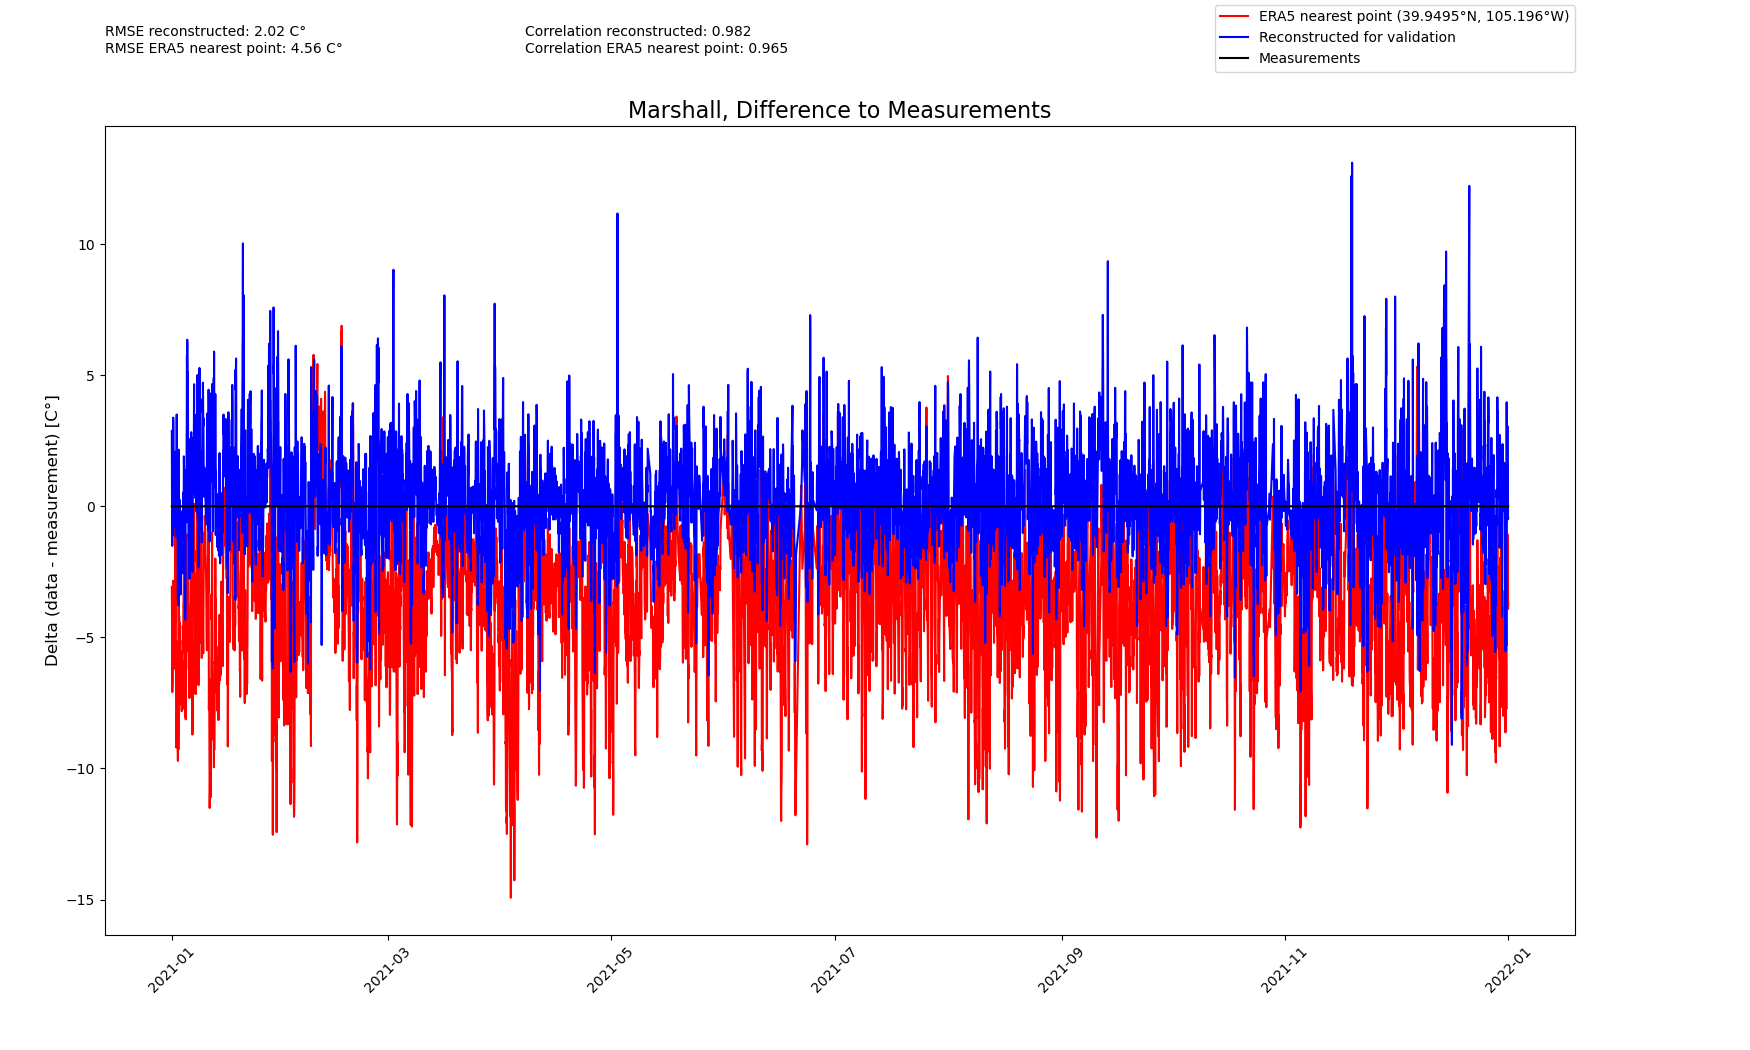
\includegraphics[width=1.00\textwidth]{resources/images/charts/marshall_eval_grib_final/Marshall, Difference to Measurements.png}
    \caption{Difference between reconstructed and measured hourly temperature for Marshall-Station}
    \label{fig: marshall_diff}
\end{figure}
% RMSE reconstructed: 2.02, RMSE ERA5: 4.56, Correlation reconstructed: 0.982, Correlation ERA5: 0.965
% ERA5 has a low bias

To begin with Marshall the occasion with the most available training data, all by the model predicted temperatures for the hourly measurements of the validation dataset have been plotted in \autoref{fig: marshall_diff} with a blue line against the ground truth in black. Given the high number of hourly timesteps along the x-axis spanning the year 2021, for the sake of readability, the temperature differentials are plotted on the y-axis instead of the absolute temperatures.
Above the chart the over the whole hourly validation data calculated RMSE and Correlation of the reconstructed series are written.
The RMSE for the Marshall station is 2.02°C, which is the highest value among the three weather stations.
To compare the RMSE to what a direct read out of ERA5 would have been, the plot includes in red the temperature at each timestep at the nearest ERA5 grid point, at the coordinates 39.950° N, 106.196° W. The grid point's location is exactly the location of the weather station in Marshall (see \autoref{fig: available_measurements_marshall}).
But the RMSE between the measurements and the temperature time series of that ERA5 grid point, is 4.56°C, which is more than twice as high.
Considering that the model was trained on the ERA5 data of the 8x8 grid cells around the station, the model was able to reduce the error significantly.
The ERA5 data, as seen in the chart has a substantial low-bias compared to the station which directly relates to the fact that the grid cell of the station already reaches into the Rocky Mountains, as described above.
Thus it is especially important, that the reconstruction not just has a lower RMSE which could be achieved in this case just by correcting the low-bias but also beats it is training data in terms of correlation.
The calculated correlation coefficient over the validation year 2021 on an hourly basis for the reconstructed temperature and the measurements is 0.982 compared to 0.965 for the ERA5 nearest grid point a significant improvement.

\begin{figure}
    \centering
    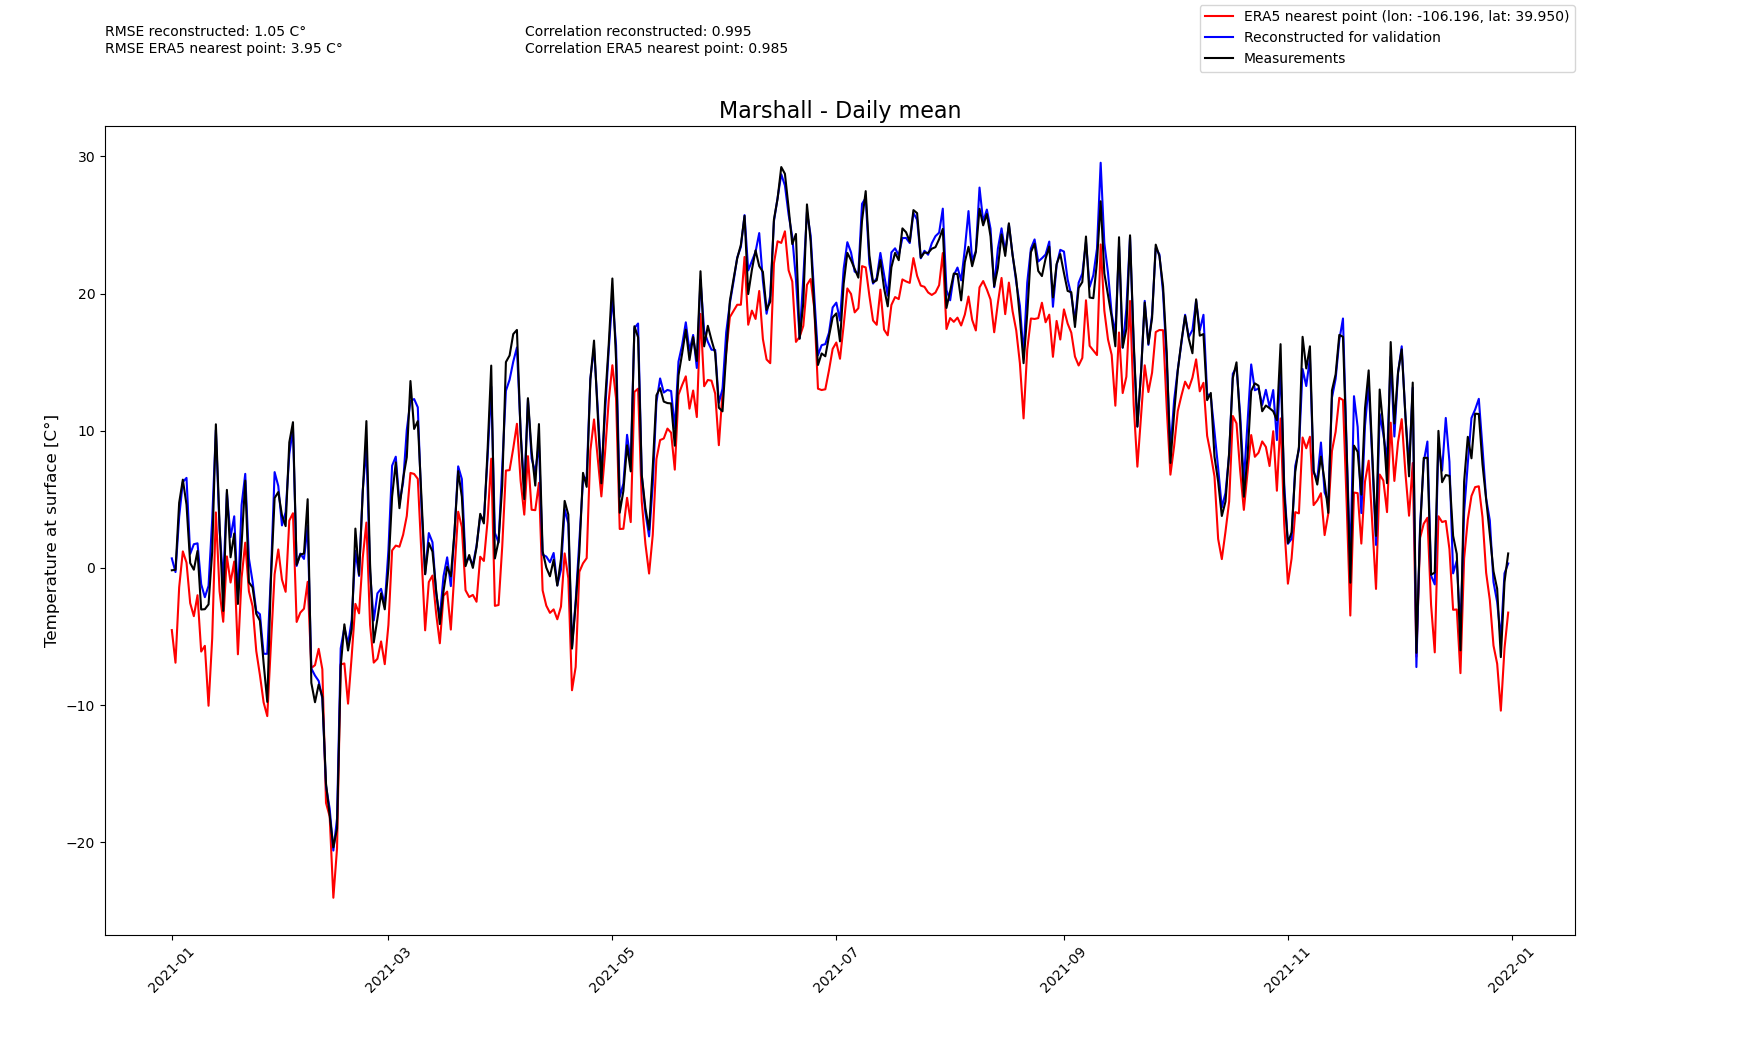
\includegraphics[width=1.00\textwidth]{resources/images/charts/marshall_eval_grib_final/Marshall - Daily mean.png}
    \caption{Reconstructed temperature vs measured temperature for Marshall-Station (Daily mean)}
    \label{fig: marshall_daily}
\end{figure}
% RMSE reconstructed: 1.05, RMSE ERA5: 2.02, Correlation reconstructed: 0.995, Correlation ERA5: 0.982
% ERA5 has a low bias

Even better is the performance of the model when the hourly values are combined again with daily means, as in \autoref{fig: marshall_daily}.
The chart shows the daily mean temperature of the three different series, known from the previous chart over 2021. In this case, the reduced number of timesteps allows for an absolute temperature scale on the y-axis and therefore makes the performance of the model visually appealing as well, the RMSE on a daily basis for the prediction is almost halved the original one at 1.05°C, while the correlation coefficient is even higher as well at 0.995, the ERA5 correlation coefficient improved significantly as well, however, the RMSE didn't as the ERA5 data is impacted drastically by the low-bias.

\begin{figure}
    \centering
    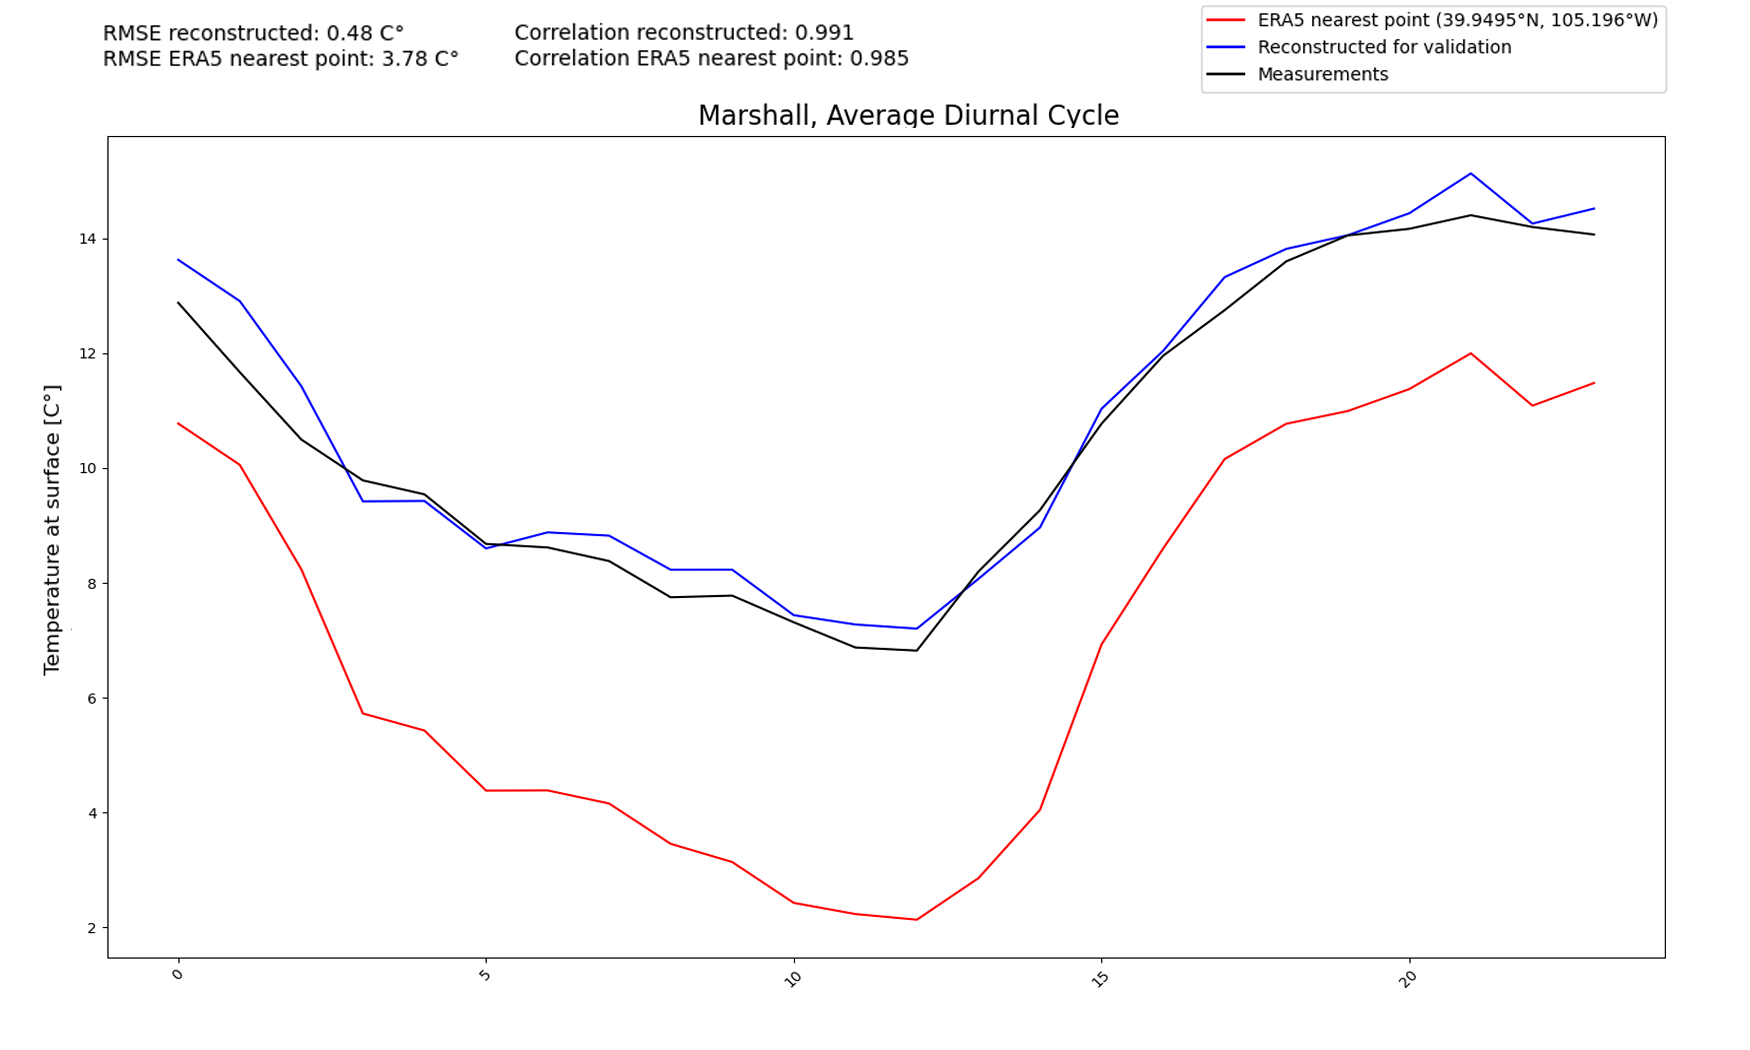
\includegraphics[width=1.00\textwidth]{resources/images/charts/marshall_eval_grib_final/Marshall, Average Diurnal Cycle.png}
    \caption{Reconstructed temperature vs measured temperature for Marshall-Station (Average Diurnal Cycle)}
    \label{fig: marshall_diurnal}
\end{figure}
% RMSE reconstructed 0.48, RMSE ERA5 3.78, Correlation reconstructed 0.991, Correlation ERA5 0.985

\autoref{fig: marshall_diurnal} makes clear, that the improvement in RMSE and correlation coefficient of the daily analysis was not caused by potential issues in the model to predict the diurnal cycle correctly but by noise reduction in general.
In \autoref{fig: marshall_diurnal} the average diurnal cycle of the reconstructed temperature is plotted against the measured temperature and the temperature series of ERA5.
This means that over all the days in 2021, for each of the 24 hours, an average temperature was calculated and plotted for the three series.
As all measurements, have been recorded in universal time code (UTC), which is also the time in ERA5, the x-axis is also using UTC, which is apart from the daylight savings time 6 hours ahead of Colorado.
It can be observed that ERA5 has a higher amplitude in the diurnal cycle than the weather station and that the model is capable of correcting that.

It is not surprising, that the RMSE and correlation coefficient improve the more the data is aggregated, so it is also important to look at the hourly values again and go into detail. To allow the details to appear on a plot, the x-axis can be cropped to a shorter period, as in \autoref{fig: marshall_7day}, where the x-axis includes 168 hours, equivalent to 7 days.
The chart is chosen to be representative, while some weeks have a better fitting than others. In this case, it can be seen, that even in the measurements of 2021, minor gaps happened. For example  


\begin{figure}
    \centering
    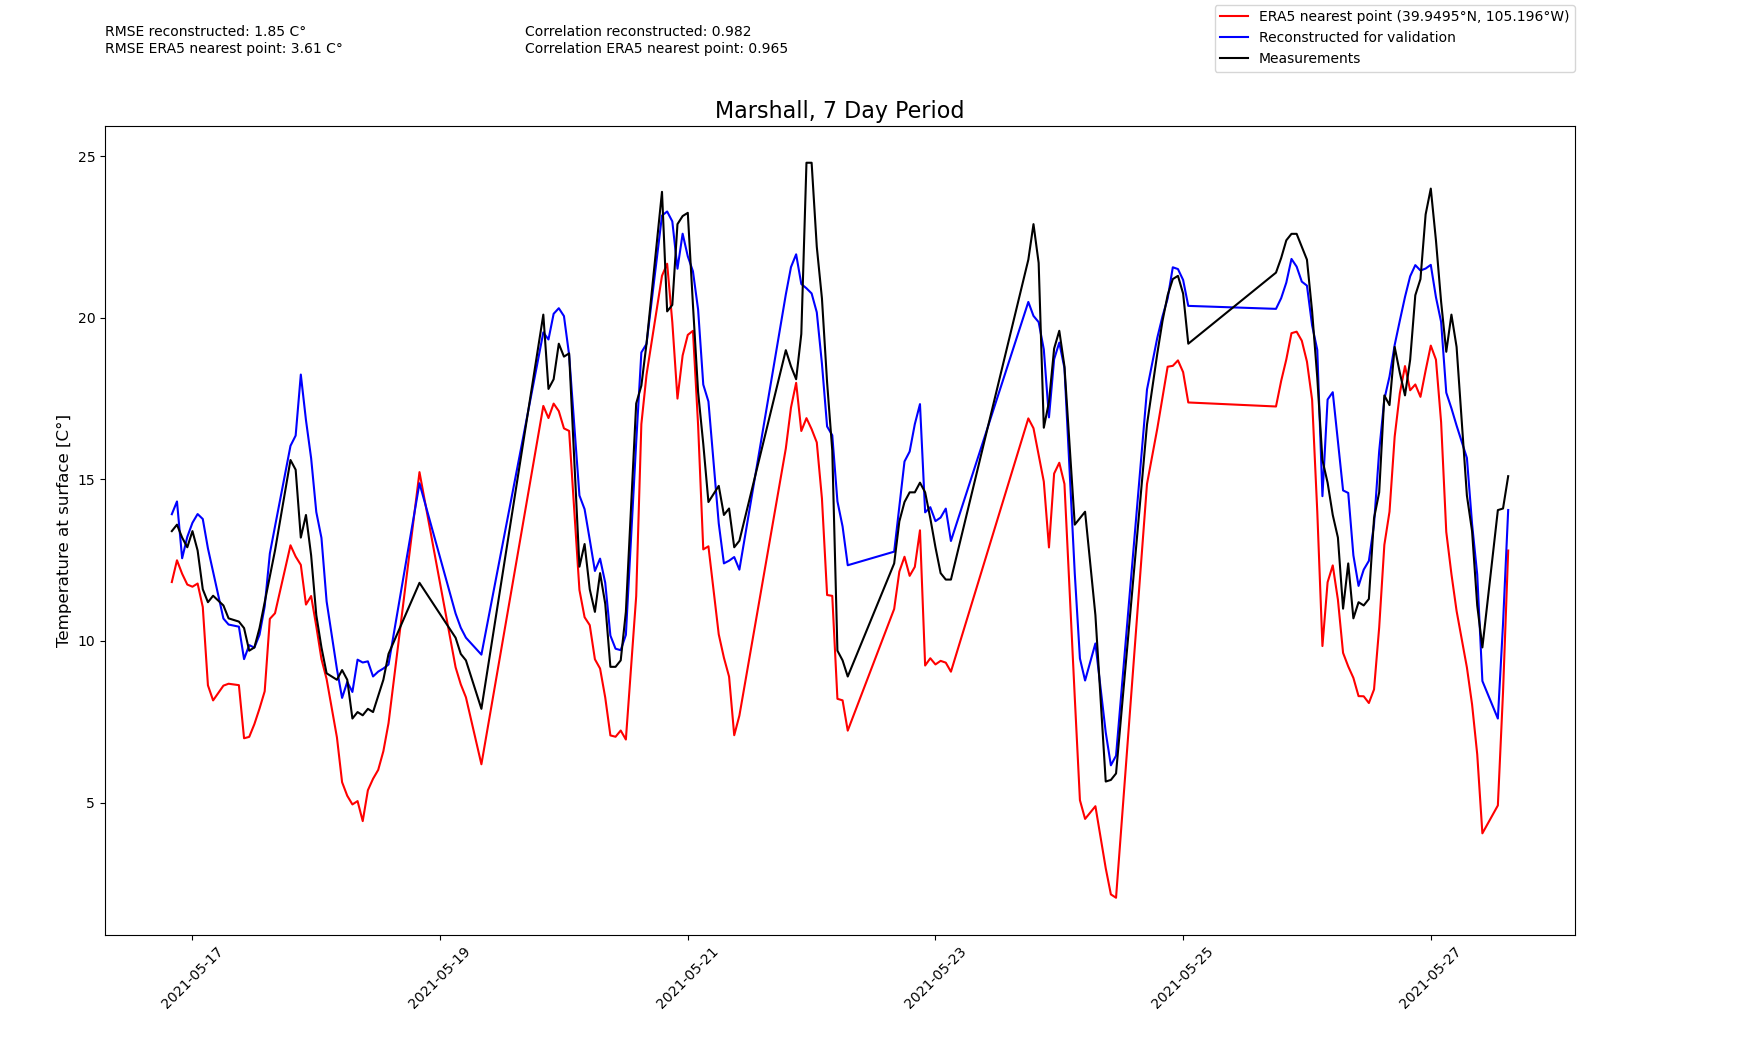
\includegraphics[width=1.00\textwidth]{resources/images/charts/marshall_eval_grib_final/Marshall, 7 Day Period_1_2_3.png}
    \caption{Reconstructed temperature vs measured hourly temperature for Marshall-Station (7 Day Period)}
    \label{fig: marshall_7day}
\end{figure}

\begin{figure}
    \centering
    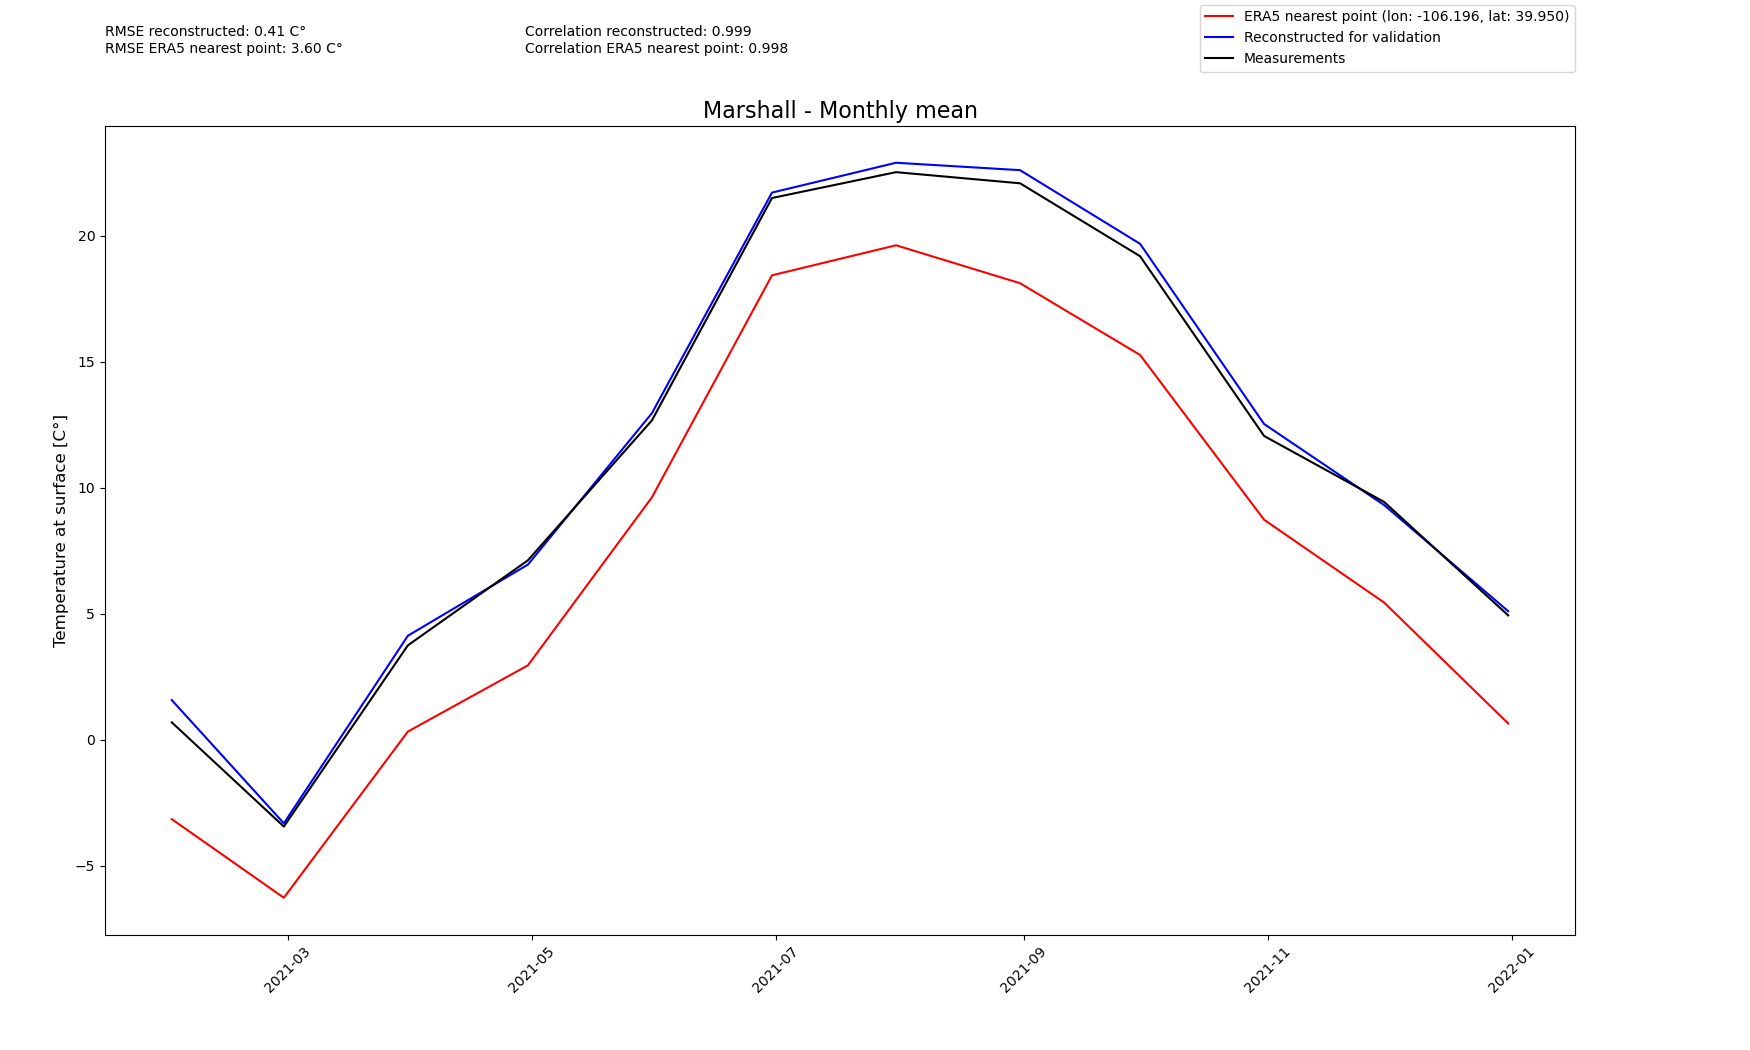
\includegraphics[width=1.00\textwidth]{resources/images/charts/marshall_eval_grib_final/Marshall - Monthly mean.png}
    \caption{Reconstructed temperature vs measured temperature for Marshall-Station (Monthly mean)}
\end{figure}
% RMSE reconstructed 0.41, RMSE ERA5 3.60, Correlation reconstructed 0.999, Correlation ERA5 0.998
% super good result but of course monthly means...

\subsection{Vienna-Station}
\begin{figure}[H]
\centering
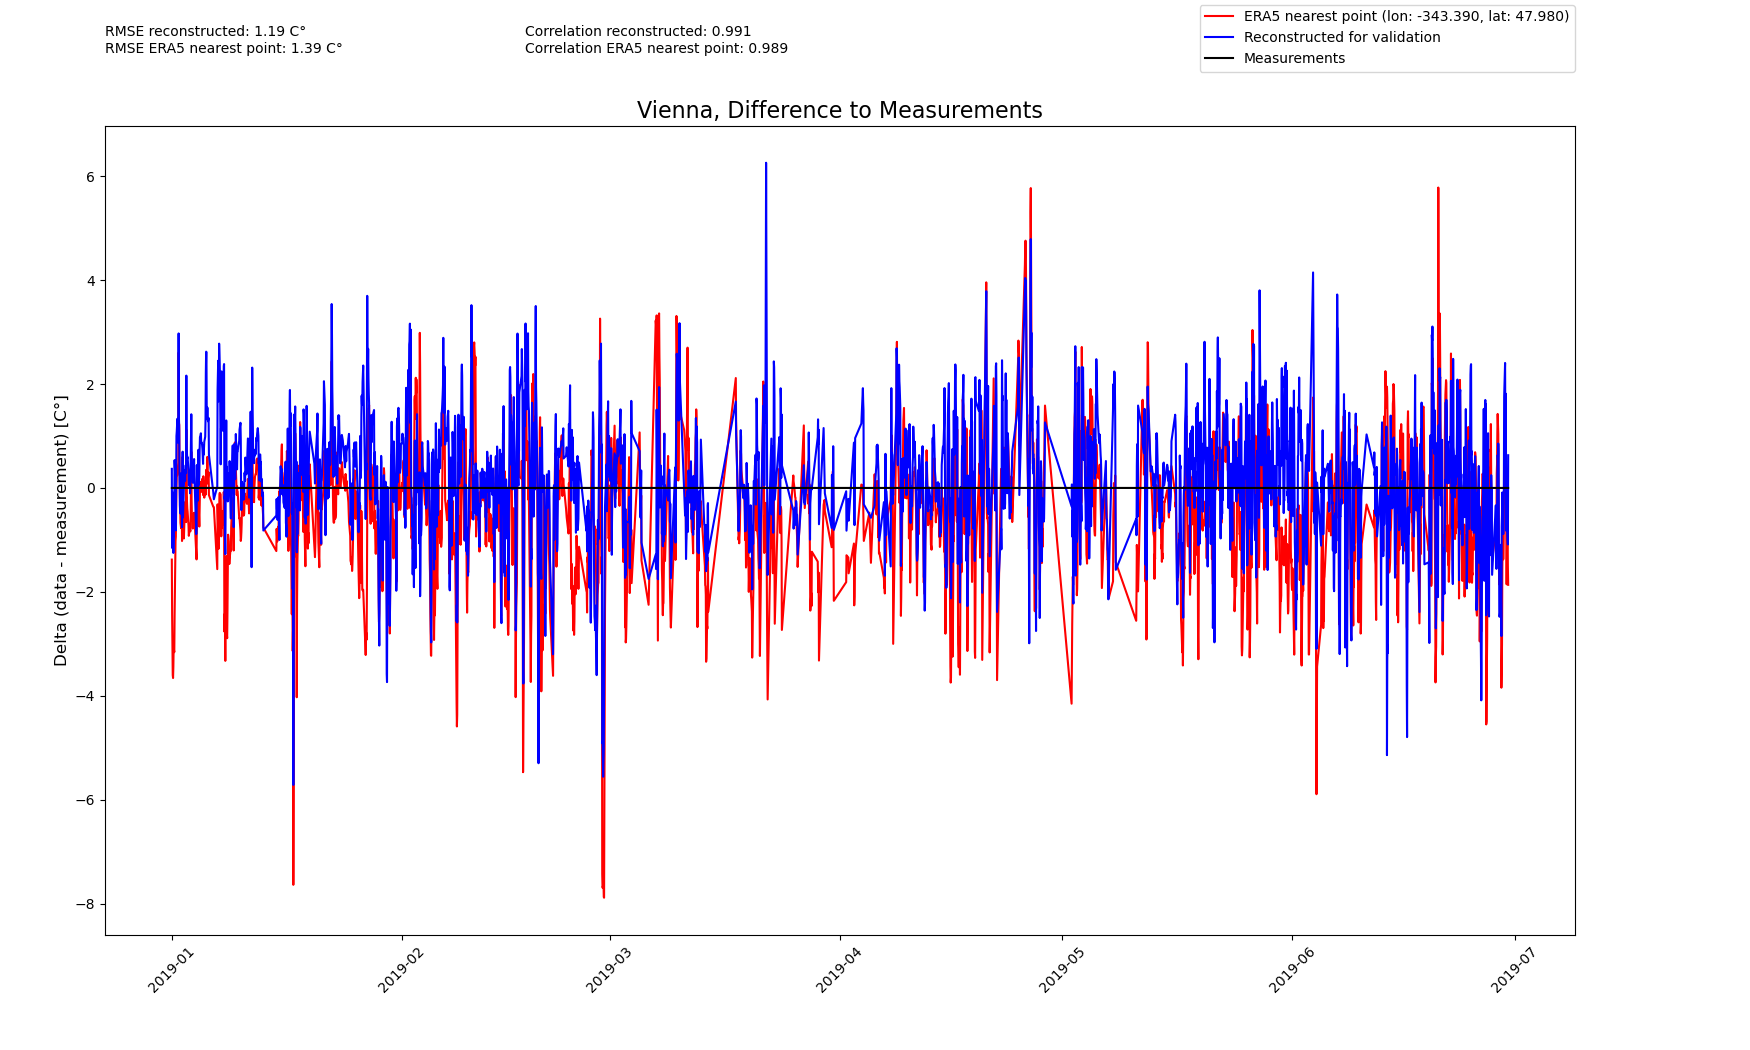
\includegraphics[width=1.00\textwidth]{resources/images/charts/vienna_eval_grib_final/Vienna, Difference to Measurements.png}
\caption{Difference between reconstructed and measured hourly temperature for Vienna-Station}
\end{figure}
% RMSE reconstructed: 1.19, RMSE ERA5: 1.39, Correlation reconstructed: 0.991, Correlation ERA5: 0.989

Similar to the Marshall-Station the plots for the Vienna-Station follow the same structure.
Again, a plot over the full validation period on an hourly basis, daily and monthly aggregated ones and the diurnal cycle as well as an extract of a week, are shown.
However, an important difference is that as the available data of the station in Vienna was so limited, we only included half a year in the validation data.
Also, to put the validation of the reconstruction in perspective, it needs to be considered that the RMSE and correlation coefficient, in relation to the ERA5 data in Vienna, are by far the best among the three stations.
1.19°C RMSE and 0.991 correlation coefficient for the reconstructed temperature compared to 1.39°C RMSE and 0.989 correlation coefficient for the ERA5 data at the nearest grid point.
The model was able to reduce the error slightly but not significantly.
This minor improvement can be attributed to the limited training data but also to the fact that the ERA5 data is already very similar to the station data.

\begin{figure}
\centering
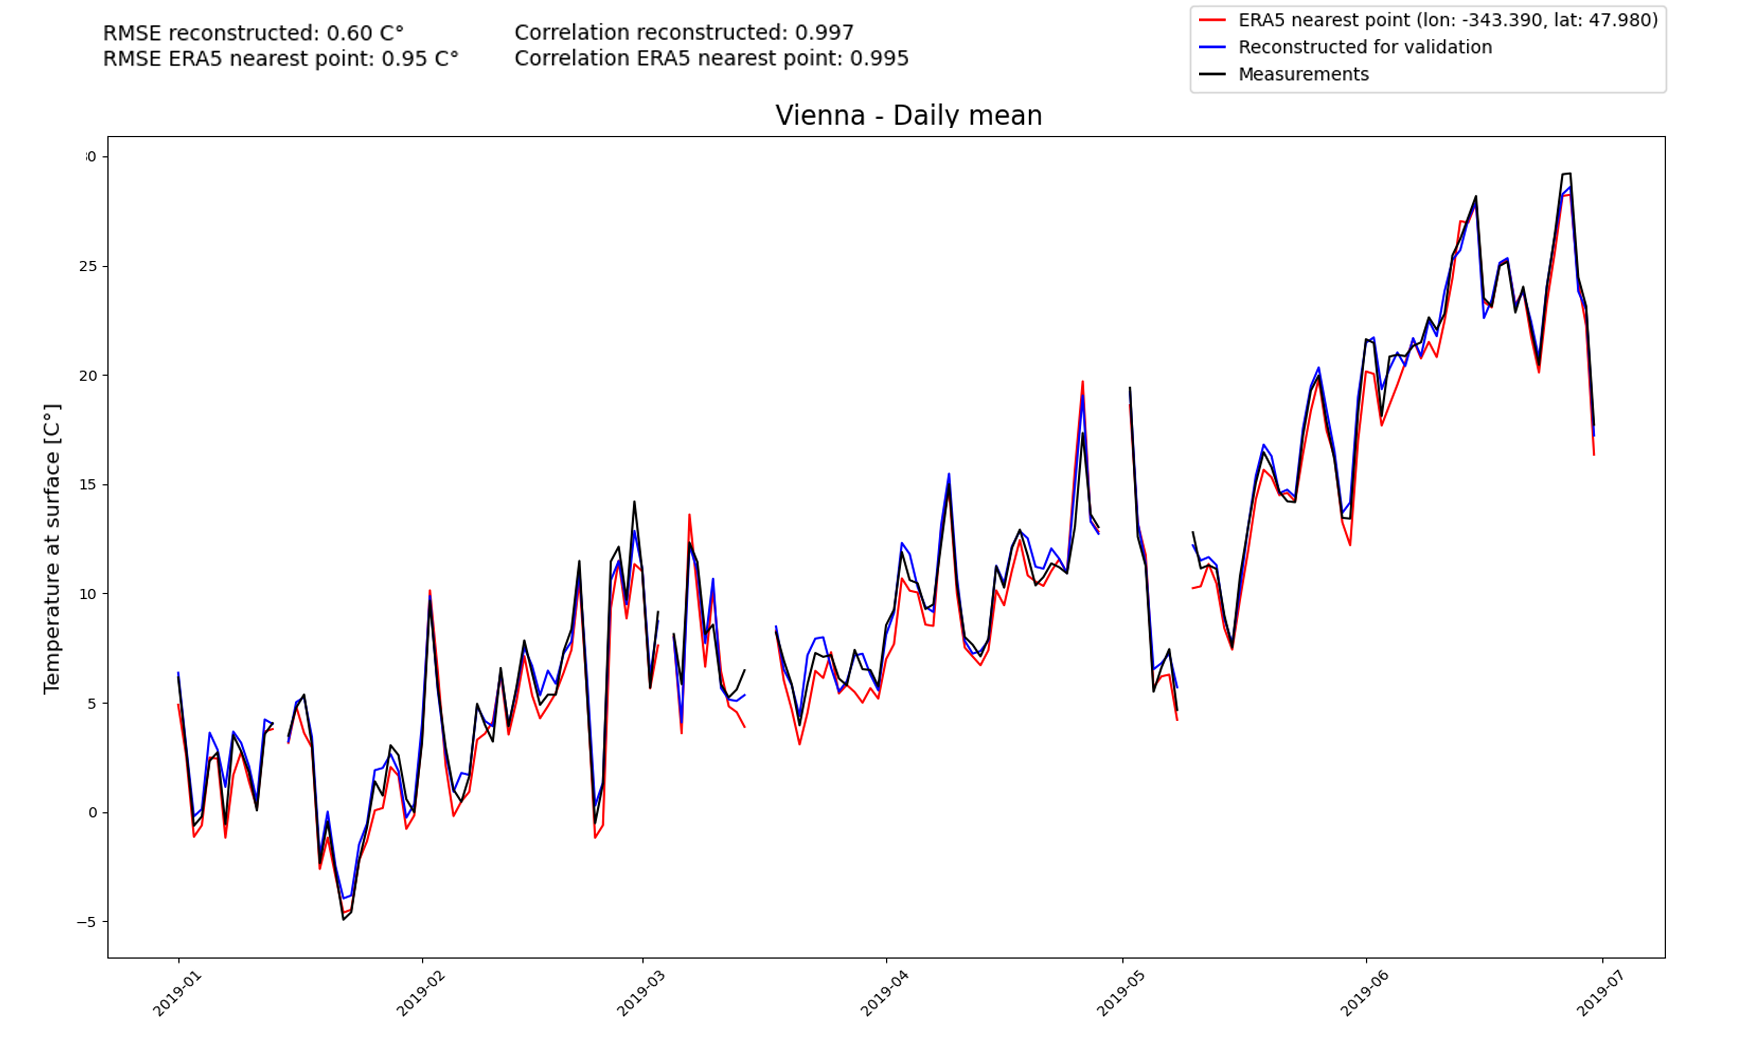
\includegraphics[width=1.00\textwidth]{resources/images/charts/vienna_eval_grib_final/Vienna - Daily mean.png}
\caption{Reconstructed temperature for Vienna-Station (Daily mean)}
\label{fig: vienna_daily}
\end{figure}
% RMSE reconstructed: 0.60, RMSE ERA5: 0.95, Correlation reconstructed: 0.997, Correlation ERA5: 0.995

Aggregating the hourly values to daily means, as shown in \autoref{fig: vienna_daily}, unsurprisingly improves the RMSE and correlation coefficient again, and allows for an absolute temperature scale on the y-axis.
It can be seen that as the temperature rises in Vienna from January to July until the station went offline.
It seems that the reconstruction is just marginally improving from its input data in terms of correlation coefficient.
However, the RMSE now at 0.60°C is by a relative measure significantly lower than the 0.95°C of the ERA5 data at the nearest grid point. 

\begin{figure}
\centering
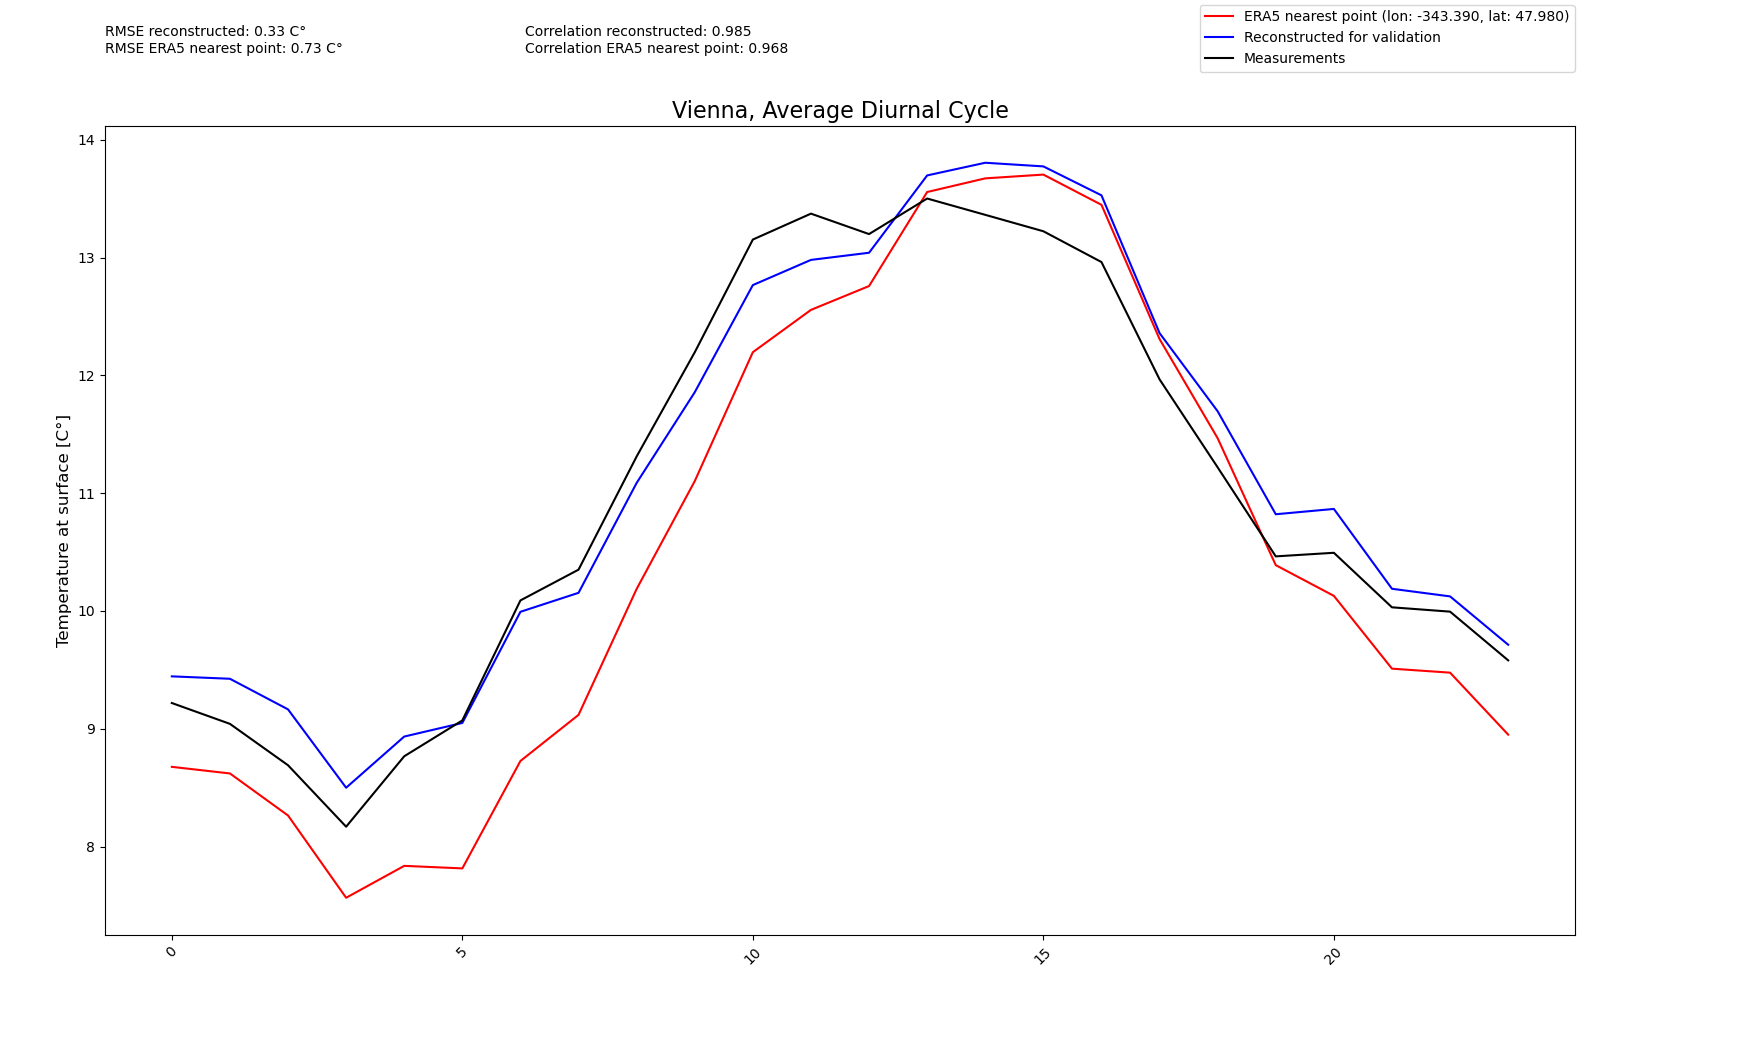
\includegraphics[width=1.00\textwidth]{resources/images/charts/vienna_eval_grib_final/Vienna, Average Diurnal Cycle.png}
\caption{Measured temperature for Vienna-Station (Average Diurnal Cycle)}
\label{fig: vienna_diurnal}
\end{figure}
% RMSE reconstructed 0.33, RMSE ERA5 0.73, Correlation reconstructed 0.985, Correlation ERA5 0.968

Figure \ref{fig: vienna_diurnal} of the diurnal cycle shows the best performance of the model in Vienna, with an RMSE of 0.33°C compared to 0.73°C for the ERA5 data.
The correlation coefficient of 0.968°C for the ERA5 data is the lowest among the different analyses for Vienna, which is due to the fact that there seems to be a time shift.
As the temperature rises at the beginning of the day, the station temperature seems to be approximately one hour ahead of the ERA5 temperature.
The model was able to correct this time shift, leading to this excellent RMSE and correlation coefficient of 0.985.

\begin{figure}
\centering
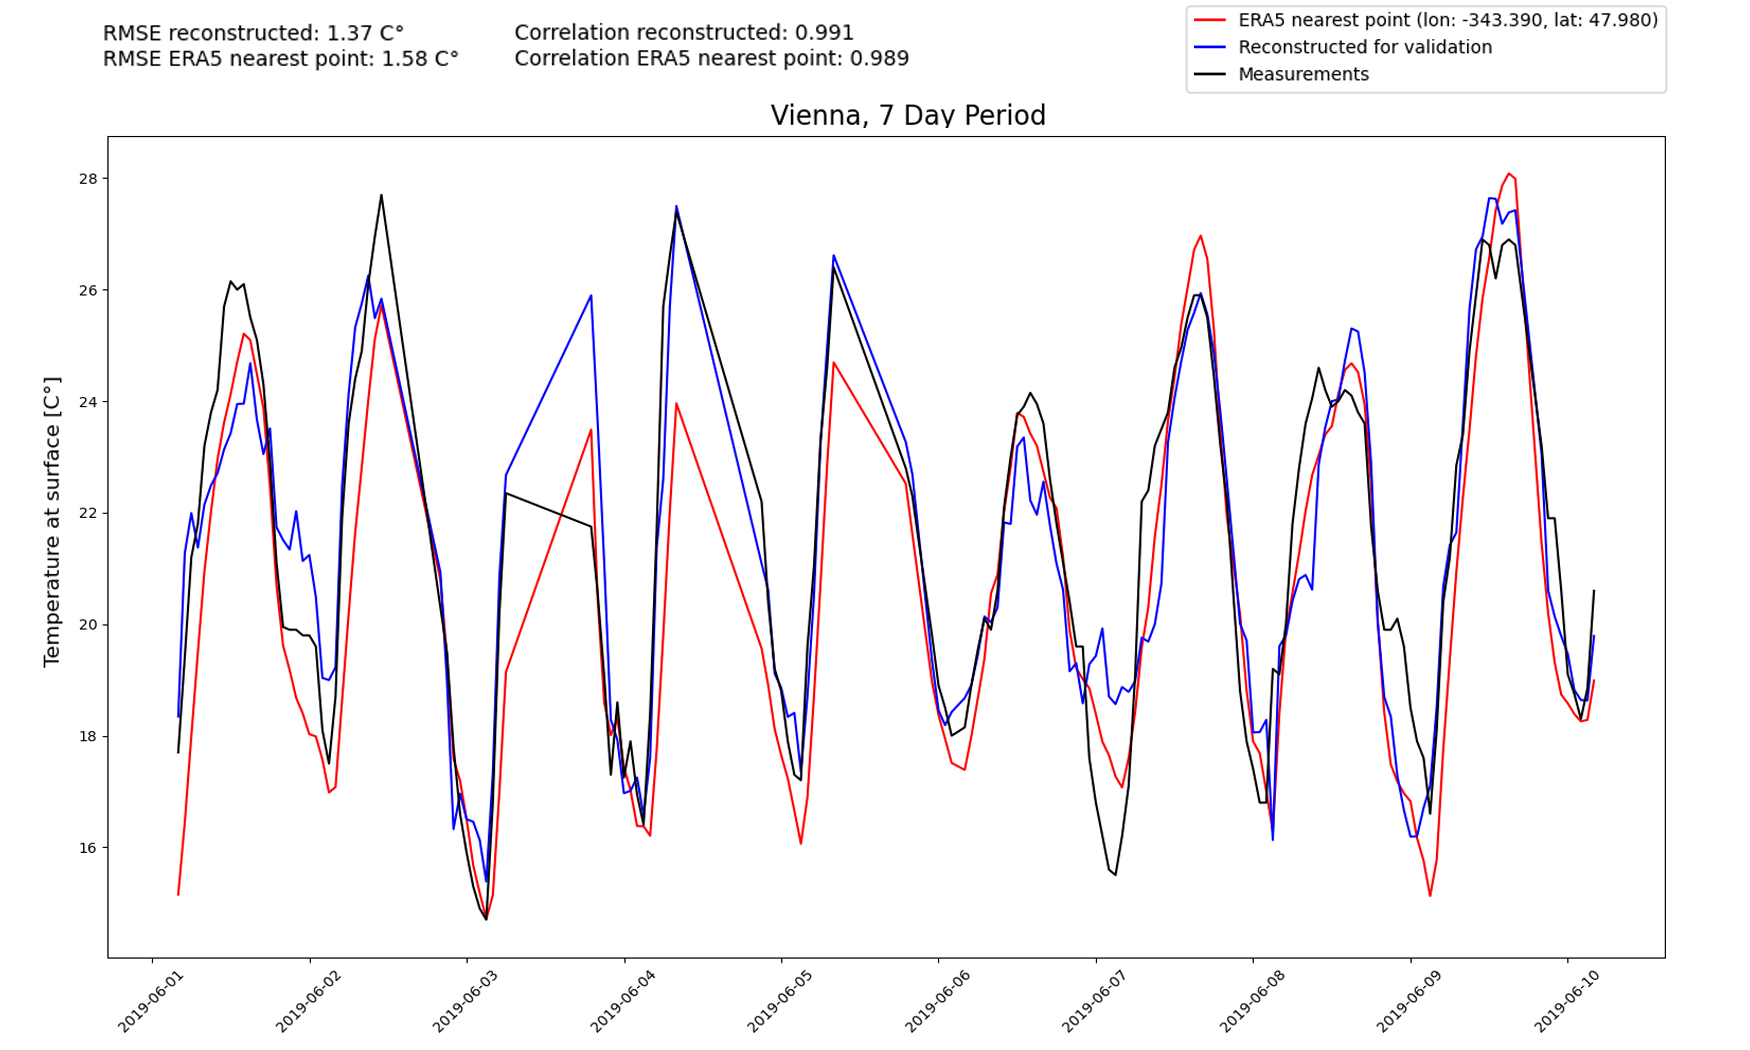
\includegraphics[width=1.00\textwidth]{resources/images/charts/vienna_eval_grib_final/Vienna, 7 Day Period_1_2_3.png}
\caption{Reconstructed temperature vs. measured hourly temperature for Vienna-Station (7 Day Period)}
\label{fig: vienna_7day}
\end{figure}

\begin{figure}
\centering
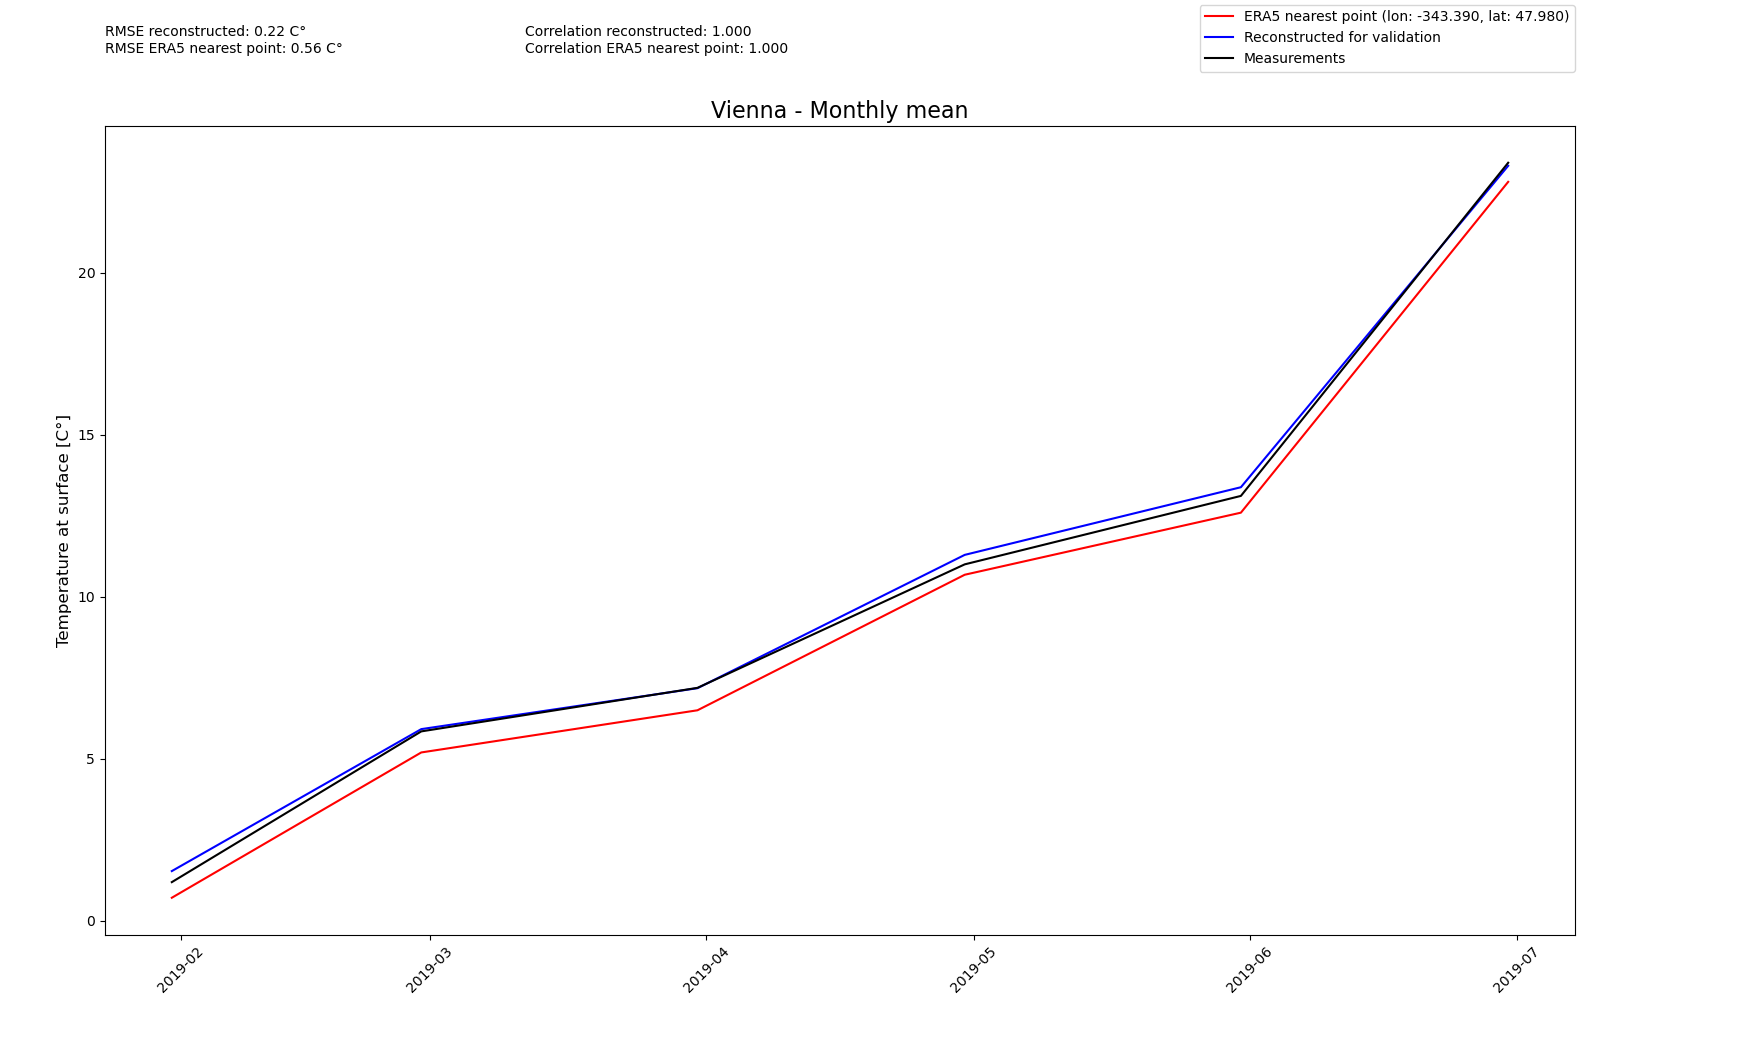
\includegraphics[width=1.00\textwidth]{resources/images/charts/vienna_eval_grib_final/Vienna - Monthly mean.png}
\caption{Reconstructed temperature vs. measured temperature for Vienna-Station (Monthly mean)}
\label{fig: vienna_monthly}
\end{figure}
% RMSE reconstructed 0.22, RMSE ERA5 0.56, Correlation reconstructed 1.000, Correlation ERA5 1.000

When aggregating to a monthly mean, it becomes further visible how close the ERA5 and reconstructed temperature are to the measurements. The correlation coefficients are both 1.000, indicating a perfect correlation.
The only issue visible is that ERA5 has a slightly low bias, which the model minimally overcorrects.

\subsubsection*{Barbados-Station}

\begin{figure}
    \centering
    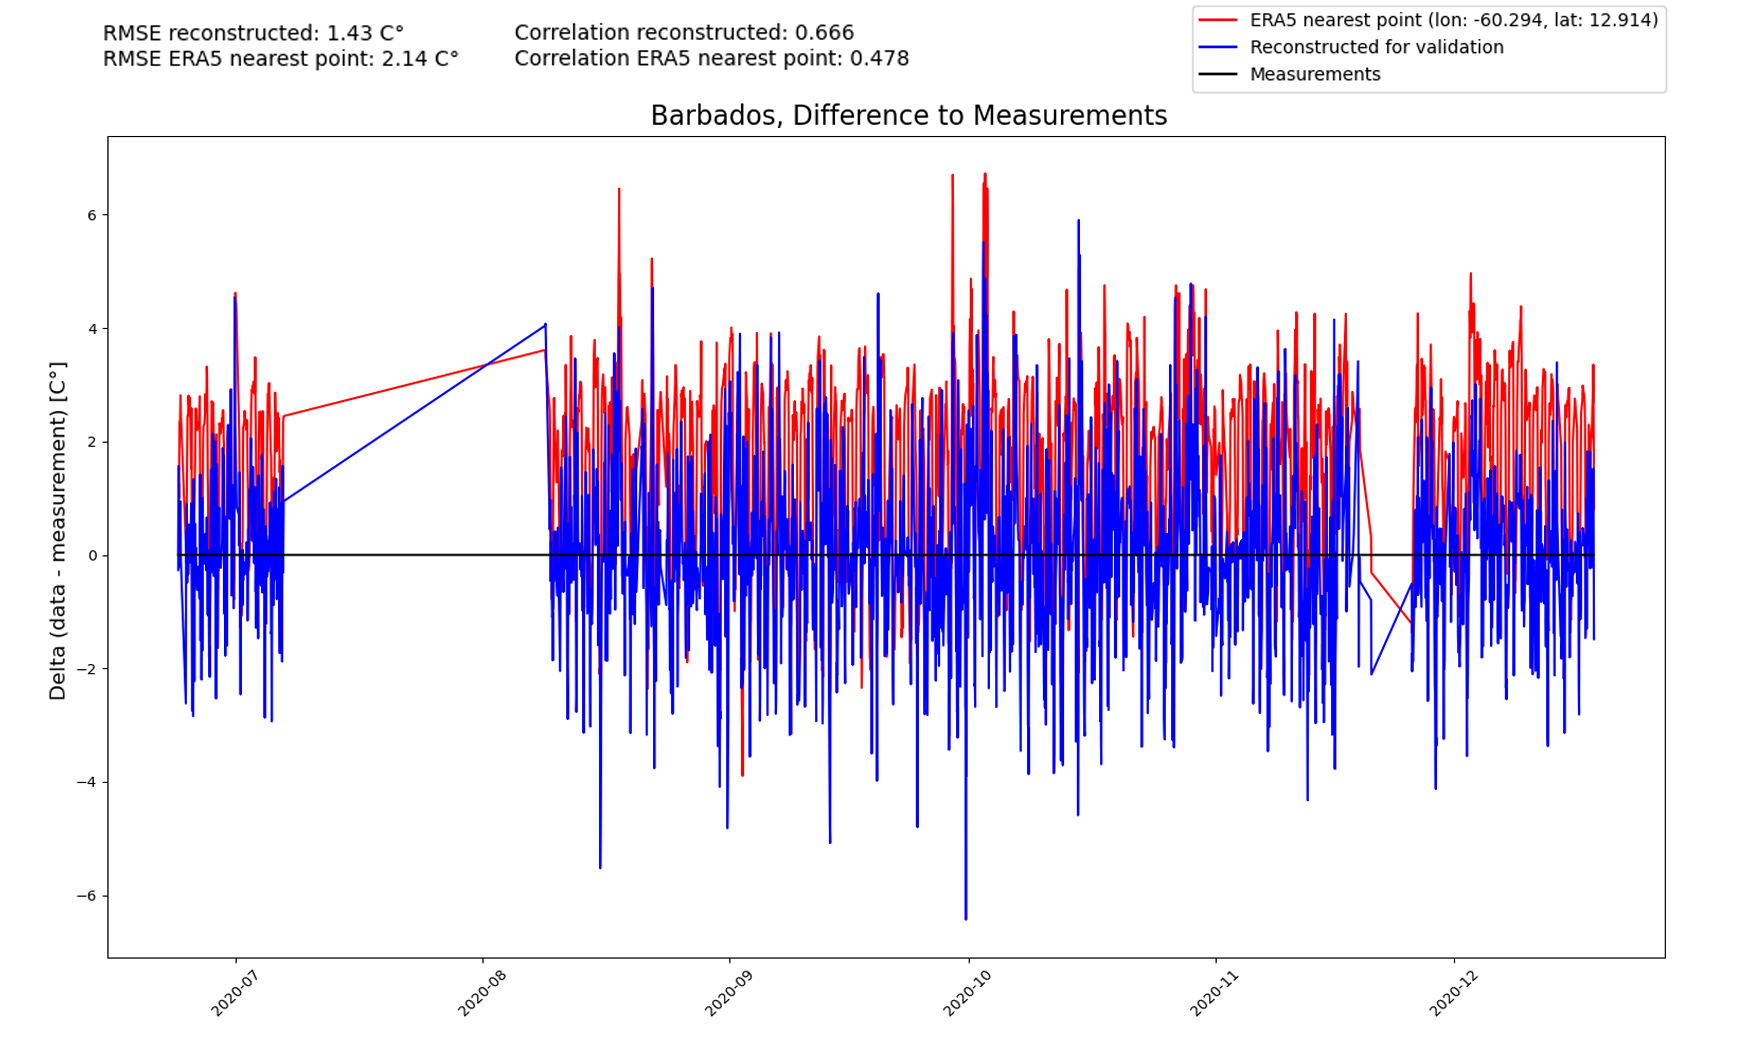
\includegraphics[width=1.00\textwidth]{resources/images/charts/barbados_eval_grib_final/Barbados, Difference to Measurements.png}
    \caption{Difference between reconstructed and measured hourly temperature for Barbados-Station}
\end{figure}
% RMSE reconstructed: 1.43, RMSE ERA5: 2.14, Correlation reconstructed: 0.666, Correlation ERA5: 0.478
% super low correlation for era5, improved but compared to other stations still low
% big gap  visible again of 1month+ in the beginning because missing data

\begin{figure}
    \centering
    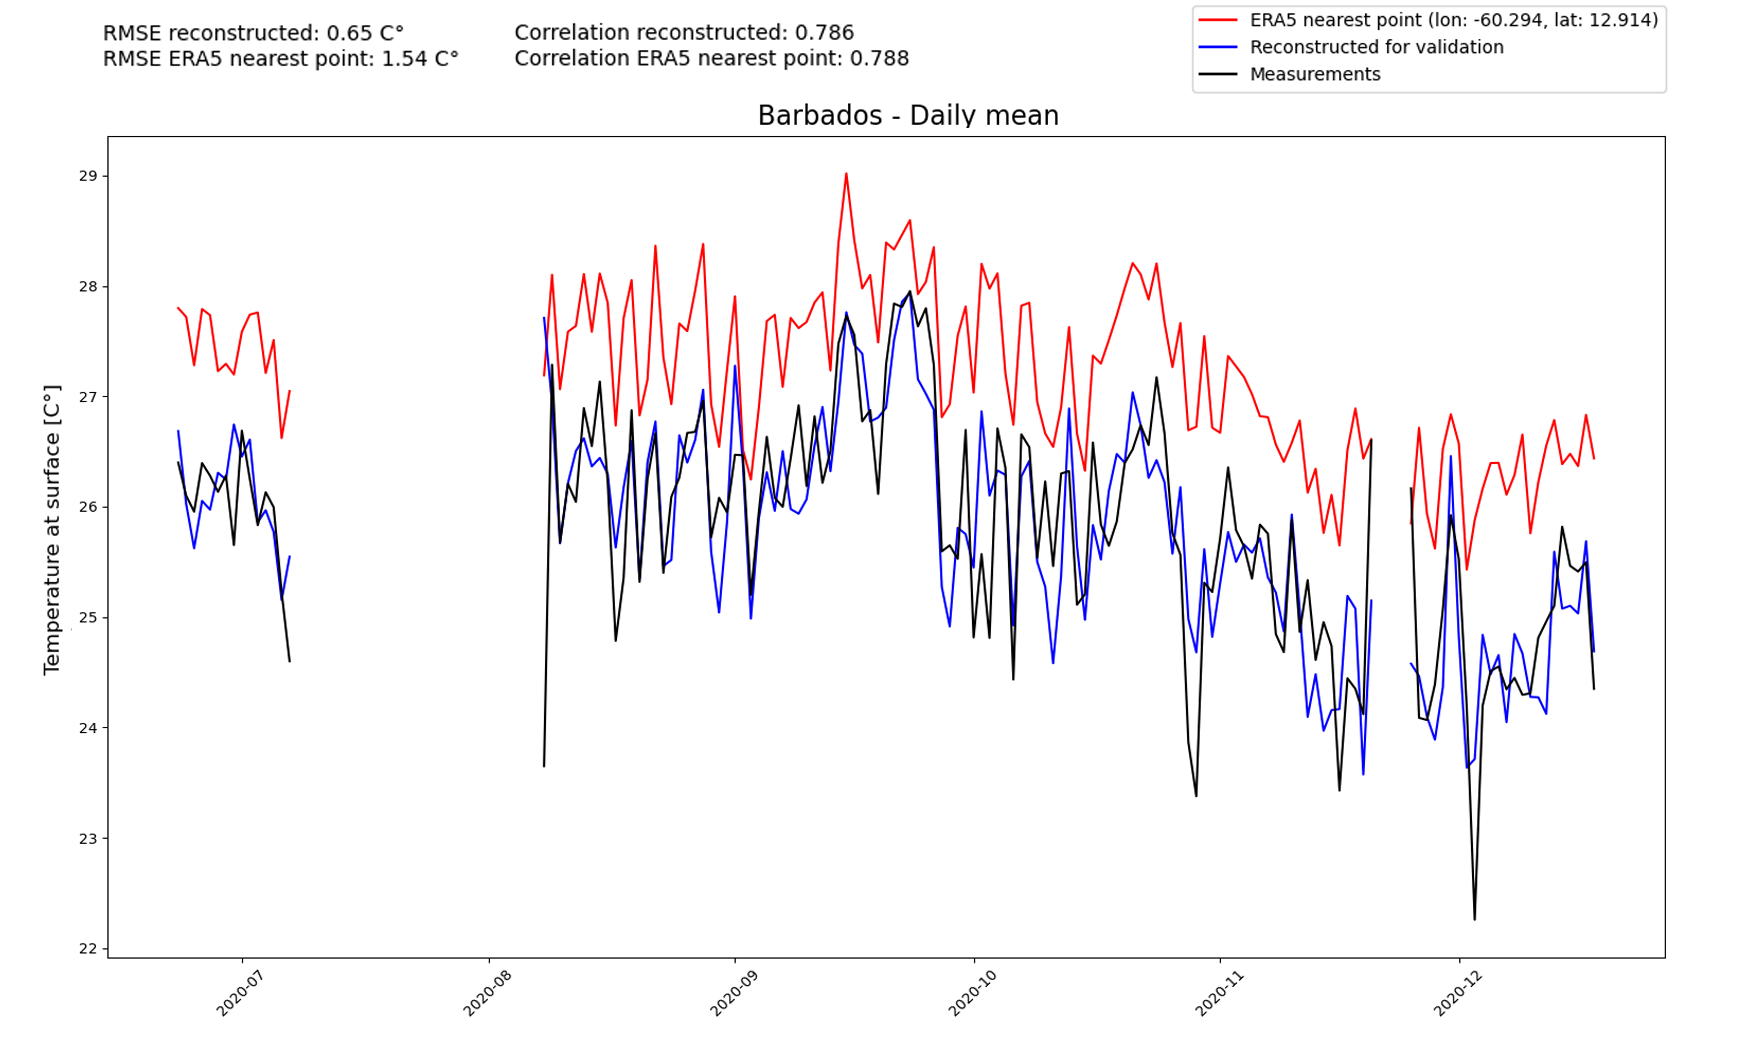
\includegraphics[width=1.00\textwidth]{resources/images/charts/barbados_eval_grib_final/Barbados - Daily mean.png}
    \caption{Reconstructed temperature for Barbados-Station (Daily mean)}
\end{figure}
% RMSE reconstructed: 0.65, RMSE ERA5: 1.54, Correlation reconstructed: 0.786, Correlation ERA5: 0.788
% on daily basis correlation fairly high again, as the biggest difference in Barbados comes through the diurnal cycle

\begin{figure}
    \centering
    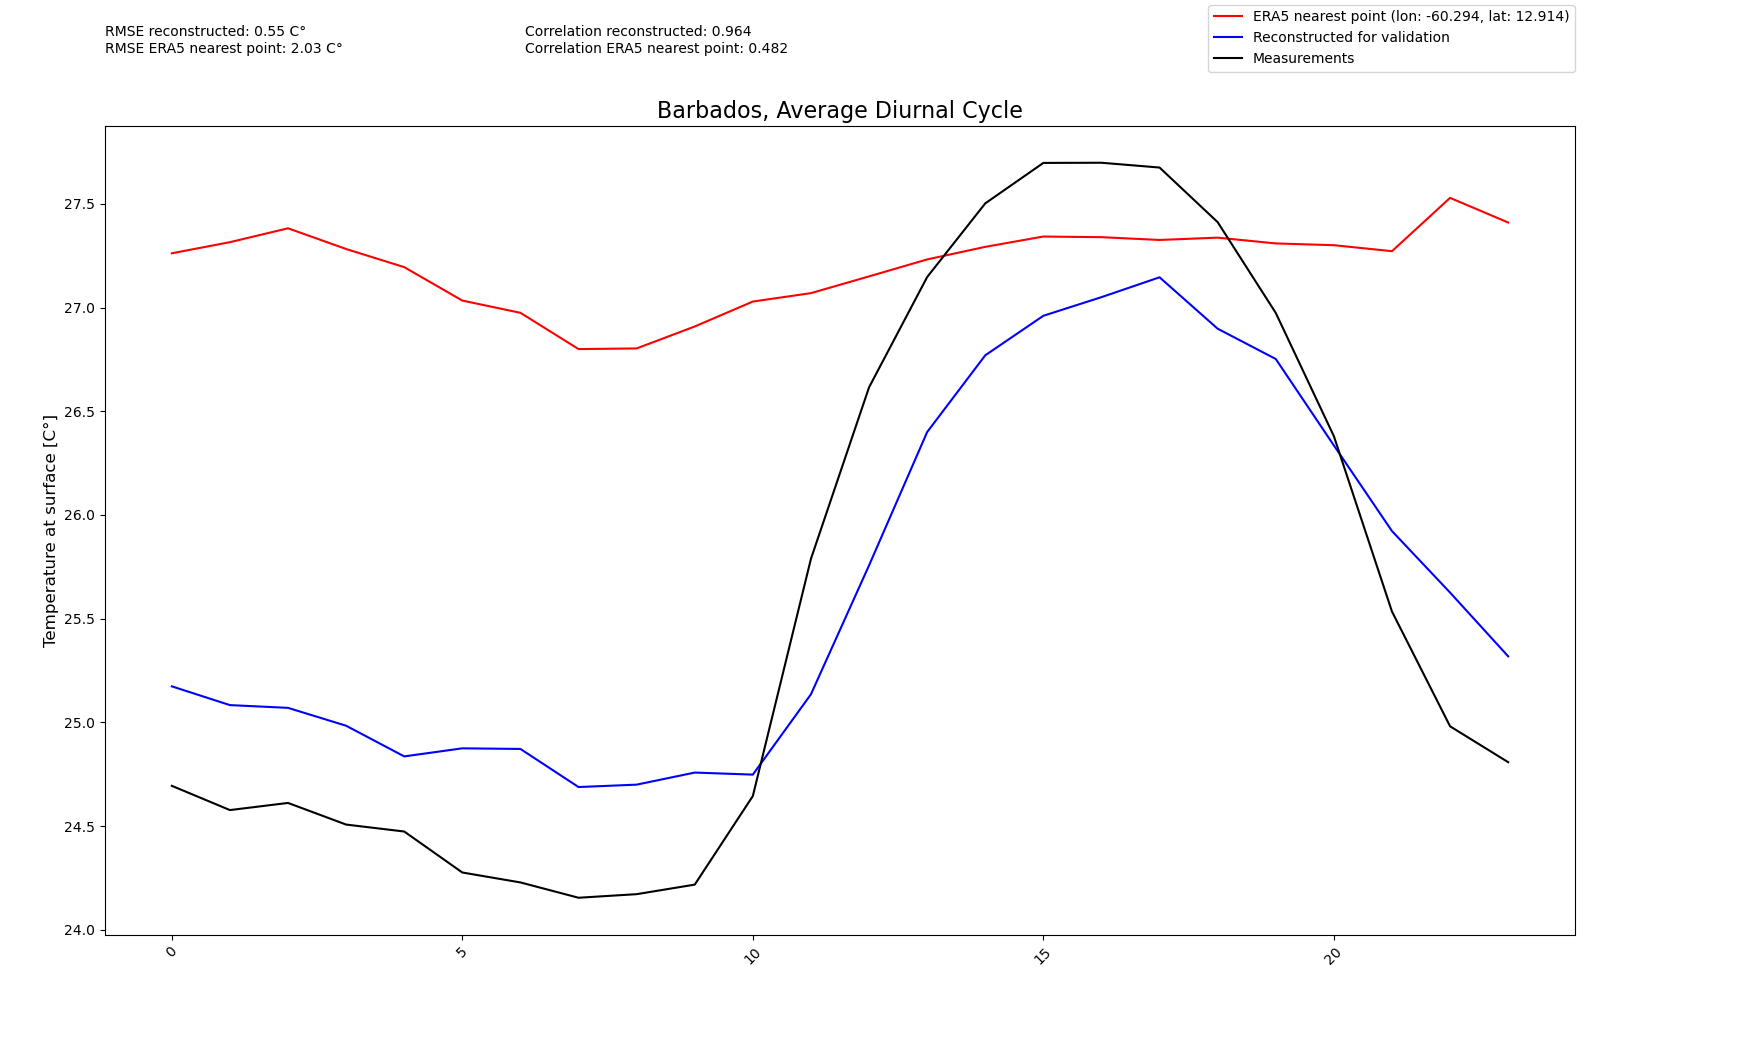
\includegraphics[width=1.00\textwidth]{resources/images/charts/barbados_eval_grib_final/Barbados, Average Diurnal Cycle.png}
    \caption{Measured temperature for Barbados-Station (Average Diurnal Cycle)}
\end{figure}
% RMSE reconstructed 0.55, RMSE ERA5 2.03, Correlation reconstructed 0.964, Correlation ERA5 0.482
% super good effort here in the reconstruction, the diurnal cycle in era5 which was the input data is basically flat, hence has a low correlation, but the model was able to reconstruct the diurnal cycle of the station to a point where the correlation is really high again, however the amplitude of the diurnal cycle is not as high as in the measurements, corr coeff still high as it's just linear-relationship thingy


\begin{figure}
    \centering
    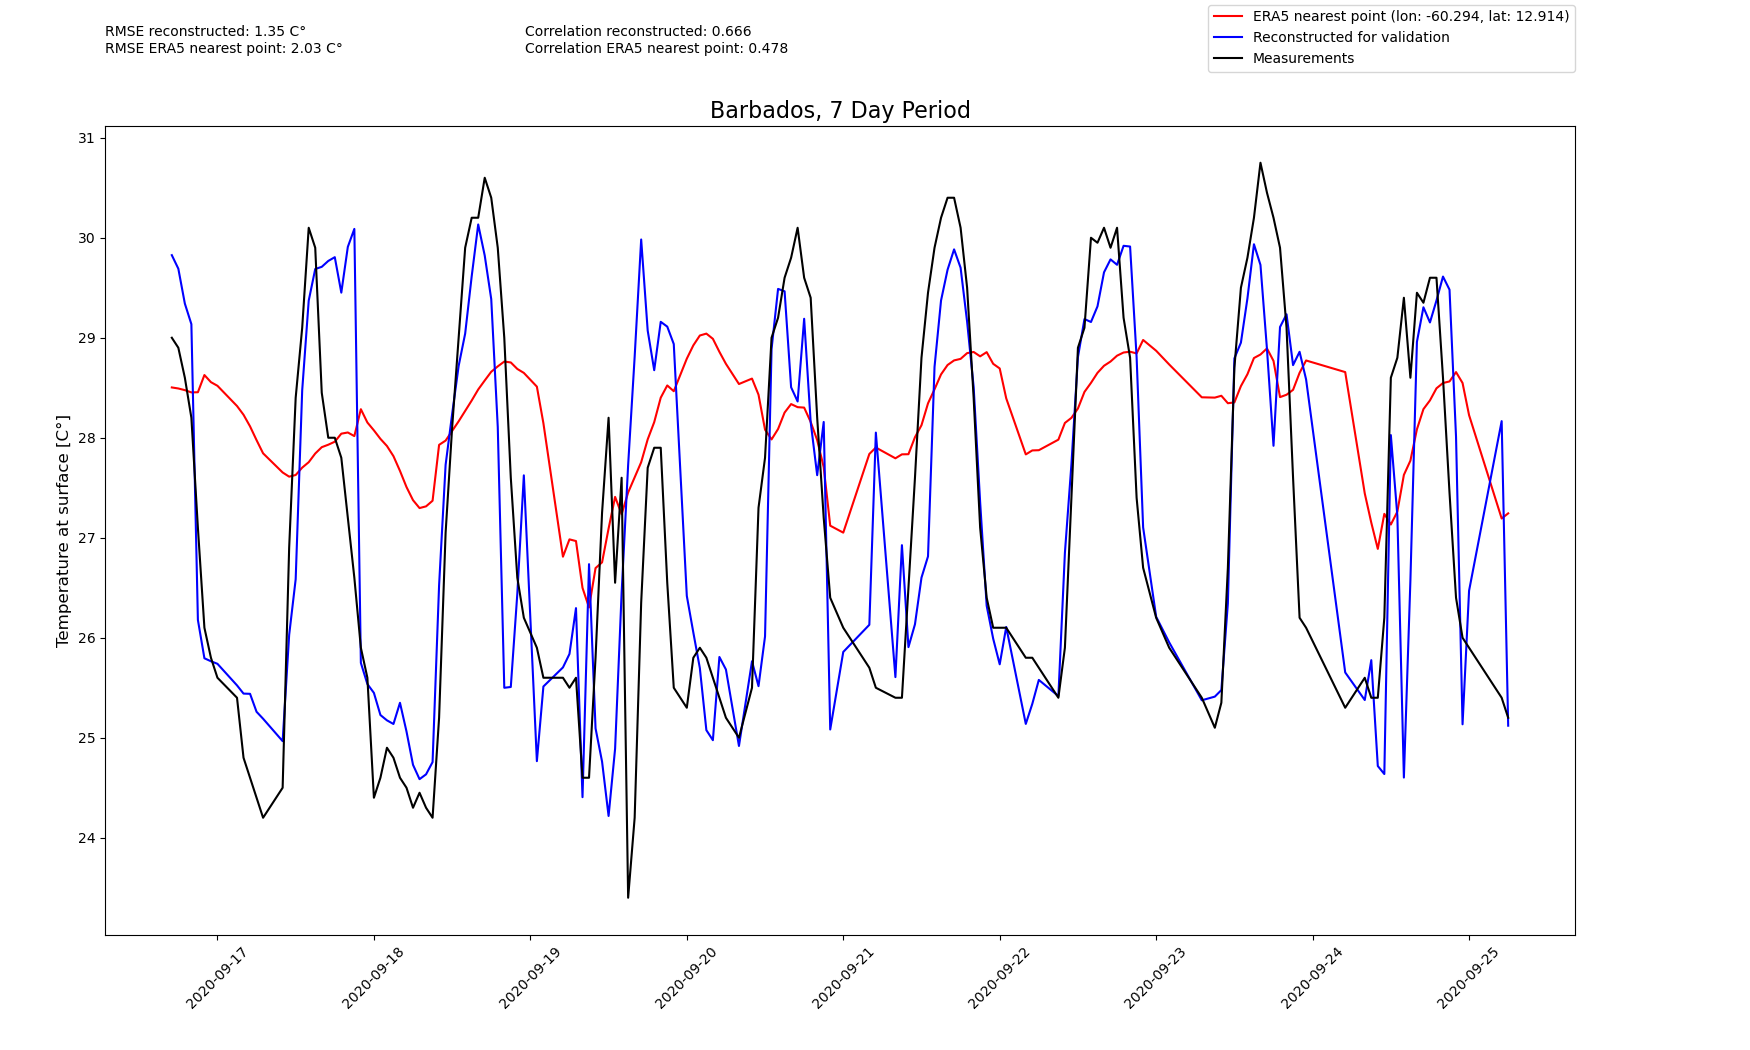
\includegraphics[width=1.00\textwidth]{resources/images/charts/barbados_eval_grib_final/Barbados, 7 Day Period_1_2.png}
    \caption{Reconstructed temperature vs measured hourly temperature for Barbados-Station (7 Day Period)}
\end{figure}

\begin{figure}
    \centering
    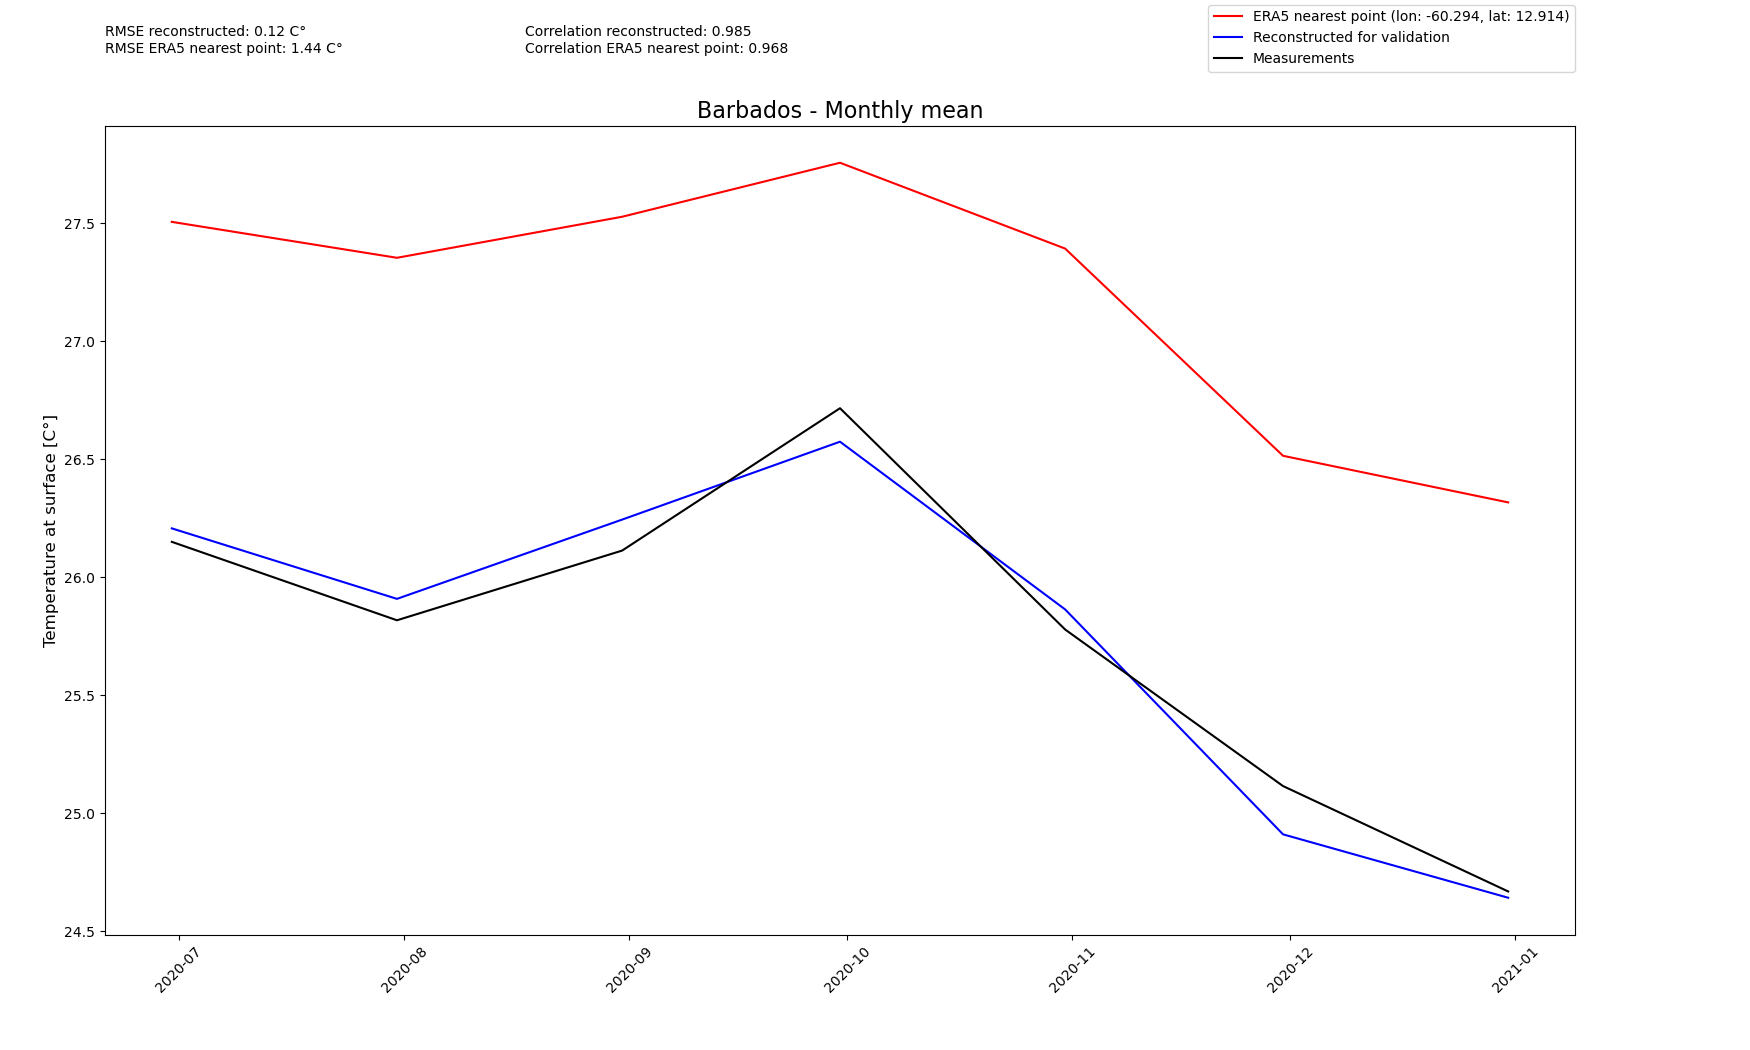
\includegraphics[width=1.00\textwidth]{resources/images/charts/barbados_eval_grib_final/Barbados - Monthly mean.png}
    \caption{Reconstructed temperature vs measured temperature for Barbados-Station (Monthly mean)}
\end{figure}
% RMSE reconstructed 0.12, RMSE ERA5 1.44, Correlation reconstructed 0.985, Correlation ERA5 0.968
% rmse seems low but it needs to be considered that the diurnal cycle is not as pronounced in the measurements as in the other stations, hence the rmse is lower, compared to corr coeff on monthly basis of matshall and vienna, barbados is difficult...

\newpage
% Portable Software -> new repository
\section{Software Implementation}
\label{sec:implementation}

\subsection{Introduction}

Given that the machine learning part of the software is modulized as "Climate Reconstruction AI" (CRAI), such that the actual setup of the neural net, training and evaluation afterwards is outsourced. Thus the process for a single specific dataset of one station could be written pretty straightforward with a NetCDF file of the station data ahead, if there is sufficient access to ERA5 Data. A Jupyter notebook could be sufficient as a way to start. However once dealing with different stations, different ERA5 files need to be stored, and the files that have been prepared for submission into CRAI need to have some kind of management and the "training-args" for CRAI need to be adapted each time. Thus it appears natural to implement a set of functions and structure the process through an object-oriented approach. This allows control of different but similar pipelines with a few lines of code, either through a script, initiated by an API or in a Jupyter notebook.
This chapter is about laying the foundation through the implementation of the different steps of the pipeline as classes and functions, while in chapter \autoref{sec:process_orchestration} the next abstraction level of the software into classes that handle the execution of the different steps and the interaction with the user through an API and a web interface is described.
The following subsections highlight the key steps of the pipeline and how their functionality evolves. It does not cover the detailed embedding of the methods in their classes, nor is explicitly mentioned where temporary folders would be created to establish a philosophy where each step of the pipeline is implemented independently and can be connected in a higher-level class. The methods are not necessarily designed to be used in any possible order and more in the sense of the desired pipelines, but the modularity allows for a better understanding and cleaner code, which is essential when developing another layer of abstraction later.

\begin{figure}
    \centering
    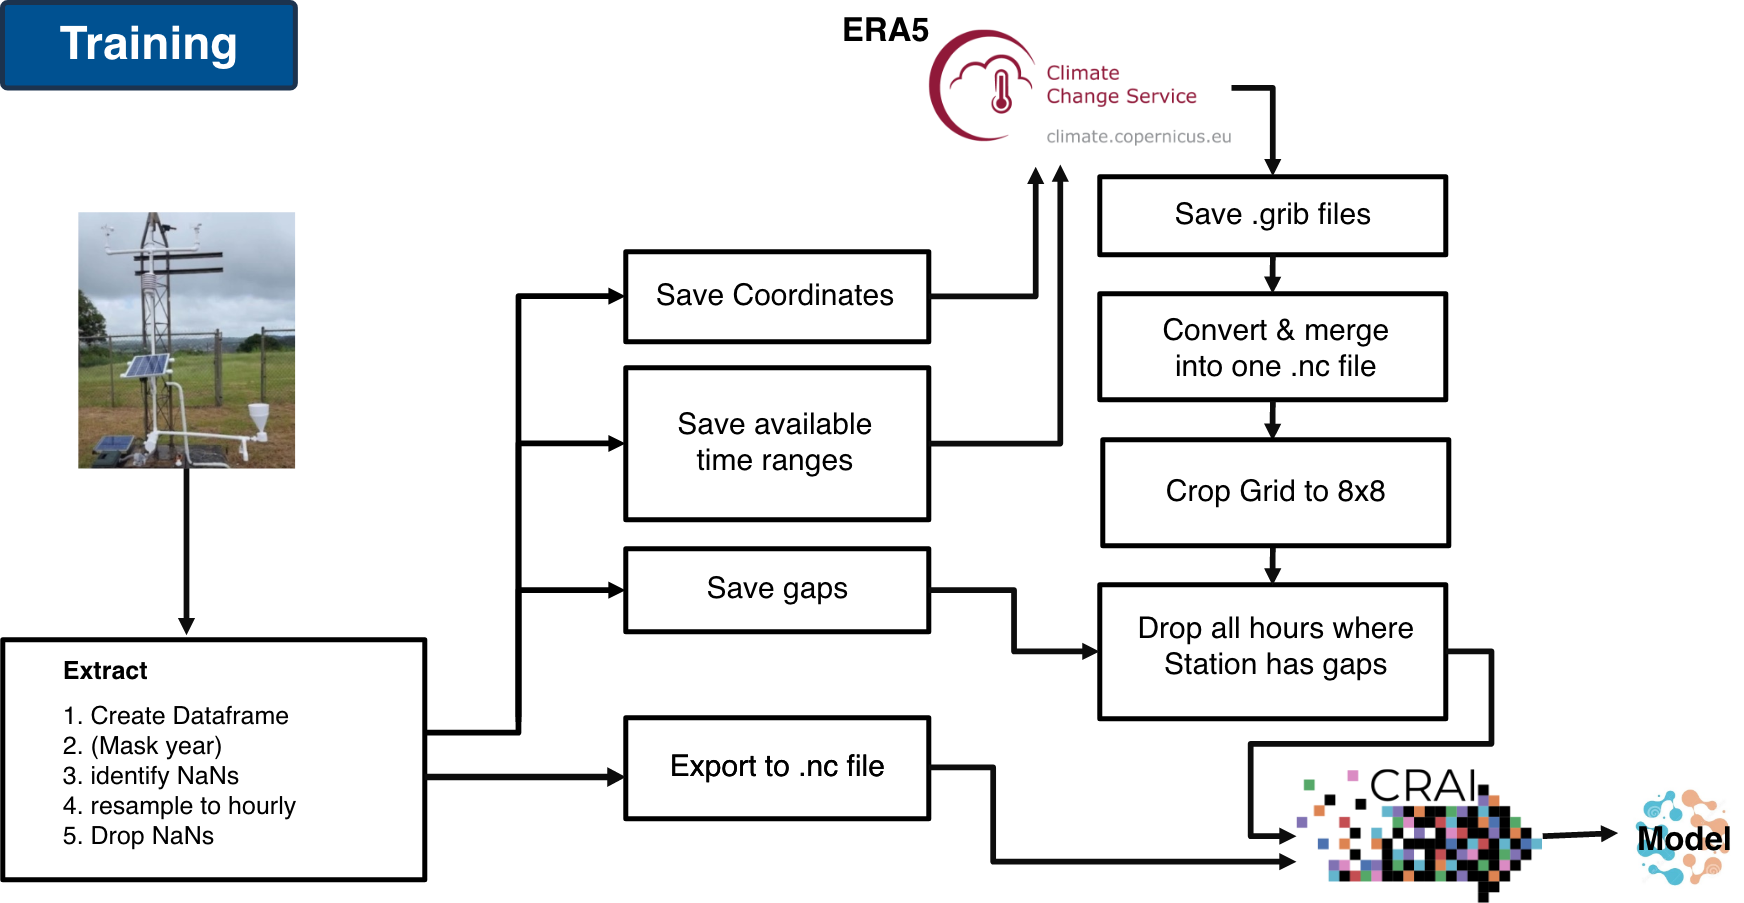
\includegraphics[width=450pt]{resources/images/training_pipeline.png}
    \caption{Pipeline to train a model}
    \label{fig:training_pipeline}
\end{figure}

\begin{figure}
    \centering
    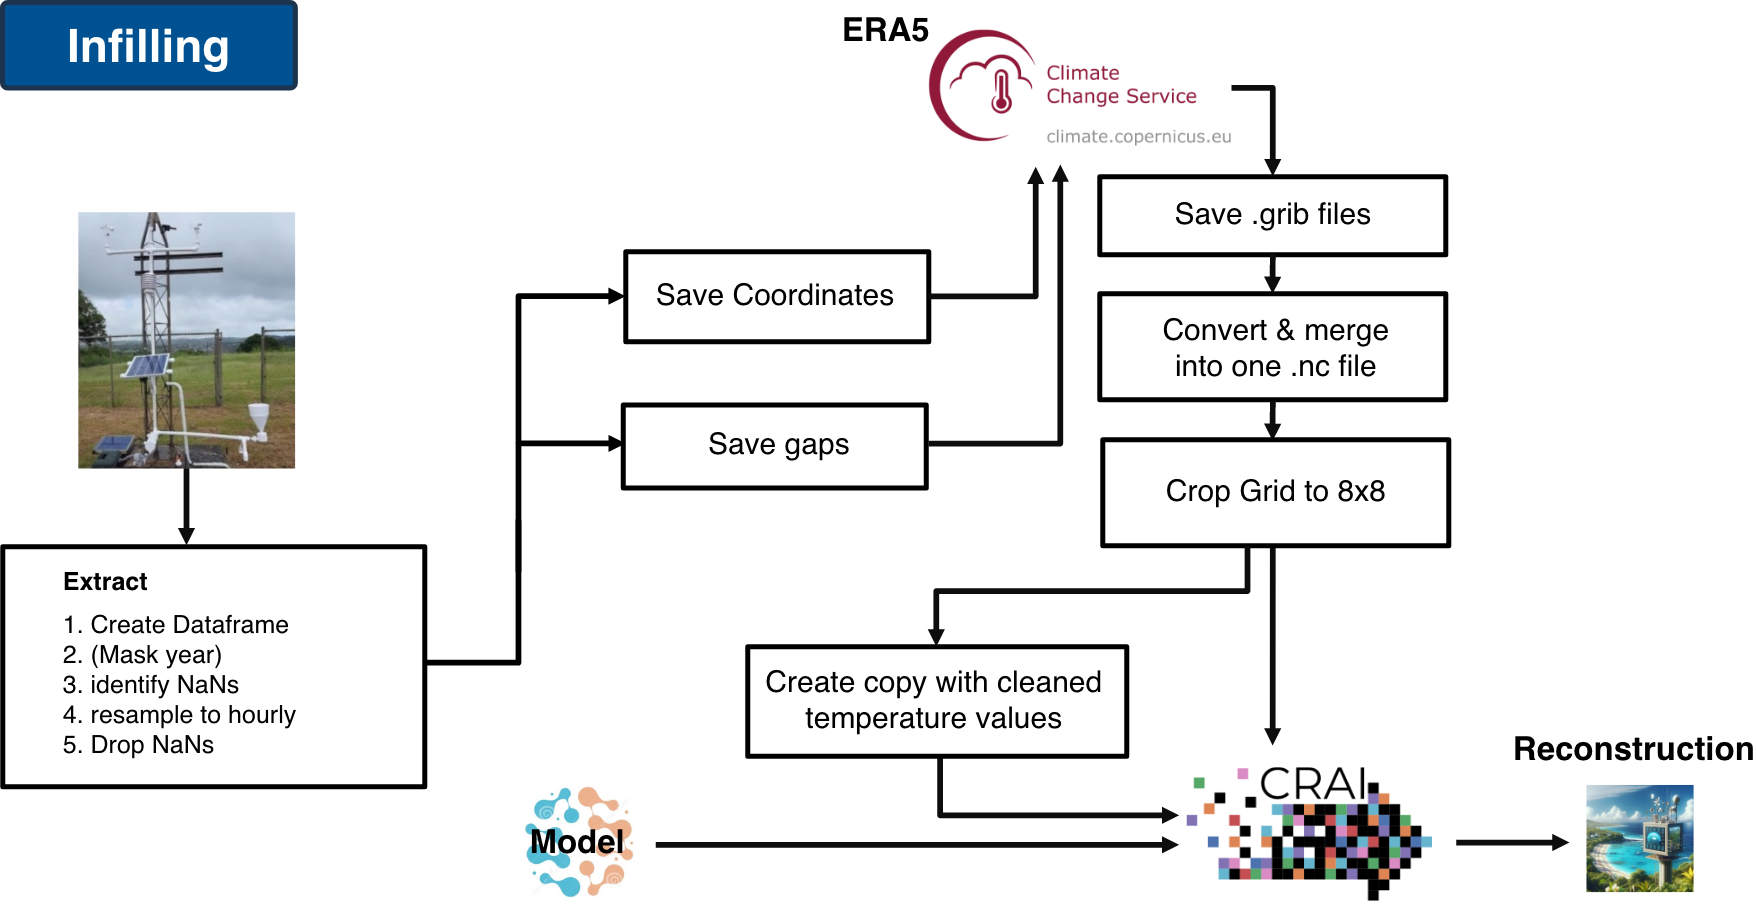
\includegraphics[width=450pt]{resources/images/infilling_pipeline.png}
    \caption{Pipeline to reconstruct weather data using a model}
    \label{fig:infilling_pipeline}
\end{figure}

\subsection{Stationdata Submission \& Conversion}

The station data for the 3D printed weather stations provided by NCAR comes in delimited text files, with one file per day and a text-based metadata file holding information like the station name, the latitude and longitude and the elevation.
The data files (.dat files) hold per sensor one column and per minute one row.

A class "DatToNcConverter" is implemented with the following main use cases:
First to take in a directory with the .dat files and the metadata file and parse it. Second to process the data including dropping missing values as well as resampling to an hourly frequency, and converting from Celcius to Kelvin to match ERA5. This is easiest in a pandas dataframe. Third to convert the data to a NetCDF file, which is the format that is used by the ERA5 data and the CRAI module. The NetCDF file is structured in a way that the data is stored in a 3D array with the dimensions time, latitude and longitude. The metadata is stored as global attributes in the NetCDF file. Fourth to convert some dataframe back to a .dat file after the reconstruction of measurements to match the original format when infilling. Of these use cases the one resampling to hourly frequency is the most complex, or at least could include many design decisions. Missing values are marked with "-999.99", so in the first step, these values can be marked as NaN. However, the data quality is by default not controlled and there could be values that should be marked as missing but are not. Thus the NCAR consulted to mark "0.00" °C as NaN. For stations like Barbados this wouldn't be a realistic value anyway, but even for regions where 0°C degrees are reached often, it's unlikely to measure exactly "0.00", meaning the amount of correct data lost through marking "0.00" as NaN is still limited. Also by agreement with the NCAR everything above or under +/- 45°C is marked as NaN. Additionally to compensate for peaks in the data aggregating the minutes using a median instead of a mean can be a good idea, numpy.median() would return NaN if any value is NaN and numpy.nanmedian() would ignore NaNs. It would be best to have a custom aggregate function using numpy.nanmedian() but assuring prior to that that there are sufficient non-NaN values.

For the usecase of converting the data back to a .dat file, the dataframe is stored directly in the converter object as original dataframe after detecting NaNs and resampling to hourly values, before any transformation of units (Celcius to Kelvin) or renaming of columns takes place and before NaNs are dropped. Fundamentally inbetween the first and last measurements rows for all minutes exist, even if measurements are missing. However if the station had severe issues it's possible that between first and last record there are even rows or files missing. To assure that the original dataframe will have rows for all hours, a handy method provided by the python pandas module is used:

\begin{lstlisting}
    self.original_df = self.original_df.reindex(
        pd.date_range(start = self.dataframe.index.min(), end = self.dataframe.index.max(), freq = "h"))
\end{lstlisting}

A class "Station" is implemented to hold the metadata and the pandas dataframe of the station data. It holds the converter itself, to minimize lines of code in the main script. The class is mainly used to manage the access to the different files and data, before and after the conversion. And secondly to detect the gaps in the data, for infilling simply in the form of listing the hours where data is missing. And for training use cases additionally in form of listing the months where at least some data is available which is most convenient for the API applicance to get ERA5 data for the station.


\begin{lstlisting}[caption=Gap Detection in Station Class, label=lst:find_gaps]
def find_gaps(self) -> None:
available_hour_steps = self.df.index
all_hour_steps = self.converter.original_df.index
# find all hours between the first and last hour that are missing
missing_hours = all_hour_steps.difference(available_hour_steps)
return missing_hours.tolist()
\end{lstlisting}

\begin{lstlisting}[caption=Detection of available ranges in Station Class, label=lst:available_ranges]
def get_all_months_in_df(self) -> None:
# return all (year, month) tuples in the dataframe
periods = self.df.index.to_period('M').unique().tolist()
month_dict = {}
for period in periods:
    if period.year not in month_dict:
        month_dict[period.year] = []
    month_dict[period.year].append(period.month)
return month_dict
\end{lstlisting}

\subsection{Copernicus Climate Data Store - CDS API}
\label{sec:cds_api}

The Copernicus Climate Data Store (CDS) is a service by the European Centre for Medium-Range Weather Forecasts (ECMWF). The CDS API provides opensource access to the ERA5 data, allowing users to download the data for a specific location and time period. After creating an account online an API Key can be obtained for free and with the python module 'cdsapi' data can be downloaded then easily in .grib format. 

\begin{lstlisting}[caption=Download Hook for ERA5 Data, label=lst:download_hook]
import cdsapi

class Era5DownloadHook:
    
    def __init__(self, lat, lon):
        self.cds = cdsapi.Client(
            url="https://cds.climate.copernicus.eu/api/v2",
            key=f"{os.getenv('UID')}:{os.getenv('API_KEY')}"
        )
        self.lon, self.lat = lon, lat

    def _download(cds, date_info, save_to_file_path):
        cds.retrieve(
        'reanalysis-era5-single-levels',
        {
            "product_type": "reanalysis",
            "format": "grib",
            "variable": "2m_temperature",
            "area": [
                self.lat + 1, # limit north
                self.lon - 1 % 360, # limit west
                self.lat - 1, # limit south
                self.lon + 1 % 360, # limit east
            ],
            "year": date_info.get("years"),
            "month": [f"{month:02d}" for month in date_info.get("months")],
            "day": [f"{day:02d}" for day in date_info.get("days")],
            "time": [f"{hour:02d}:00" for hour in date_info.get("hours")]

        }, save_to_file_path)



\end{lstlisting}

As seen in the code snippet, the request needs to include besides basic informations such as variable / format / model, the regional selection and the selection in the time dimension.
to download a few hours in a day the following can be used. When building requests that download a month or a full year, it becomes obvious why the \autoref{lst:available_ranges} is so useful.

\begin{lstlisting}[caption=Download Hours in Same Day in Download Hook Class, label=lst:download_hours_in_same_day]
    def download_hours_in_same_day(self, year, month, day, hours, target_folder):
        self.download({
            "years": [year],
            "months": [month],
            "days": [day],
            "hours": hours
        }, f"{year}_{month}_{day}.grib")
\end{lstlisting}

In the \autoref{lst:download_hook} it can be seen that the regional selection is always +/- 1 degree around the Station location. This ensures because of the grid interval of 0.25° that the downloaded area always includes at least 9x9 grid points, such that when cropping to an 8x8 selection the station can always be centered, even without exact knowledge of the coordinates of the desired grid points prior requesting. 


\subsection{Data Preprocessing}

As pointed out in \autoref{sec:cds_api} the data is downloaded in .grib format. Using the program 'cdo' the data can be quickly converted to .nc format. With the following simple command

\begin{lstlisting}
cdo -f nc copy {source_path} {nc_path}
\end{lstlisting}

However to have the temperature at surface variable name unified as "tas" in the NetCDF file, the following command can be used:

\begin{lstlisting}[caption=Renaming Variable in NetCDF File, label=lst:rename_variable]
    import xarray as xr
    import subprocess

    def _rename_variable(self, var_name, tas_name, input, output):
        rename_variable_command = \
            f"cdo chname,{var_name},{tas_name} {input_path} {output_path}"
        subprocess.run(rename_variable_command, shell=True)
        
    ds = xr.open_dataset(input_path)
    if 'var167' in ds.variables:
        _rename_variable('var167', 'tas', input_path, output_path)
    elif '2t' in ds.variables:
        _rename_variable('2t', 'tas', input_path, output_path)

\end{lstlisting}

Then the files are merged using 

\begin{lstlisting}
    cdo cat {temp_dir_path}/*.nc {era5_target_file_path}
\end{lstlisting}

before the data is cropped to the 8x8 grid around the station location, as described in \Ref{subsec:data_preprocessing}.

For training the data it needs to be assured that the ERA5 data does not include timesteps that the nc file of the station data does not include so that the time dimensions are identical. This is done in two steps, first the ERA5 data is cropped using a start / end date approach using the first and last date of the station data. Then all hours that were missing in the station dataset, identified by the find gaps method in \autoref{lst:find_gaps}, are removed from the ERA5 data. This is done using the python module xarray and deleting the timesteps in batches of up to 1000 timesteps, as deleting all at once could cause issues.

The station data should have the same dimensions as the ERA5 data, so a method is applied that coppies the ERA5 dataset and replaces all the temperature values with the measured value from the corresponding hour in the station data.

For evaluating the model, in a validation procedure the same preparation of ERA5 data is done, however instead of passing the station data as expected output to the model, the file will not be filled with the measured values but with NaNs.

When evaluating the model not for validation but to infill missing values, the ERA5 data needs to be prepared differently of course. Instead of requesting monthly data from the cdsapi, it is requesting only the missing hours day by day, such that the time-dimesion is directly as desired, and preprocessing only needs to handle the conversion and geographical cropping.

\subsection{Output of the model}

Because CRAI is using the encode, decode architecture with connected layers as described in \autoref{subsec:cnn}, the output file in NetCDF format that the model produces includes not only one temperature value per timestep but has the same dimensions as the input ERA5 file meaning it uses the same 8x8 grid with 64 temperature values. However since it has been trained on input files where the ground truth was also laid on the 8x8 grid, the 64 temperature values in the output data of the model tend to be extremely similar. They need to be reshaped however to the original dimensions of the station data, which is a 1D array with 1 temperature value per timestep. This is done by taking the mean of the 64 values. 

\subsection{Plotting for validation}

% def era5_vs_reconstructed_comparision_to_df(era5_path, reconstructed_path, measurements_path):


% def plot_n_steps_of_df(df, coords, as_delta, n=None, title=None, save_to=False):

\subsection{Infilling for reconstruction}


\section{Conclusion}
\label{sec: discussion}

% \subsection{2 step process}
\subsection{Outlook \& Improve quality}

\subsection{Possible applicances}
% \subsection{Use for weather forecasting}


% Bibliografie im .bib Format einfügen
\bibliography{bachelorarbeit}

\end{document}
